\documentclass[]{book}
\usepackage{lmodern}
\usepackage{amssymb,amsmath}
\usepackage{ifxetex,ifluatex}
\usepackage{fixltx2e} % provides \textsubscript
\ifnum 0\ifxetex 1\fi\ifluatex 1\fi=0 % if pdftex
  \usepackage[T1]{fontenc}
  \usepackage[utf8]{inputenc}
\else % if luatex or xelatex
  \ifxetex
    \usepackage{mathspec}
  \else
    \usepackage{fontspec}
  \fi
  \defaultfontfeatures{Ligatures=TeX,Scale=MatchLowercase}
\fi
% use upquote if available, for straight quotes in verbatim environments
\IfFileExists{upquote.sty}{\usepackage{upquote}}{}
% use microtype if available
\IfFileExists{microtype.sty}{%
\usepackage{microtype}
\UseMicrotypeSet[protrusion]{basicmath} % disable protrusion for tt fonts
}{}
\usepackage[margin=1in]{geometry}
\usepackage{hyperref}
\hypersetup{unicode=true,
            pdftitle={The Book of OHDSI},
            pdfauthor={Observational Health Data Science and Informatics},
            pdfborder={0 0 0},
            breaklinks=true}
\urlstyle{same}  % don't use monospace font for urls
\usepackage{natbib}
\bibliographystyle{apalike}
\usepackage{color}
\usepackage{fancyvrb}
\newcommand{\VerbBar}{|}
\newcommand{\VERB}{\Verb[commandchars=\\\{\}]}
\DefineVerbatimEnvironment{Highlighting}{Verbatim}{commandchars=\\\{\}}
% Add ',fontsize=\small' for more characters per line
\usepackage{framed}
\definecolor{shadecolor}{RGB}{248,248,248}
\newenvironment{Shaded}{\begin{snugshade}}{\end{snugshade}}
\newcommand{\KeywordTok}[1]{\textcolor[rgb]{0.13,0.29,0.53}{\textbf{#1}}}
\newcommand{\DataTypeTok}[1]{\textcolor[rgb]{0.13,0.29,0.53}{#1}}
\newcommand{\DecValTok}[1]{\textcolor[rgb]{0.00,0.00,0.81}{#1}}
\newcommand{\BaseNTok}[1]{\textcolor[rgb]{0.00,0.00,0.81}{#1}}
\newcommand{\FloatTok}[1]{\textcolor[rgb]{0.00,0.00,0.81}{#1}}
\newcommand{\ConstantTok}[1]{\textcolor[rgb]{0.00,0.00,0.00}{#1}}
\newcommand{\CharTok}[1]{\textcolor[rgb]{0.31,0.60,0.02}{#1}}
\newcommand{\SpecialCharTok}[1]{\textcolor[rgb]{0.00,0.00,0.00}{#1}}
\newcommand{\StringTok}[1]{\textcolor[rgb]{0.31,0.60,0.02}{#1}}
\newcommand{\VerbatimStringTok}[1]{\textcolor[rgb]{0.31,0.60,0.02}{#1}}
\newcommand{\SpecialStringTok}[1]{\textcolor[rgb]{0.31,0.60,0.02}{#1}}
\newcommand{\ImportTok}[1]{#1}
\newcommand{\CommentTok}[1]{\textcolor[rgb]{0.56,0.35,0.01}{\textit{#1}}}
\newcommand{\DocumentationTok}[1]{\textcolor[rgb]{0.56,0.35,0.01}{\textbf{\textit{#1}}}}
\newcommand{\AnnotationTok}[1]{\textcolor[rgb]{0.56,0.35,0.01}{\textbf{\textit{#1}}}}
\newcommand{\CommentVarTok}[1]{\textcolor[rgb]{0.56,0.35,0.01}{\textbf{\textit{#1}}}}
\newcommand{\OtherTok}[1]{\textcolor[rgb]{0.56,0.35,0.01}{#1}}
\newcommand{\FunctionTok}[1]{\textcolor[rgb]{0.00,0.00,0.00}{#1}}
\newcommand{\VariableTok}[1]{\textcolor[rgb]{0.00,0.00,0.00}{#1}}
\newcommand{\ControlFlowTok}[1]{\textcolor[rgb]{0.13,0.29,0.53}{\textbf{#1}}}
\newcommand{\OperatorTok}[1]{\textcolor[rgb]{0.81,0.36,0.00}{\textbf{#1}}}
\newcommand{\BuiltInTok}[1]{#1}
\newcommand{\ExtensionTok}[1]{#1}
\newcommand{\PreprocessorTok}[1]{\textcolor[rgb]{0.56,0.35,0.01}{\textit{#1}}}
\newcommand{\AttributeTok}[1]{\textcolor[rgb]{0.77,0.63,0.00}{#1}}
\newcommand{\RegionMarkerTok}[1]{#1}
\newcommand{\InformationTok}[1]{\textcolor[rgb]{0.56,0.35,0.01}{\textbf{\textit{#1}}}}
\newcommand{\WarningTok}[1]{\textcolor[rgb]{0.56,0.35,0.01}{\textbf{\textit{#1}}}}
\newcommand{\AlertTok}[1]{\textcolor[rgb]{0.94,0.16,0.16}{#1}}
\newcommand{\ErrorTok}[1]{\textcolor[rgb]{0.64,0.00,0.00}{\textbf{#1}}}
\newcommand{\NormalTok}[1]{#1}
\usepackage{longtable,booktabs}
\usepackage{graphicx,grffile}
\makeatletter
\def\maxwidth{\ifdim\Gin@nat@width>\linewidth\linewidth\else\Gin@nat@width\fi}
\def\maxheight{\ifdim\Gin@nat@height>\textheight\textheight\else\Gin@nat@height\fi}
\makeatother
% Scale images if necessary, so that they will not overflow the page
% margins by default, and it is still possible to overwrite the defaults
% using explicit options in \includegraphics[width, height, ...]{}
\setkeys{Gin}{width=\maxwidth,height=\maxheight,keepaspectratio}
\IfFileExists{parskip.sty}{%
\usepackage{parskip}
}{% else
\setlength{\parindent}{0pt}
\setlength{\parskip}{6pt plus 2pt minus 1pt}
}
\setlength{\emergencystretch}{3em}  % prevent overfull lines
\providecommand{\tightlist}{%
  \setlength{\itemsep}{0pt}\setlength{\parskip}{0pt}}
\setcounter{secnumdepth}{5}
% Redefines (sub)paragraphs to behave more like sections
\ifx\paragraph\undefined\else
\let\oldparagraph\paragraph
\renewcommand{\paragraph}[1]{\oldparagraph{#1}\mbox{}}
\fi
\ifx\subparagraph\undefined\else
\let\oldsubparagraph\subparagraph
\renewcommand{\subparagraph}[1]{\oldsubparagraph{#1}\mbox{}}
\fi

%%% Use protect on footnotes to avoid problems with footnotes in titles
\let\rmarkdownfootnote\footnote%
\def\footnote{\protect\rmarkdownfootnote}

%%% Change title format to be more compact
\usepackage{titling}

% Create subtitle command for use in maketitle
\providecommand{\subtitle}[1]{
  \posttitle{
    \begin{center}\large#1\end{center}
    }
}

\setlength{\droptitle}{-2em}

  \title{The Book of OHDSI}
    \pretitle{\vspace{\droptitle}\centering\huge}
  \posttitle{\par}
    \author{Observational Health Data Science and Informatics}
    \preauthor{\centering\large\emph}
  \postauthor{\par}
      \predate{\centering\large\emph}
  \postdate{\par}
    \date{2019-05-15}

\usepackage{booktabs}
\usepackage{amsthm}
\makeatletter
\def\thm@space@setup{%
  \thm@preskip=8pt plus 2pt minus 4pt
  \thm@postskip=\thm@preskip
}
\makeatother

\begin{document}
\maketitle

{
\setcounter{tocdepth}{1}
\tableofcontents
}
\chapter*{Welcome}\label{welcome}
\addcontentsline{toc}{chapter}{Welcome}

 This is a book about OHDSI, and is currently very much under
development.

The book is written in \href{https://rmarkdown.rstudio.com}{RMarkdown}
with \href{https://bookdown.org}{bookdown}. It is automatically rebuilt
from \href{https://github.com/OHDSI/TheBookOfOhdsi}{source} by
\href{http://travis-ci.org/}{travis}.

\part{The OHDSI Community}\label{part-the-ohdsi-community}

\chapter{Mission, vision, values}\label{MissionVissionValues}

\section{Our Mission}\label{our-mission}

\begin{quote}
To improve health by empowering a community to collaboratively generate
the evidence that promotes better health decisions and better care.
\end{quote}

\section{Our Vision}\label{our-vision}

\begin{quote}
A world in which observational research produces a comprehensive
understanding of health and disease.
\end{quote}

\section{Our Objectives}\label{our-objectives}

\begin{itemize}
\item
  \textbf{Innovation}: Observational research is a field which will
  benefit greatly from disruptive thinking. We actively seek and
  encourage fresh methodological approaches in our work.
\item
  \textbf{Reproducibility}: Accurate, reproducible, and well-calibrated
  evidence is necessary for health improvement.
\item
  \textbf{Community}: Everyone is welcome to actively participate in
  OHDSI, whether you are a patient, a health professional, a researcher,
  or someone who simply believes in our cause.
\item
  \textbf{Collaboration}: We work collectively to prioritize and address
  the real world needs of our community's participants.
\item
  \textbf{Openness}: We strive to make all our community's proceeds open
  and publicly accessible, including the methods, tools and the evidence
  that we generate.
\item
  \textbf{Beneficence}: We seek to protect the rights of individuals and
  organizations within our community at all times.
\end{itemize}

\chapter{Collaborators}\label{Collaborators}

History of OHDSI

Map of collaborators Forums Wiki Workgroups and chapters Symposia and
hack-a-thons

Governance at local sites

\chapter{Open Science}\label{OpenScience}

Mention FAIR principles?

\chapter{Where to begin}\label{WhereToBegin}

This chapter will discuss where to begin if one is new in OHDSI. For
various activities, we can describe how one might get started.

For example, if interested in doing a network study, these are the
steps. Same for interests in methods research, grant writing, etc.

Add a diagram that shows what tools are used for which steps?

\part{Uniform Data
Representation}\label{part-uniform-data-representation}

\chapter{The Common Data Model}\label{CommonDataModel}

No single observational data source provides a comprehensive view of the
clinical data a patient accumulates while receiving healthcare, and
therefore none can be sufficient to meet all expected outcome analysis
needs. This explains the need for assessing and analyzing multiple data
sources concurrently using a common data standard. This standard is
provided by the OMOP Common Data Model (CDM).

The CDM is designed to support the conduct of research to identify and
evaluate associations between interventions (drug exposure, procedures,
healthcare policy changes etc.) and outcomes caused by these
interventions (condition occurrences, procedures, drug exposure etc.).
Outcomes can be efficacious (benefit) or adverse (safety risk). Often
times, specific patient cohorts (e.g., those taking a certain drug or
suffering from a certain disease) may be defined for treatments or
outcomes, using clinical events (diagnoses, observations, procedures,
etc.) that occur in predefined temporal relationships to each other. The
CDM, combined with its standardized content (via the Standardized
Vocabularies), will ensure that research methods can be systematically
applied to produce meaningfully comparable and reproducible results.

\section{Design Principles}\label{design-principles}

The CDM is designed to include all observational health data elements
(experiences of the patient receiving health care) that are relevant for
analysis use cases to support the generation of reliable scientific
evidence about disease natural history, healthcare delivery, effects of
medical interventions, the identification of demographic information,
health care interventions and outcomes.

Therefore, the CDM is designed to store observational data to allow for
research, under the following principles:

\begin{itemize}
\tightlist
\item
  \textbf{Suitability for purpose:} The CDM aims to provide data
  organized in a way optimal for analysis, rather than for the purpose
  of addressing the operational needs of health care providers or
  payers.
\item
  \textbf{Data protection:} All data that might jeopardize the identity
  and protection of patients, such as names, precise birthdays etc. are
  limited. Exceptions are possible where the research expressly requires
  more detailed information, such as precise birth dates for the study
  of infants.
\item
  \textbf{Design of domains:} The domains are modeled in a
  person-centric relational data model, where for each record the
  identity of the person and a date is captured as a minimum.
\item
  \textbf{Rationale for domains:} Domains are identified and separately
  defined in an entity-relationship model if they have an analysis use
  case and the domain has specific attributes that are not otherwise
  applicable. All other data can be preserved as an observation in an
  entity-attribute-value structure.
\item
  \textbf{Standardized Vocabularies:} To standardize the content of
  those records, the CDM relies on the Standardized Vocabularies
  containing all necessary and appropriate corresponding standard
  healthcare concepts.
\item
  \textbf{Reuse of existing vocabularies:} If possible, these concepts
  are leveraged from national or industry standardization or vocabulary
  definition organizations or initiatives, such as the National Library
  of Medicine, the Department of Veterans' Affairs, the Center of
  Disease Control and Prevention, etc.
\item
  \textbf{Maintaining source codes:} Even though all codes are mapped to
  the Standardized Vocabularies, the model also stores the original
  source code to ensure no information is lost.
\item
  \textbf{Technology neutrality:} The CDM does not require a specific
  technology. It can be realized in any relational database, such as
  Oracle, SQL Server etc., or as SAS analytical datasets.
\item
  \textbf{Scalability:} The CDM is optimized for data processing and
  computational analysis to accommodate data sources that vary in size,
  including databases with up to hundreds of millions of persons and
  billions of clinical observations.
\item
  \textbf{Backwards compatibility:} All changes from previous CDMs are
  clearly delineated in the github repository
  \href{https://github.com/OHDSI/CommonDataModel}{(https://github.com/OHDSI/CommonDataModel)}.
  Older versions of the CDM can be easily created from the CDMv5, and no
  information is lost that was present previously.
\end{itemize}

\section{Data Model Conventions}\label{data-model-conventions}

There are a number of implicit and explicit conventions that have been
adopted in the CDM. Developers of methods that run against the CDM need
to understand these conventions.

\subsection{General conventions of the model}\label{model-conv}

The OMOP CDM is considered a ``person-centric'' model, meaning that the
people (or patients) drive the event and observation tables. At a
minimum, the tables have a foreign key into the PERSON table and a date.
This allows for a longitudinal view on all healthcare-relevant events by
person. The exceptions from this rule are the standardized health system
data tables, which are linked directly to events of the various domains.

\subsection{General conventions of
schemas}\label{general-conventions-of-schemas}

New to CDM v6.0 is the concept of schemas. This allows for more
separation between read-only and writeable tables. The clinical data,
event, and vocabulary tables are in the `CDM' schema and are considered
read-only to the end user. This means that the tables can be queried but
no information can be accidentally removed or written over except by the
database administrator. Tables that need to be manipulated by web-based
tools or end users have moved to the `Results' schema. Currently the
only two tables in the `Results' schema are COHORT and
COHORT\_DEFINITON, \textbf{add a sentence explaining that these tables
describe groups of interest that the user might define, put in links to
the later sections} though likely more will be added over the course of
v6.0 point releases. These tables can be written to, meaning that a
cohort created in ATLAS or by a user can be stored in the COHORT table
and accessed at a later date. This does mean that cohorts in the COHORT
table can be manipulated by anyone so it is always recommended that the
SQL code used to create the cohort be saved along with the project or
analysis in the event it needs to be regenerated.

\subsection{General conventions of data
tables}\label{general-conventions-of-data-tables}

The CDM is platform-independent. Data types are defined generically
using ANSI SQL data types (VARCHAR, INTEGER, FLOAT, DATE, DATETIME,
CLOB). Precision is provided only for VARCHAR. It reflects the minimal
required string length and can be expanded within a CDM instantiation.
The CDM does not prescribe the date and datetime format. Standard
queries against CDM may vary for local instantiations and date/datetime
configurations.

In most cases, the first field in each table ends in '\_ID', containing
a record identifier that can be used as a foreign key in another table.
For example, the CONDITION\_OCCURRENCE table contains the field
VISIT\_OCCURRENCE\_ID which is a foreign key to the VISIT\_OCCURRENCE
table where VISIT\_OCCURRENCE\_ID is the primary key.

\subsection{General conventions of
fields}\label{general-conventions-of-fields}

Variable names across all tables follow one convention:

\begin{longtable}[]{@{}ll@{}}
\toprule
\begin{minipage}[b]{0.24\columnwidth}\raggedright\strut
Notation\strut
\end{minipage} & \begin{minipage}[b]{0.70\columnwidth}\raggedright\strut
Description\strut
\end{minipage}\tabularnewline
\midrule
\endhead
\begin{minipage}[t]{0.24\columnwidth}\raggedright\strut
\_SOURCE\_VALUE\strut
\end{minipage} & \begin{minipage}[t]{0.70\columnwidth}\raggedright\strut
Verbatim information from the source data, typically used in ETL to map
to CONCEPT\_ID, and not to be used by any standard analytics. For
example, CONDITION\_SOURCE\_VALUE = `787.02' was the ICD-9 code captured
as a diagnosis from the administrative claim.\strut
\end{minipage}\tabularnewline
\begin{minipage}[t]{0.24\columnwidth}\raggedright\strut
\_ID\strut
\end{minipage} & \begin{minipage}[t]{0.70\columnwidth}\raggedright\strut
Unique identifiers for key entities, which can serve as foreign keys to
establish relationships across entities. For example, PERSON\_ID
uniquely identifies each individual. VISIT\_OCCURRENCE\_ID uniquely
identifies a PERSON encounter at a point of care.\strut
\end{minipage}\tabularnewline
\begin{minipage}[t]{0.24\columnwidth}\raggedright\strut
\_CONCEPT\_ID\strut
\end{minipage} & \begin{minipage}[t]{0.70\columnwidth}\raggedright\strut
Foreign key into the Standardized Vocabularies (i.e.~the
standard\_concept attribute for the corresponding term is true), which
serves as the primary basis for all standardized analytics. For example,
CONDITION\_CONCEPT\_ID = 31967
\href{http://athena.ohdsi.org/search-terms/terms/31967}{(http://athena.ohdsi.org/search-terms/terms/31967)}
contains the reference value for the SNOMED concept of `Nausea'\strut
\end{minipage}\tabularnewline
\begin{minipage}[t]{0.24\columnwidth}\raggedright\strut
\_SOURCE\_CONCEPT\_ID\strut
\end{minipage} & \begin{minipage}[t]{0.70\columnwidth}\raggedright\strut
Foreign key into the Standardized Vocabularies representing the concept
and terminology used in the source data, when applicable. For example,
CONDITION\_SOURCE\_CONCEPT\_ID = 45431665
\href{http://athena.ohdsi.org/search-terms/terms/45431665}{(http://athena.ohdsi.org/search-terms/terms/45431665)}
denotes the concept of `Nausea' in the Read terminology; the analogous
CONDITION\_CONCEPT\_ID might be 31967, since SNOMED-CT is the
Standardized Vocabulary for most clinical diagnoses and findings.\strut
\end{minipage}\tabularnewline
\begin{minipage}[t]{0.24\columnwidth}\raggedright\strut
\_TYPE\_CONCEPT\_ID\strut
\end{minipage} & \begin{minipage}[t]{0.70\columnwidth}\raggedright\strut
Delineates the origin of the source information, standardized within the
Standardized Vocabularies. For example, DRUG\_TYPE\_CONCEPT\_ID can
allow analysts to discriminate between `Pharmacy dispensing' and
`Prescription written'\strut
\end{minipage}\tabularnewline
\bottomrule
\end{longtable}

\subsection{Representation of content through
Concepts}\label{representation-of-content-through-concepts}

In CDM data tables the content of each record is represented using
Concepts. Concepts are stored in event tables with their CONCEPT\_IDs as
foreign keys to the CONCEPT table, which contains Concepts necessary to
describe the healthcare experience of a patient. If a Standard Concept
does not exist or cannot be identified, the the CONCEPT\_ID 0 is used,
representing a non-existing concept or un-mappable source value.

Records in the CONCEPT table contain detailed information about each
concept (name, domain, class etc.). Concepts, Concept Relationships,
Concept Ancestors and other information relating to Concepts is
contained in the tables of the Standardized Vocabularies.

\subsection{Difference between Concept IDs and Source
Values}\label{difference-between-concept-ids-and-source-values}

Many tables contain equivalent information in multiple places: As a
Source Value, a Source Concept and as a Standard Concept.

\begin{itemize}
\tightlist
\item
  Source Values contain the codes from public code systems such as
  ICD-9-CM, NDC, CPT-4, READ etc. or locally controlled vocabularies
  (such as F for female and M for male) copied from the source data.
  Source Values are stored in the \_SOURCE\_VALUE fields in the data
  tables.
\item
  Concepts are CDM-specific entities that represent the meaning of a
  clinical fact. Most concepts are based on code systems used in
  healthcare (called Source Concepts), while others were created de-novo
  (CONCEPT\_CODE = `OMOP generated'). Concepts have unique IDs across
  all domains.
\item
  Source Concepts are the concepts that represent the code used in the
  source. Source Concepts are only used for common healthcare code
  systems, not for OMOP-generated Concepts. Source Concepts are stored
  in the \_SOURCE\_CONCEPT\_ID field in the data tables.
\item
  Standard Concepts are those concepts that are used to define the
  unique meaning of a clinical entity. For each entity there is one
  Standard Concept. Standard Concepts are typically drawn from existing
  public vocabulary sources. Concepts that have the equivalent meaning
  to a Standard Concept are mapped to the Standard Concept. Standard
  Concepts are referred to in the \_CONCEPT\_ID field of the data
  tables.
\end{itemize}

Source Values are only provided for convenience and quality assurance
(QA) purposes. Source Values and Source Concepts are optional, while
\textbf{Standard Concepts are mandatory}. Source Values may contain
information that is only meaningful in the context of a specific data
source. This mandatory use of Standard Concepts is what allows all OHDSI
collaborators to speak the same language. For example, let's look at the
condition `Pulmonary Tuberculosis' (TB). Figure \ref{fig:pulmTubICD9}
shows that the ICD9CM code for TB is 011.

\begin{figure}
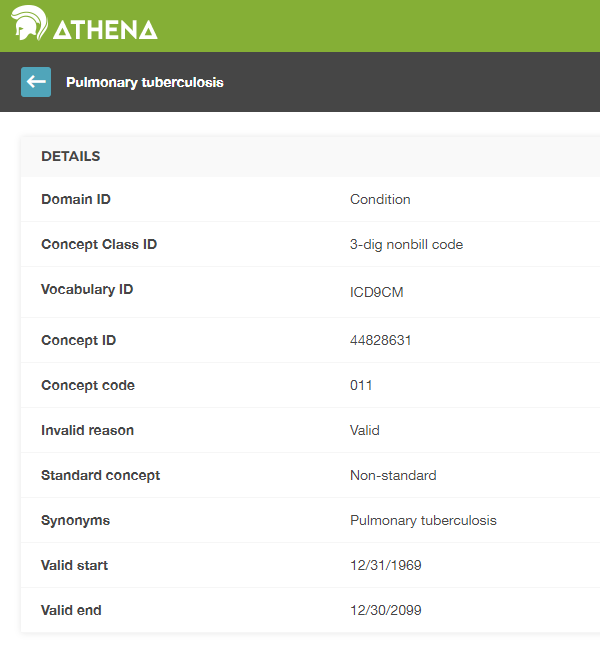
\includegraphics[width=0.75\linewidth]{images/CommonDataModel/pulmTubICD9} \caption{ICD9CM code for Pulmonary Tuberculosis}\label{fig:pulmTubICD9}
\end{figure}

Without the use of a standard way to represent TB the code 011 could be
interpreted as `Hospital Inpatient (Including Medicare Part A)' in the
UB04 vocabulary, or as `Nervous System Neoplasms without Complications,
Comorbidities' in the DRG vocabulary. This is where Concept IDs, both
Source and Standard, are valuable. The Concept ID that represents the
011 ICD9CM code is 44828631
\href{http://athena.ohdsi.org/search-terms/terms/44828631}{(http://athena.ohdsi.org/search-terms/terms/44828631)}.
This differentiates the ICD9CM from the UBO4 and from the DRG. The
Standard Concept that ICD9CM code maps to is 253954
\href{http://athena.ohdsi.org/search-terms/terms/253954}{(http://athena.ohdsi.org/search-terms/terms/253954)}
as shown in figure \ref{fig:pulmTubMap} by the relationship
`Non-standard to Standard map (OMOP)'. This same mapping relationship
exists between Read, ICD10, CIEL, and MeSH codes, among others, so that
any research that references the standard SNOMED concept is sure to
include all supported source codes.

\begin{figure}
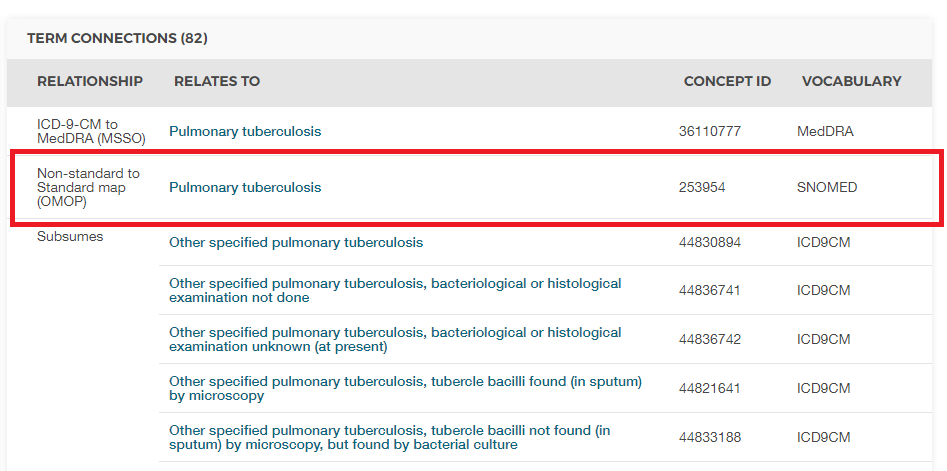
\includegraphics[width=1\linewidth]{images/CommonDataModel/pulmTubMap} \caption{SNOMED code for Pulmonary Tuberculosis}\label{fig:pulmTubMap}
\end{figure}

An example of how this relationship is depicted in the tables is shown
in figure (\textbf{link to figure in CONDITION\_OCCURRENCE})

\section{OMOP CDM Standardized
Tables}\label{omop-cdm-standardized-tables}

The OMOP CDM contains 16 Clinical data tables, 10 Vocabulary tables, 2
Metadata tables, 4 Health System data tables, 2 Health Economics data
tables, 3 standardized derived elements, and 2 results schema tables. To
illustrate how these tables are utilized in practice the data of one
person will be used as a common thread throughout the rest of the
chapter. While part of the CDM the Vocabulary tables are not covered
here, rather, they are detailed in depth in Chapter
\ref{StandardizedVocabularies}.

\subsection{Running Example:
Endometriosis}\label{running-example-endometriosis}

Endometriosis is a painful condition whereby cells normally found in the
lining of a woman's uterus occur elsewhere in the body. Severe cases can
lead to infertility, bowel, and bladder problems. The following sections
will detail one patient's experience with this disease and how her
clinical experience might be represented in the Common Data Model.

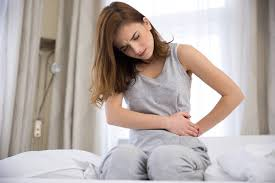
\includegraphics[width=0.5\linewidth]{images/CommonDataModel/Lauren}

\begin{figure}
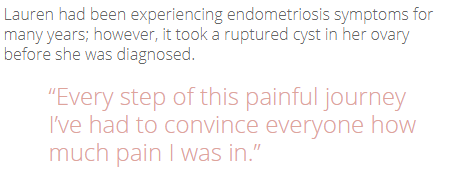
\includegraphics[width=0.75\linewidth]{images/CommonDataModel/laurentext} \caption{Read more about Lauren and endometriosis at https://www.endometriosis-uk.org/laurens-story}\label{fig:Laurentext}
\end{figure}

\subsection{PERSON table}\label{person}

As the Common Data Model is a person-centric model (see section
\ref{model-conv}) let's start with how she would be represented in the
PERSON table. For the full PERSON table specification please see the CDM
wiki \url{https://github.com/OHDSI/CommonDataModel/wiki/PERSON}.

\textbf{What do we know about Lauren?}

\begin{itemize}
\tightlist
\item
  She is a 36-year-old woman
\item
  Her birthday is 12-March-1982
\item
  She is white
\item
  She is english
\end{itemize}

With that in mind, her PERSON table might look something like this:

\begin{longtable}[]{@{}lll@{}}
\toprule
\begin{minipage}[b]{0.33\columnwidth}\raggedright\strut
Column Name\strut
\end{minipage} & \begin{minipage}[b]{0.16\columnwidth}\raggedright\strut
Value\strut
\end{minipage} & \begin{minipage}[b]{0.42\columnwidth}\raggedright\strut
Explanation\strut
\end{minipage}\tabularnewline
\midrule
\endhead
\begin{minipage}[t]{0.33\columnwidth}\raggedright\strut
person\_id\strut
\end{minipage} & \begin{minipage}[t]{0.16\columnwidth}\raggedright\strut
1\strut
\end{minipage} & \begin{minipage}[t]{0.42\columnwidth}\raggedright\strut
Person\_id should be an integer, either directly from the source or
generated as part of the build process.\strut
\end{minipage}\tabularnewline
\begin{minipage}[t]{0.33\columnwidth}\raggedright\strut
gender\_concept\_id\strut
\end{minipage} & \begin{minipage}[t]{0.16\columnwidth}\raggedright\strut
8532\strut
\end{minipage} & \begin{minipage}[t]{0.42\columnwidth}\raggedright\strut
The concept\_id referring to female gender is 8532
\href{http://athena.ohdsi.org/search-terms/terms/8532}{(http://athena.ohdsi.org/search-terms/terms/8532)}.\strut
\end{minipage}\tabularnewline
\begin{minipage}[t]{0.33\columnwidth}\raggedright\strut
year\_of\_birth\strut
\end{minipage} & \begin{minipage}[t]{0.16\columnwidth}\raggedright\strut
1982\strut
\end{minipage} & \begin{minipage}[t]{0.42\columnwidth}\raggedright\strut
\strut
\end{minipage}\tabularnewline
\begin{minipage}[t]{0.33\columnwidth}\raggedright\strut
month\_of\_birth\strut
\end{minipage} & \begin{minipage}[t]{0.16\columnwidth}\raggedright\strut
3\strut
\end{minipage} & \begin{minipage}[t]{0.42\columnwidth}\raggedright\strut
\strut
\end{minipage}\tabularnewline
\begin{minipage}[t]{0.33\columnwidth}\raggedright\strut
day\_of\_birth\strut
\end{minipage} & \begin{minipage}[t]{0.16\columnwidth}\raggedright\strut
12\strut
\end{minipage} & \begin{minipage}[t]{0.42\columnwidth}\raggedright\strut
\strut
\end{minipage}\tabularnewline
\begin{minipage}[t]{0.33\columnwidth}\raggedright\strut
birth\_datetime\strut
\end{minipage} & \begin{minipage}[t]{0.16\columnwidth}\raggedright\strut
1982-03-12 00:00:00\strut
\end{minipage} & \begin{minipage}[t]{0.42\columnwidth}\raggedright\strut
When the time is not known midnight is used.\strut
\end{minipage}\tabularnewline
\begin{minipage}[t]{0.33\columnwidth}\raggedright\strut
death\_datetime\strut
\end{minipage} & \begin{minipage}[t]{0.16\columnwidth}\raggedright\strut
\strut
\end{minipage} & \begin{minipage}[t]{0.42\columnwidth}\raggedright\strut
\strut
\end{minipage}\tabularnewline
\begin{minipage}[t]{0.33\columnwidth}\raggedright\strut
race\_concept\_id\strut
\end{minipage} & \begin{minipage}[t]{0.16\columnwidth}\raggedright\strut
8527\strut
\end{minipage} & \begin{minipage}[t]{0.42\columnwidth}\raggedright\strut
The concept\_id referring to white race is 8527
\href{http://athena.ohdsi.org/search-terms/terms/8527}{(http://athena.ohdsi.org/search-terms/terms/8527)}.\strut
\end{minipage}\tabularnewline
\begin{minipage}[t]{0.33\columnwidth}\raggedright\strut
ethnicity\_concept\_id\strut
\end{minipage} & \begin{minipage}[t]{0.16\columnwidth}\raggedright\strut
38003564\strut
\end{minipage} & \begin{minipage}[t]{0.42\columnwidth}\raggedright\strut
Typically hispanic status is stored for ethnicity. The concept\_id
38003564
\href{http://athena.ohdsi.org/search-terms/terms/38003564}{(http://athena.ohdsi.org/search-terms/terms/38003564)}
refers to `Not hispanic'.\strut
\end{minipage}\tabularnewline
\begin{minipage}[t]{0.33\columnwidth}\raggedright\strut
location\_id\strut
\end{minipage} & \begin{minipage}[t]{0.16\columnwidth}\raggedright\strut
\strut
\end{minipage} & \begin{minipage}[t]{0.42\columnwidth}\raggedright\strut
Her address is not known.\strut
\end{minipage}\tabularnewline
\begin{minipage}[t]{0.33\columnwidth}\raggedright\strut
provider\_id\strut
\end{minipage} & \begin{minipage}[t]{0.16\columnwidth}\raggedright\strut
\strut
\end{minipage} & \begin{minipage}[t]{0.42\columnwidth}\raggedright\strut
Her primary care provider is not known.\strut
\end{minipage}\tabularnewline
\begin{minipage}[t]{0.33\columnwidth}\raggedright\strut
care\_site\_id\strut
\end{minipage} & \begin{minipage}[t]{0.16\columnwidth}\raggedright\strut
\strut
\end{minipage} & \begin{minipage}[t]{0.42\columnwidth}\raggedright\strut
Her primary care site is not known.\strut
\end{minipage}\tabularnewline
\begin{minipage}[t]{0.33\columnwidth}\raggedright\strut
person\_source\_value\strut
\end{minipage} & \begin{minipage}[t]{0.16\columnwidth}\raggedright\strut
1\strut
\end{minipage} & \begin{minipage}[t]{0.42\columnwidth}\raggedright\strut
Typically this would be her identifier in the source data, though often
is it the same as the person\_id.\strut
\end{minipage}\tabularnewline
\begin{minipage}[t]{0.33\columnwidth}\raggedright\strut
gender\_source\_value\strut
\end{minipage} & \begin{minipage}[t]{0.16\columnwidth}\raggedright\strut
F\strut
\end{minipage} & \begin{minipage}[t]{0.42\columnwidth}\raggedright\strut
The gender value as it appears in the source is stored here.\strut
\end{minipage}\tabularnewline
\begin{minipage}[t]{0.33\columnwidth}\raggedright\strut
gender\_source\_concept\_id\strut
\end{minipage} & \begin{minipage}[t]{0.16\columnwidth}\raggedright\strut
0\strut
\end{minipage} & \begin{minipage}[t]{0.42\columnwidth}\raggedright\strut
If the gender value in the source was coded using a vocabulary
recognized by OHDSI, that concept\_id would go here. For example, if her
gender was `Sex-F' in the source and it was stated to be in the PCORNet
vocabulary concept\_id 44814665
\href{http://athena.ohdsi.org/search-terms/terms/44814665}{(http://athena.ohdsi.org/search-terms/terms/44814665)}
would go in this field.\strut
\end{minipage}\tabularnewline
\begin{minipage}[t]{0.33\columnwidth}\raggedright\strut
race\_source\_value\strut
\end{minipage} & \begin{minipage}[t]{0.16\columnwidth}\raggedright\strut
white\strut
\end{minipage} & \begin{minipage}[t]{0.42\columnwidth}\raggedright\strut
The race value as it appears in the source is stored here.\strut
\end{minipage}\tabularnewline
\begin{minipage}[t]{0.33\columnwidth}\raggedright\strut
race\_source\_concept\_id\strut
\end{minipage} & \begin{minipage}[t]{0.16\columnwidth}\raggedright\strut
0\strut
\end{minipage} & \begin{minipage}[t]{0.42\columnwidth}\raggedright\strut
Same principle as gender\_source\_concept\_id.\strut
\end{minipage}\tabularnewline
\begin{minipage}[t]{0.33\columnwidth}\raggedright\strut
ethnicity\_source\_value\strut
\end{minipage} & \begin{minipage}[t]{0.16\columnwidth}\raggedright\strut
english\strut
\end{minipage} & \begin{minipage}[t]{0.42\columnwidth}\raggedright\strut
The ethnicity value as it appears in the source is stored here.\strut
\end{minipage}\tabularnewline
\begin{minipage}[t]{0.33\columnwidth}\raggedright\strut
ethnicity\_source\_concept\_id\strut
\end{minipage} & \begin{minipage}[t]{0.16\columnwidth}\raggedright\strut
0\strut
\end{minipage} & \begin{minipage}[t]{0.42\columnwidth}\raggedright\strut
Same principle as gender\_source\_concept\_id.\strut
\end{minipage}\tabularnewline
\bottomrule
\end{longtable}

\subsection{OBSERVATION\_PERIOD table}\label{observationPeriod}

The OBSERVATION\_PERIOD table is designed to define the amount of time
for which a patient's clinical events are recorded in the source system.
For US healthcare insurance claims this is typically the enrollment
period of the patient. When working with data from electronic health
records (EHR) often the first record in the system is considered the
observation\_period\_start\_date and the latest record is considered the
observation\_period\_end\_date with the understanding that only the
clinical events that happened within that particular system were
recorded. For the full OBSERVATION\_PERIOD table specification please
see the CDM wiki
\href{https://github.com/OHDSI/CommonDataModel/wiki/OBSERVATION_PERIOD}{(https://github.com/OHDSI/CommonDataModel/wiki/OBSERVATION\_PERIOD)}.

\textbf{How can we determine Lauren's observation period?}

Lauren's information is most similar to EHR data in that we only have
records of her encounters from which to determine her observation
period.

\begin{longtable}[]{@{}llll@{}}
\toprule
Encounter\_ID & Start\_Date & Stop\_Date & EncounterClass\tabularnewline
\midrule
\endhead
70 & 2010-01-06 & 2010-01-06 & outpatient\tabularnewline
80 & 2011-01-06 & 2011-01-06 & outpatient\tabularnewline
90 & 2012-01-06 & 2012-01-06 & outpatient\tabularnewline
100 & 2013-01-07 & 2013-01-07 & outpatient\tabularnewline
101 & 2013-01-14 & 2013-01-14 & ambulatory\tabularnewline
102 & 2013-01-17 & 2013-01-24 & inpatient\tabularnewline
\bottomrule
\end{longtable}

Based on the encounter records her OBSERVATION\_PERIOD table might look
something like this:

\begin{longtable}[]{@{}lll@{}}
\toprule
\begin{minipage}[b]{0.33\columnwidth}\raggedright\strut
Column Name\strut
\end{minipage} & \begin{minipage}[b]{0.16\columnwidth}\raggedright\strut
Value\strut
\end{minipage} & \begin{minipage}[b]{0.42\columnwidth}\raggedright\strut
Explanation\strut
\end{minipage}\tabularnewline
\midrule
\endhead
\begin{minipage}[t]{0.33\columnwidth}\raggedright\strut
observation\_period\_id\strut
\end{minipage} & \begin{minipage}[t]{0.16\columnwidth}\raggedright\strut
1\strut
\end{minipage} & \begin{minipage}[t]{0.42\columnwidth}\raggedright\strut
This is typically an autogenerated field that creates a unique id number
for each record in the table.\strut
\end{minipage}\tabularnewline
\begin{minipage}[t]{0.33\columnwidth}\raggedright\strut
person\_id\strut
\end{minipage} & \begin{minipage}[t]{0.16\columnwidth}\raggedright\strut
1\strut
\end{minipage} & \begin{minipage}[t]{0.42\columnwidth}\raggedright\strut
This comes from the PERSON table and links PERSON and
OBSERVATION\_PERIOD.\strut
\end{minipage}\tabularnewline
\begin{minipage}[t]{0.33\columnwidth}\raggedright\strut
observation\_period\_start\_date\strut
\end{minipage} & \begin{minipage}[t]{0.16\columnwidth}\raggedright\strut
2010-01-06\strut
\end{minipage} & \begin{minipage}[t]{0.42\columnwidth}\raggedright\strut
This is the start date of her earliest encounter on record.\strut
\end{minipage}\tabularnewline
\begin{minipage}[t]{0.33\columnwidth}\raggedright\strut
observation\_period\_end\_date\strut
\end{minipage} & \begin{minipage}[t]{0.16\columnwidth}\raggedright\strut
2013-01-24\strut
\end{minipage} & \begin{minipage}[t]{0.42\columnwidth}\raggedright\strut
This is the end date of her latest encounter on record.\strut
\end{minipage}\tabularnewline
\begin{minipage}[t]{0.33\columnwidth}\raggedright\strut
period\_type\_concept\_id\strut
\end{minipage} & \begin{minipage}[t]{0.16\columnwidth}\raggedright\strut
44814725\strut
\end{minipage} & \begin{minipage}[t]{0.42\columnwidth}\raggedright\strut
The best option in the Vocabulary with the concept class `Obs Period
Type' is 44814724
\href{http://athena.ohdsi.org/search-terms/terms/44814724}{(http://athena.ohdsi.org/search-terms/terms/44814724)},
which stands for `Period covering healthcare encounters'.\strut
\end{minipage}\tabularnewline
\bottomrule
\end{longtable}

\subsection{VISIT\_OCCURRENCE}\label{visitOccurrence}

The VISIT\_OCCURRENCE table houses information about a patient's
encounters with the health care system. Within the OHDSI vernacular
these are referred to as visits and are considered to be discreet
events. There are 12 categories of visits though the most common are
inpatient, outpatient, emergency and long term care. For the full
VISIT\_OCCURRENCE table specification please see the CDM wiki
\href{https://github.com/OHDSI/CommonDataModel/wiki/VISIT_OCCURRENCE}{(https://github.com/OHDSI/CommonDataModel/wiki/VISIT\_OCCURRENCE)}.

\textbf{How do we represent Lauren's encounters as visits?}

Revisting the encounters we used to determine her observation period:

\begin{longtable}[]{@{}llll@{}}
\toprule
Encounter\_ID & Start\_Date & Stop\_Date & EncounterClass\tabularnewline
\midrule
\endhead
70 & 2010-01-06 & 2010-01-06 & outpatient\tabularnewline
80 & 2011-01-06 & 2011-01-06 & outpatient\tabularnewline
90 & 2012-01-06 & 2012-01-06 & outpatient\tabularnewline
100 & 2013-01-07 & 2013-01-07 & outpatient\tabularnewline
101 & 2013-01-14 & 2013-01-14 & ambulatory\tabularnewline
\textbf{102} & \textbf{2013-01-17} & \textbf{2013-01-24} &
\textbf{inpatient}\tabularnewline
\bottomrule
\end{longtable}

As an example let's represent the inpatient encounter as a record in the
VISIT\_OCCURRENCE table.

\begin{longtable}[]{@{}lll@{}}
\toprule
\begin{minipage}[b]{0.25\columnwidth}\raggedright\strut
Column Name\strut
\end{minipage} & \begin{minipage}[b]{0.17\columnwidth}\raggedright\strut
Value\strut
\end{minipage} & \begin{minipage}[b]{0.49\columnwidth}\raggedright\strut
Explanation\strut
\end{minipage}\tabularnewline
\midrule
\endhead
\begin{minipage}[t]{0.25\columnwidth}\raggedright\strut
visit\_occurrence\_id\strut
\end{minipage} & \begin{minipage}[t]{0.17\columnwidth}\raggedright\strut
514\strut
\end{minipage} & \begin{minipage}[t]{0.49\columnwidth}\raggedright\strut
This is typically an autogenerated field that creates a unique id number
for each visit on the person's record in the converted CDM
database.\strut
\end{minipage}\tabularnewline
\begin{minipage}[t]{0.25\columnwidth}\raggedright\strut
person\_id\strut
\end{minipage} & \begin{minipage}[t]{0.17\columnwidth}\raggedright\strut
1\strut
\end{minipage} & \begin{minipage}[t]{0.49\columnwidth}\raggedright\strut
This comes from the PERSON table and links PERSON and
VISIT\_OCCURRENCE.\strut
\end{minipage}\tabularnewline
\begin{minipage}[t]{0.25\columnwidth}\raggedright\strut
visit\_concept\_id\strut
\end{minipage} & \begin{minipage}[t]{0.17\columnwidth}\raggedright\strut
9201\strut
\end{minipage} & \begin{minipage}[t]{0.49\columnwidth}\raggedright\strut
The concept\_id referring to an inpatient visit is 9201
\href{http://athena.ohdsi.org/search-terms/terms/9201}{(http://athena.ohdsi.org/search-terms/terms/9201)}.\strut
\end{minipage}\tabularnewline
\begin{minipage}[t]{0.25\columnwidth}\raggedright\strut
visit\_start\_date\strut
\end{minipage} & \begin{minipage}[t]{0.17\columnwidth}\raggedright\strut
2013-01-17\strut
\end{minipage} & \begin{minipage}[t]{0.49\columnwidth}\raggedright\strut
The start date of the visit.\strut
\end{minipage}\tabularnewline
\begin{minipage}[t]{0.25\columnwidth}\raggedright\strut
visit\_start\_datetime\strut
\end{minipage} & \begin{minipage}[t]{0.17\columnwidth}\raggedright\strut
2013-01-17 00:00:00\strut
\end{minipage} & \begin{minipage}[t]{0.49\columnwidth}\raggedright\strut
The date and time of the visit started. When time is unknown midnight is
used.\strut
\end{minipage}\tabularnewline
\begin{minipage}[t]{0.25\columnwidth}\raggedright\strut
visit\_end\_date\strut
\end{minipage} & \begin{minipage}[t]{0.17\columnwidth}\raggedright\strut
2013-01-24\strut
\end{minipage} & \begin{minipage}[t]{0.49\columnwidth}\raggedright\strut
The end date of the visit. If this is a one-day visit the end date
should match the start date.\strut
\end{minipage}\tabularnewline
\begin{minipage}[t]{0.25\columnwidth}\raggedright\strut
visit\_end\_datetime\strut
\end{minipage} & \begin{minipage}[t]{0.17\columnwidth}\raggedright\strut
2013-01-24 00:00:00\strut
\end{minipage} & \begin{minipage}[t]{0.49\columnwidth}\raggedright\strut
The date and time of the visit end. If time is unknown midnight is
used.\strut
\end{minipage}\tabularnewline
\begin{minipage}[t]{0.25\columnwidth}\raggedright\strut
visit\_type\_concept\_id\strut
\end{minipage} & \begin{minipage}[t]{0.17\columnwidth}\raggedright\strut
32034\strut
\end{minipage} & \begin{minipage}[t]{0.49\columnwidth}\raggedright\strut
This column is intended to provide information about the provenance of
the visit record, i.e.~does it come from an insurance claim, hospital
billing record, EHR record, etc. For this example the concept\_id 32035
\href{http://athena.ohdsi.org/search-terms/terms/32035}{(http://athena.ohdsi.org/search-terms/terms/32035)}
is used as the encounters are similar to electronic health records\strut
\end{minipage}\tabularnewline
\begin{minipage}[t]{0.25\columnwidth}\raggedright\strut
provider\_id*\strut
\end{minipage} & \begin{minipage}[t]{0.17\columnwidth}\raggedright\strut
NULL\strut
\end{minipage} & \begin{minipage}[t]{0.49\columnwidth}\raggedright\strut
If the encounter record has a provider associated, the id for that
provider goes in this field. This should be the provider\_id from the
PROVIDER table that represents the provider on the encounter.\strut
\end{minipage}\tabularnewline
\begin{minipage}[t]{0.25\columnwidth}\raggedright\strut
care\_site\_id\strut
\end{minipage} & \begin{minipage}[t]{0.17\columnwidth}\raggedright\strut
NULL\strut
\end{minipage} & \begin{minipage}[t]{0.49\columnwidth}\raggedright\strut
If the encounter record has a care site associated, the id for that care
site goes in this field. This should be the care\_site\_id from the
CARE\_SITE table that codes for the care site on the encounter.\strut
\end{minipage}\tabularnewline
\begin{minipage}[t]{0.25\columnwidth}\raggedright\strut
visit\_source\_value\strut
\end{minipage} & \begin{minipage}[t]{0.17\columnwidth}\raggedright\strut
inpatient\strut
\end{minipage} & \begin{minipage}[t]{0.49\columnwidth}\raggedright\strut
The visit value as it appears in the source goes here. In this context
`visit' means outpatient, inpatient, emergency, etc.\strut
\end{minipage}\tabularnewline
\begin{minipage}[t]{0.25\columnwidth}\raggedright\strut
visit\_source\_concept\_id\strut
\end{minipage} & \begin{minipage}[t]{0.17\columnwidth}\raggedright\strut
0\strut
\end{minipage} & \begin{minipage}[t]{0.49\columnwidth}\raggedright\strut
If the visit value from the source is coded using a vocabulary that is
recognized by OHDSI, the concept\_id that represents the visit source
value would go here.\strut
\end{minipage}\tabularnewline
\begin{minipage}[t]{0.25\columnwidth}\raggedright\strut
admitted\_from\_concept\_id\strut
\end{minipage} & \begin{minipage}[t]{0.17\columnwidth}\raggedright\strut
0\strut
\end{minipage} & \begin{minipage}[t]{0.49\columnwidth}\raggedright\strut
If known, this is the concept\_id that represents where the patient was
admitted from. This concept should have the concept class `Place of
Service' and the domain `Visit'. For example, if a patient was admitted
to the hospital from home, the concept\_id would be 8536
\href{http://athena.ohdsi.org/search-terms/terms/8536}{(http://athena.ohdsi.org/search-terms/terms/8536)}.\strut
\end{minipage}\tabularnewline
\begin{minipage}[t]{0.25\columnwidth}\raggedright\strut
admitted\_from\_source\_value\strut
\end{minipage} & \begin{minipage}[t]{0.17\columnwidth}\raggedright\strut
NULL\strut
\end{minipage} & \begin{minipage}[t]{0.49\columnwidth}\raggedright\strut
This is the value from the source that represents where the patient was
admitted from. Using the above example, this would be `home'.\strut
\end{minipage}\tabularnewline
\begin{minipage}[t]{0.25\columnwidth}\raggedright\strut
discharge\_to\_concept\_id\strut
\end{minipage} & \begin{minipage}[t]{0.17\columnwidth}\raggedright\strut
0\strut
\end{minipage} & \begin{minipage}[t]{0.49\columnwidth}\raggedright\strut
If known, this is the concept\_id that represents where the patient was
discharged to. This concept should have the concept class `Place of
Service' and the domain `Visit'. For example, if a patient was released
to an assisted living facility, the concept\_id would be 8615
\href{http://athena.ohdsi.org/search-terms/terms/8615}{(http://athena.ohdsi.org/search-terms/terms/8615)}.\strut
\end{minipage}\tabularnewline
\begin{minipage}[t]{0.25\columnwidth}\raggedright\strut
discharge\_to\_source\_value\strut
\end{minipage} & \begin{minipage}[t]{0.17\columnwidth}\raggedright\strut
0\strut
\end{minipage} & \begin{minipage}[t]{0.49\columnwidth}\raggedright\strut
This is the value from the source that represents where the patient was
discharged to. Using the above example, this would be `assisted living
facility'.\strut
\end{minipage}\tabularnewline
\begin{minipage}[t]{0.25\columnwidth}\raggedright\strut
preceding\_visit\_occurrence\_id\strut
\end{minipage} & \begin{minipage}[t]{0.17\columnwidth}\raggedright\strut
NULL\strut
\end{minipage} & \begin{minipage}[t]{0.49\columnwidth}\raggedright\strut
The visit\_occurrence\_id for the visit immediately preceding the
current one in time for the patient.\strut
\end{minipage}\tabularnewline
\bottomrule
\end{longtable}

*A patient may interact with multiple health care providers during one
visit, as is often the case with inpatient stays. These interactions can
be recorded in the VISIT\_DETAIL table. While not covered in depth in
this chapter, you can read more about the VISIT\_DETAIL table on the CDM
wiki
\href{https://github.com/OHDSI/CommonDataModel/wiki/VISIT_DETAIL}{(https://github.com/OHDSI/CommonDataModel/wiki/VISIT\_DETAIL)}

\subsection{CONDITION\_OCCURRENCE}\label{conditionOccurrence}

Records in the CONDITION\_OCCURRENCE table are diagnoses, signs, or
symptoms of a condition either observed by a Provider or reported by the
patient.

\textbf{What are Lauren's conditions?}

Revisiting her account she says ``About 3 years ago I noticed my
periods, which had also been painful, were getting increasingly more
painful. I started becoming aware of a sharp jabbing pain right by my
colon and feeling tender and bloated around my tailbone and lower pelvis
area. My periods had become so painful that I was missing 1-2 days of
work a month. Painkillers sometimes dulled the pain, but usually they
didn't do much.''

The SNOMED code for painful menstruation cramps, otherwise known as
dysmenorrhea, is 266599000. Let's see how that would be represented in
the CONDITION\_OCCURRENCE table:

\begin{longtable}[]{@{}lll@{}}
\toprule
\begin{minipage}[b]{0.27\columnwidth}\raggedright\strut
Column\strut
\end{minipage} & \begin{minipage}[b]{0.14\columnwidth}\raggedright\strut
Value\strut
\end{minipage} & \begin{minipage}[b]{0.50\columnwidth}\raggedright\strut
Explanation\strut
\end{minipage}\tabularnewline
\midrule
\endhead
\begin{minipage}[t]{0.27\columnwidth}\raggedright\strut
condition\_occurrence\_id\strut
\end{minipage} & \begin{minipage}[t]{0.14\columnwidth}\raggedright\strut
964\strut
\end{minipage} & \begin{minipage}[t]{0.50\columnwidth}\raggedright\strut
This is typically an autogenerated field that creates a unique id number
for each condition on the person's record in the converted CDM
database.\strut
\end{minipage}\tabularnewline
\begin{minipage}[t]{0.27\columnwidth}\raggedright\strut
person\_id\strut
\end{minipage} & \begin{minipage}[t]{0.14\columnwidth}\raggedright\strut
1\strut
\end{minipage} & \begin{minipage}[t]{0.50\columnwidth}\raggedright\strut
This comes from the PERSON table and links PERSON and
CONDITION\_OCCURRENCE.\strut
\end{minipage}\tabularnewline
\begin{minipage}[t]{0.27\columnwidth}\raggedright\strut
condition\_concept\_id\strut
\end{minipage} & \begin{minipage}[t]{0.14\columnwidth}\raggedright\strut
194696\strut
\end{minipage} & \begin{minipage}[t]{0.50\columnwidth}\raggedright\strut
The concept\_id that represents the SNOMED code 266599000 is 194696
\href{http://athena.ohdsi.org/search-terms/terms/194696}{(http://athena.ohdsi.org/search-terms/terms/194696)}\strut
\end{minipage}\tabularnewline
\begin{minipage}[t]{0.27\columnwidth}\raggedright\strut
condition\_start\_date\strut
\end{minipage} & \begin{minipage}[t]{0.14\columnwidth}\raggedright\strut
2010-01-06\strut
\end{minipage} & \begin{minipage}[t]{0.50\columnwidth}\raggedright\strut
The date when the instance of the Condition is recorded.\strut
\end{minipage}\tabularnewline
\begin{minipage}[t]{0.27\columnwidth}\raggedright\strut
condition\_start\_datetime\strut
\end{minipage} & \begin{minipage}[t]{0.14\columnwidth}\raggedright\strut
2010-01-06 00:00:00\strut
\end{minipage} & \begin{minipage}[t]{0.50\columnwidth}\raggedright\strut
The date and time when the instance of the Condition is recorded.
Midnight is used when the time is unknown\strut
\end{minipage}\tabularnewline
\begin{minipage}[t]{0.27\columnwidth}\raggedright\strut
condition\_end\_date\strut
\end{minipage} & \begin{minipage}[t]{0.14\columnwidth}\raggedright\strut
NULL\strut
\end{minipage} & \begin{minipage}[t]{0.50\columnwidth}\raggedright\strut
If known, this is the date when the instance of the Condition is
considered to have ended.\strut
\end{minipage}\tabularnewline
\begin{minipage}[t]{0.27\columnwidth}\raggedright\strut
condition\_end\_datetime\strut
\end{minipage} & \begin{minipage}[t]{0.14\columnwidth}\raggedright\strut
NULL\strut
\end{minipage} & \begin{minipage}[t]{0.50\columnwidth}\raggedright\strut
If known, this is the date and time when the instance of the Condition
is considered to have ended.\strut
\end{minipage}\tabularnewline
\begin{minipage}[t]{0.27\columnwidth}\raggedright\strut
condition\_type\_concept\_id\strut
\end{minipage} & \begin{minipage}[t]{0.14\columnwidth}\raggedright\strut
32020\strut
\end{minipage} & \begin{minipage}[t]{0.50\columnwidth}\raggedright\strut
This column is intended to provide information about the provenance of
the condition, i.e.~does it come from an insurance claim, hospital
billing record, EHR record, etc. For this example the concept\_id 32020
\href{http://athena.ohdsi.org/search-terms/terms/32020}{(http://athena.ohdsi.org/search-terms/terms/32020)}
is used as the encounters are similar to electronic health records.
Concept\_ids in this field should be in the `Condition Type'
vocabulary.\strut
\end{minipage}\tabularnewline
\begin{minipage}[t]{0.27\columnwidth}\raggedright\strut
condition\_status\_concept\_id\strut
\end{minipage} & \begin{minipage}[t]{0.14\columnwidth}\raggedright\strut
0\strut
\end{minipage} & \begin{minipage}[t]{0.50\columnwidth}\raggedright\strut
If known, the condition\_status\_concept\_id represents when and/or how
the condition was diagnosed. For example, a condition could be an
admitting diagnosis, in which case the concept\_id 4203942
\href{http://athena.ohdsi.org/search-terms/terms/4203942}{(http://athena.ohdsi.org/search-terms/terms/4203942)}
would be used.\strut
\end{minipage}\tabularnewline
\begin{minipage}[t]{0.27\columnwidth}\raggedright\strut
stop\_reason\strut
\end{minipage} & \begin{minipage}[t]{0.14\columnwidth}\raggedright\strut
NULL\strut
\end{minipage} & \begin{minipage}[t]{0.50\columnwidth}\raggedright\strut
If known, the reason that the Condition was no longer present, as
indicated in the source data.\strut
\end{minipage}\tabularnewline
\begin{minipage}[t]{0.27\columnwidth}\raggedright\strut
provider\_id\strut
\end{minipage} & \begin{minipage}[t]{0.14\columnwidth}\raggedright\strut
NULL\strut
\end{minipage} & \begin{minipage}[t]{0.50\columnwidth}\raggedright\strut
If the condition record has a diagnosing provider listed, the id for
that provider goes in this field. This should be the provider\_id from
the PROVIDER table that represents the provider on the encounter.\strut
\end{minipage}\tabularnewline
\begin{minipage}[t]{0.27\columnwidth}\raggedright\strut
visit\_occurrence\_id\strut
\end{minipage} & \begin{minipage}[t]{0.14\columnwidth}\raggedright\strut
509\strut
\end{minipage} & \begin{minipage}[t]{0.50\columnwidth}\raggedright\strut
If known, this is the visit (represented as visit\_occurrence\_id taken
from the VISIT\_OCCURRENCE table) during which the condition was
diagnosed.\strut
\end{minipage}\tabularnewline
\begin{minipage}[t]{0.27\columnwidth}\raggedright\strut
visit\_detail\_id\strut
\end{minipage} & \begin{minipage}[t]{0.14\columnwidth}\raggedright\strut
NULL\strut
\end{minipage} & \begin{minipage}[t]{0.50\columnwidth}\raggedright\strut
If known, this is the visit detail encounter (represented as
visit\_detail\_id from the VISIT\_DETAIL table) during which the
condition was diagnosed.\strut
\end{minipage}\tabularnewline
\begin{minipage}[t]{0.27\columnwidth}\raggedright\strut
condition\_source\_value\strut
\end{minipage} & \begin{minipage}[t]{0.14\columnwidth}\raggedright\strut
266599000\strut
\end{minipage} & \begin{minipage}[t]{0.50\columnwidth}\raggedright\strut
This is the value from the source that represents the condition. In
Lauren's case of dysmenorrhea the SNOMED code for that condition is
stored here and the standard concept\_id mapped from that code is stored
in CONDITION\_CONCEPT\_ID.\strut
\end{minipage}\tabularnewline
\begin{minipage}[t]{0.27\columnwidth}\raggedright\strut
condition\_source\_concept\_id\strut
\end{minipage} & \begin{minipage}[t]{0.14\columnwidth}\raggedright\strut
194696\strut
\end{minipage} & \begin{minipage}[t]{0.50\columnwidth}\raggedright\strut
If the condition value from the source is coded using a vocabulary that
is recognized by OHDSI, the concept\_id that represents that value would
go here. In the example of dysmennorhea the source value is a SNOMED
code so the concept\_id that represents that code is 194696. In this
case it is the same as the condition\_concept\_id since the SNOMED
vocabulary is the standard condition vocabulary\strut
\end{minipage}\tabularnewline
\begin{minipage}[t]{0.27\columnwidth}\raggedright\strut
condition\_status\_source\_value\strut
\end{minipage} & \begin{minipage}[t]{0.14\columnwidth}\raggedright\strut
0\strut
\end{minipage} & \begin{minipage}[t]{0.50\columnwidth}\raggedright\strut
If the condition status value from the source is coded using a
vocabulary that is recognized by OHDSI, the concept\_id that represents
that source value would go here.\strut
\end{minipage}\tabularnewline
\bottomrule
\end{longtable}

\subsection{DRUG\_EXPOSURE}\label{drugExposure}

The DRUG\_EXPOSURE captures records about the utilization of a Drug when
ingested or otherwise introduced into the body. Drugs include
prescription and over-the-counter medicines, vaccines, and
large-molecule biologic therapies. Radiological devices ingested or
applied locally do not count as Drugs.

Drug Exposure is inferred from clinical events associated with orders,
prescriptions written, pharmacy dispensings, procedural administrations,
and other patient-reported information.

\textbf{What are Lauren's drug exposures?}

We know that Lauren was given 60 acetaminophen 325mg oral tablets for 30
days (NDC code 69842087651) at her visit on 2010-01-06 to help with her
dysmenorrhea pain. Here's how that might look in the DRUG\_EXPOSURE
table:

\begin{longtable}[]{@{}lll@{}}
\toprule
\begin{minipage}[b]{0.30\columnwidth}\raggedright\strut
Column\strut
\end{minipage} & \begin{minipage}[b]{0.14\columnwidth}\raggedright\strut
Value\strut
\end{minipage} & \begin{minipage}[b]{0.47\columnwidth}\raggedright\strut
Explanation\strut
\end{minipage}\tabularnewline
\midrule
\endhead
\begin{minipage}[t]{0.30\columnwidth}\raggedright\strut
drug\_exposure\_id\strut
\end{minipage} & \begin{minipage}[t]{0.14\columnwidth}\raggedright\strut
1001\strut
\end{minipage} & \begin{minipage}[t]{0.47\columnwidth}\raggedright\strut
This is typically an autogenerated field that creates a unique id number
for each drug\_exposure on the person's record in the converted CDM
database.\strut
\end{minipage}\tabularnewline
\begin{minipage}[t]{0.30\columnwidth}\raggedright\strut
person\_id\strut
\end{minipage} & \begin{minipage}[t]{0.14\columnwidth}\raggedright\strut
1\strut
\end{minipage} & \begin{minipage}[t]{0.47\columnwidth}\raggedright\strut
This comes from the PERSON table and links PERSON and
DRUG\_EXPOSURE.\strut
\end{minipage}\tabularnewline
\begin{minipage}[t]{0.30\columnwidth}\raggedright\strut
drug\_concept\_id\strut
\end{minipage} & \begin{minipage}[t]{0.14\columnwidth}\raggedright\strut
1127433\strut
\end{minipage} & \begin{minipage}[t]{0.47\columnwidth}\raggedright\strut
The NDC code for acetaminophen maps to the RxNorm code 313782 which is
represented by the concept\_id 1127433
\href{http://athena.ohdsi.org/search-terms/terms/1127433}{(http://athena.ohdsi.org/search-terms/terms/1127433)}.\strut
\end{minipage}\tabularnewline
\begin{minipage}[t]{0.30\columnwidth}\raggedright\strut
drug\_exposure\_start\_date\strut
\end{minipage} & \begin{minipage}[t]{0.14\columnwidth}\raggedright\strut
2010-01-06\strut
\end{minipage} & \begin{minipage}[t]{0.47\columnwidth}\raggedright\strut
The start date of the drug exposure\strut
\end{minipage}\tabularnewline
\begin{minipage}[t]{0.30\columnwidth}\raggedright\strut
drug\_exposure\_start\_datetime\strut
\end{minipage} & \begin{minipage}[t]{0.14\columnwidth}\raggedright\strut
2010-01-06 00:00:00\strut
\end{minipage} & \begin{minipage}[t]{0.47\columnwidth}\raggedright\strut
The start date and time of the drug exposure. Midnight is used when the
time is not known.\strut
\end{minipage}\tabularnewline
\begin{minipage}[t]{0.30\columnwidth}\raggedright\strut
drug\_exposure\_end\_date\strut
\end{minipage} & \begin{minipage}[t]{0.14\columnwidth}\raggedright\strut
2010-02-05\strut
\end{minipage} & \begin{minipage}[t]{0.47\columnwidth}\raggedright\strut
The end date of the drug exposure. Depending on different sources, it
could be a known or an inferred date and denotes the last day at which
the patient was still exposed to the drug. In this case the end is
inferred since we know Lauren had a 30 days supply.\strut
\end{minipage}\tabularnewline
\begin{minipage}[t]{0.30\columnwidth}\raggedright\strut
drug\_exposure\_end\_datetime\strut
\end{minipage} & \begin{minipage}[t]{0.14\columnwidth}\raggedright\strut
2010-02-05 00:00:00\strut
\end{minipage} & \begin{minipage}[t]{0.47\columnwidth}\raggedright\strut
The end date and time of the drug exposure. Similar rules apply as to
drug\_exposure\_end\_date. Midnight is used when time is unknown\strut
\end{minipage}\tabularnewline
\begin{minipage}[t]{0.30\columnwidth}\raggedright\strut
verbatim\_end\_date\strut
\end{minipage} & \begin{minipage}[t]{0.14\columnwidth}\raggedright\strut
NULL\strut
\end{minipage} & \begin{minipage}[t]{0.47\columnwidth}\raggedright\strut
If the source provides an end date rather than just days supply that
date goes here.\strut
\end{minipage}\tabularnewline
\begin{minipage}[t]{0.30\columnwidth}\raggedright\strut
drug\_type\_concept\_id\strut
\end{minipage} & \begin{minipage}[t]{0.14\columnwidth}\raggedright\strut
38000177\strut
\end{minipage} & \begin{minipage}[t]{0.47\columnwidth}\raggedright\strut
This column is intended to provide information about the provenance of
the drug, i.e.~does it come from an insurance claim, prescription
record, etc. For this example the concept\_id 38000177
\href{http://athena.ohdsi.org/search-terms/terms/38000177}{(http://athena.ohdsi.org/search-terms/terms/38000177)}
is used as the drug record is from a written prescription. Concept\_ids
in this field should be in the `Drug Type' vocabulary.\strut
\end{minipage}\tabularnewline
\begin{minipage}[t]{0.30\columnwidth}\raggedright\strut
stop\_reason\strut
\end{minipage} & \begin{minipage}[t]{0.14\columnwidth}\raggedright\strut
NULL\strut
\end{minipage} & \begin{minipage}[t]{0.47\columnwidth}\raggedright\strut
The reason the Drug was stopped. Reasons include regimen completed,
changed, removed, etc.\strut
\end{minipage}\tabularnewline
\begin{minipage}[t]{0.30\columnwidth}\raggedright\strut
refills\strut
\end{minipage} & \begin{minipage}[t]{0.14\columnwidth}\raggedright\strut
NULL\strut
\end{minipage} & \begin{minipage}[t]{0.47\columnwidth}\raggedright\strut
The number of refills after the initial prescription. The initial
prescription is not counted, values start with null. In the case of
Lauren's acetaminophen she did not have any refills so the value is
NULL.\strut
\end{minipage}\tabularnewline
\begin{minipage}[t]{0.30\columnwidth}\raggedright\strut
quantity\strut
\end{minipage} & \begin{minipage}[t]{0.14\columnwidth}\raggedright\strut
60\strut
\end{minipage} & \begin{minipage}[t]{0.47\columnwidth}\raggedright\strut
The quantity of drug as recorded in the original prescription or
dispensing record.\strut
\end{minipage}\tabularnewline
\begin{minipage}[t]{0.30\columnwidth}\raggedright\strut
days\_supply\strut
\end{minipage} & \begin{minipage}[t]{0.14\columnwidth}\raggedright\strut
30\strut
\end{minipage} & \begin{minipage}[t]{0.47\columnwidth}\raggedright\strut
The number of days of supply of the medication as prescribed.\strut
\end{minipage}\tabularnewline
\begin{minipage}[t]{0.30\columnwidth}\raggedright\strut
sig\strut
\end{minipage} & \begin{minipage}[t]{0.14\columnwidth}\raggedright\strut
NULL\strut
\end{minipage} & \begin{minipage}[t]{0.47\columnwidth}\raggedright\strut
The directions (`signetur') on the Drug prescription as recorded in the
original prescription (and printed on the container) or dispensing
record.\strut
\end{minipage}\tabularnewline
\begin{minipage}[t]{0.30\columnwidth}\raggedright\strut
route\_concept\_id\strut
\end{minipage} & \begin{minipage}[t]{0.14\columnwidth}\raggedright\strut
4132161\strut
\end{minipage} & \begin{minipage}[t]{0.47\columnwidth}\raggedright\strut
This concept is meant to represent the route of the drug the patient was
was exposed to. Lauren took her acetaminophen orally so the concept\_id
4132161
\href{http://athena.ohdsi.org/search-terms/terms/4132161}{(http://athena.ohdsi.org/search-terms/terms/4132161)}
is used.\strut
\end{minipage}\tabularnewline
\begin{minipage}[t]{0.30\columnwidth}\raggedright\strut
lot\_number\strut
\end{minipage} & \begin{minipage}[t]{0.14\columnwidth}\raggedright\strut
NULL\strut
\end{minipage} & \begin{minipage}[t]{0.47\columnwidth}\raggedright\strut
An identifier assigned to a particular quantity or lot of Drug product
from the manufacturer.\strut
\end{minipage}\tabularnewline
\begin{minipage}[t]{0.30\columnwidth}\raggedright\strut
provider\_id\strut
\end{minipage} & \begin{minipage}[t]{0.14\columnwidth}\raggedright\strut
NULL\strut
\end{minipage} & \begin{minipage}[t]{0.47\columnwidth}\raggedright\strut
If the drug record has a prescribing provider listed, the id for that
provider goes in this field. This should be the provider\_id from the
PROVIDER table that represents the provider on the encounter.\strut
\end{minipage}\tabularnewline
\begin{minipage}[t]{0.30\columnwidth}\raggedright\strut
visit\_occurrence\_id\strut
\end{minipage} & \begin{minipage}[t]{0.14\columnwidth}\raggedright\strut
509\strut
\end{minipage} & \begin{minipage}[t]{0.47\columnwidth}\raggedright\strut
If known, this is the visit (represented as visit\_occurrence\_id taken
from the VISIT\_OCCURRENCE table) during which the drug was
prescribed.\strut
\end{minipage}\tabularnewline
\begin{minipage}[t]{0.30\columnwidth}\raggedright\strut
visit\_detail\_id\strut
\end{minipage} & \begin{minipage}[t]{0.14\columnwidth}\raggedright\strut
NULL\strut
\end{minipage} & \begin{minipage}[t]{0.47\columnwidth}\raggedright\strut
If known, this is the visit detail (represented as visit\_detail\_id
taken from the VISIT\_DETAIL table) during which the drug was
prescribed.\strut
\end{minipage}\tabularnewline
\begin{minipage}[t]{0.30\columnwidth}\raggedright\strut
drug\_source\_value\strut
\end{minipage} & \begin{minipage}[t]{0.14\columnwidth}\raggedright\strut
69842087651\strut
\end{minipage} & \begin{minipage}[t]{0.47\columnwidth}\raggedright\strut
This is the source code for the Drug as it appears in the source data.
In Lauren's case she was prescribed acetaminophen and the NDC code is
stored here.\strut
\end{minipage}\tabularnewline
\begin{minipage}[t]{0.30\columnwidth}\raggedright\strut
drug\_source\_concept\_id\strut
\end{minipage} & \begin{minipage}[t]{0.14\columnwidth}\raggedright\strut
750264\strut
\end{minipage} & \begin{minipage}[t]{0.47\columnwidth}\raggedright\strut
This is the concept\_id that represents the drug source value. In this
example the concept\_id is 750264
\href{http://athena.ohdsi.org/search-terms/terms/750264}{(http://athena.ohdsi.org/search-terms/terms/750264)}.\strut
\end{minipage}\tabularnewline
\begin{minipage}[t]{0.30\columnwidth}\raggedright\strut
route\_source\_value\strut
\end{minipage} & \begin{minipage}[t]{0.14\columnwidth}\raggedright\strut
NULL\strut
\end{minipage} & \begin{minipage}[t]{0.47\columnwidth}\raggedright\strut
The information about the route of administration as detailed in the
source.\strut
\end{minipage}\tabularnewline
\begin{minipage}[t]{0.30\columnwidth}\raggedright\strut
dose\_unit\_source\_value\strut
\end{minipage} & \begin{minipage}[t]{0.14\columnwidth}\raggedright\strut
NULL\strut
\end{minipage} & \begin{minipage}[t]{0.47\columnwidth}\raggedright\strut
The information about the dose unit as detailed in the source.\strut
\end{minipage}\tabularnewline
\bottomrule
\end{longtable}

\subsection{PROCEDURE\_OCCURRENCE}\label{procedureOccurrence}

The PROCEDURE\_OCCURRENCE table contains records of activities or
processes ordered by, or carried out by, a healthcare provider on the
patient to have a diagnostic or therapeutic purpose. Procedures are
present in various data sources in different forms with varying levels
of standardization. For example:

\begin{itemize}
\tightlist
\item
  Medical Claims include procedure codes that are submitted as part of a
  claim for health services rendered, including procedures performed.
\item
  Electronic Health Records that capture procedures as orders.
\end{itemize}

\textbf{What procedures did Lauren have?} From her description we know
she had a ultrasound of her left ovary on 2013-01-14 that showed a 4x5cm
cyst. Here's how that would look in the PROCEDURE\_OCCURRENCE table:

\begin{longtable}[]{@{}lll@{}}
\toprule
\begin{minipage}[b]{0.30\columnwidth}\raggedright\strut
Column\strut
\end{minipage} & \begin{minipage}[b]{0.14\columnwidth}\raggedright\strut
Value\strut
\end{minipage} & \begin{minipage}[b]{0.47\columnwidth}\raggedright\strut
Explanation\strut
\end{minipage}\tabularnewline
\midrule
\endhead
\begin{minipage}[t]{0.30\columnwidth}\raggedright\strut
procedure\_occurrence\_id\strut
\end{minipage} & \begin{minipage}[t]{0.14\columnwidth}\raggedright\strut
1277\strut
\end{minipage} & \begin{minipage}[t]{0.47\columnwidth}\raggedright\strut
This is typically an autogenerated field that creates a unique id number
for each procedure\_occurrence on the person's record in the converted
CDM database.\strut
\end{minipage}\tabularnewline
\begin{minipage}[t]{0.30\columnwidth}\raggedright\strut
person\_id\strut
\end{minipage} & \begin{minipage}[t]{0.14\columnwidth}\raggedright\strut
1\strut
\end{minipage} & \begin{minipage}[t]{0.47\columnwidth}\raggedright\strut
This comes from the PERSON table and links PERSON and
PROCEDURE\_OCCURRENCE\strut
\end{minipage}\tabularnewline
\begin{minipage}[t]{0.30\columnwidth}\raggedright\strut
procedure\_concept\_id\strut
\end{minipage} & \begin{minipage}[t]{0.14\columnwidth}\raggedright\strut
4127451\strut
\end{minipage} & \begin{minipage}[t]{0.47\columnwidth}\raggedright\strut
The SNOMED procedure code for a pelvic ultrasound is 304435002 which is
represented by the concept\_id 4127451
\href{http://athena.ohdsi.org/search-terms/terms/4127451}{(http://athena.ohdsi.org/search-terms/terms/4127451)}.\strut
\end{minipage}\tabularnewline
\begin{minipage}[t]{0.30\columnwidth}\raggedright\strut
procedure\_date\strut
\end{minipage} & \begin{minipage}[t]{0.14\columnwidth}\raggedright\strut
2013-01-14\strut
\end{minipage} & \begin{minipage}[t]{0.47\columnwidth}\raggedright\strut
The date on which the procedure was performed.\strut
\end{minipage}\tabularnewline
\begin{minipage}[t]{0.30\columnwidth}\raggedright\strut
procedure\_datetime\strut
\end{minipage} & \begin{minipage}[t]{0.14\columnwidth}\raggedright\strut
2013-01-14 00:00:00\strut
\end{minipage} & \begin{minipage}[t]{0.47\columnwidth}\raggedright\strut
The date and time on which the procedure was performed. Midnight is used
when time is unknown.\strut
\end{minipage}\tabularnewline
\begin{minipage}[t]{0.30\columnwidth}\raggedright\strut
procedure\_type\_concept\_id\strut
\end{minipage} & \begin{minipage}[t]{0.14\columnwidth}\raggedright\strut
38000275\strut
\end{minipage} & \begin{minipage}[t]{0.47\columnwidth}\raggedright\strut
This column is intended to provide information about the provenance of
the procedure, i.e.~does it come from an insurance claim, EHR order,
etc. For this example the concept\_id 38000275
\href{http://athena.ohdsi.org/search-terms/terms/38000275}{(http://athena.ohdsi.org/search-terms/terms/38000275)}
is used as the procedure record is from an EHR record. Concept\_ids in
this field should be in the `Procedure Type' vocabulary.\strut
\end{minipage}\tabularnewline
\begin{minipage}[t]{0.30\columnwidth}\raggedright\strut
modifier\_concept\_id\strut
\end{minipage} & \begin{minipage}[t]{0.14\columnwidth}\raggedright\strut
0\strut
\end{minipage} & \begin{minipage}[t]{0.47\columnwidth}\raggedright\strut
This is meant for a concept\_id representing the modifier on the
procedure. For example, if the record indicated that a CPT4 procedure
was performed bilaterally then the concept\_id 42739579
\href{http://athena.ohdsi.org/search-terms/terms/42739579}{(http://athena.ohdsi.org/search-terms/terms/42739579)}
would be used.\strut
\end{minipage}\tabularnewline
\begin{minipage}[t]{0.30\columnwidth}\raggedright\strut
quantity\strut
\end{minipage} & \begin{minipage}[t]{0.14\columnwidth}\raggedright\strut
0\strut
\end{minipage} & \begin{minipage}[t]{0.47\columnwidth}\raggedright\strut
The quantity of procedures ordered or administered.\strut
\end{minipage}\tabularnewline
\begin{minipage}[t]{0.30\columnwidth}\raggedright\strut
provider\_id\strut
\end{minipage} & \begin{minipage}[t]{0.14\columnwidth}\raggedright\strut
NULL\strut
\end{minipage} & \begin{minipage}[t]{0.47\columnwidth}\raggedright\strut
If the procedure record has a provider listed, the id for that provider
goes in this field. This should be the provider\_id from the PROVIDER
table that represents the provider on the encounter.\strut
\end{minipage}\tabularnewline
\begin{minipage}[t]{0.30\columnwidth}\raggedright\strut
visit\_occurrence\_id\strut
\end{minipage} & \begin{minipage}[t]{0.14\columnwidth}\raggedright\strut
740\strut
\end{minipage} & \begin{minipage}[t]{0.47\columnwidth}\raggedright\strut
If known, this is the visit (represented as visit\_occurrence\_id taken
from the VISIT\_OCCURRENCE table) during which the procedure was
performed.\strut
\end{minipage}\tabularnewline
\begin{minipage}[t]{0.30\columnwidth}\raggedright\strut
visit\_detail\_id\strut
\end{minipage} & \begin{minipage}[t]{0.14\columnwidth}\raggedright\strut
NULL\strut
\end{minipage} & \begin{minipage}[t]{0.47\columnwidth}\raggedright\strut
If known, this is the visit detail (represented as visit\_detail\_id
taken from the VISIT\_DETAIL table) during which the procedure was
performed.\strut
\end{minipage}\tabularnewline
\begin{minipage}[t]{0.30\columnwidth}\raggedright\strut
procedure\_source\_value\strut
\end{minipage} & \begin{minipage}[t]{0.14\columnwidth}\raggedright\strut
304435002\strut
\end{minipage} & \begin{minipage}[t]{0.47\columnwidth}\raggedright\strut
The source code for the Procedure as it appears in the source data. This
code is mapped to a standard procedure Concept in the Standardized
Vocabularies and the original code is, stored here for reference.\strut
\end{minipage}\tabularnewline
\begin{minipage}[t]{0.30\columnwidth}\raggedright\strut
procedure\_source\_concept\_id\strut
\end{minipage} & \begin{minipage}[t]{0.14\columnwidth}\raggedright\strut
4127451\strut
\end{minipage} & \begin{minipage}[t]{0.47\columnwidth}\raggedright\strut
This is the concept\_id that represents the procedure source
value.\strut
\end{minipage}\tabularnewline
\begin{minipage}[t]{0.30\columnwidth}\raggedright\strut
modifier\_source\_value\strut
\end{minipage} & \begin{minipage}[t]{0.14\columnwidth}\raggedright\strut
NULL\strut
\end{minipage} & \begin{minipage}[t]{0.47\columnwidth}\raggedright\strut
The source code for the modifier as it appears in the source data.\strut
\end{minipage}\tabularnewline
\bottomrule
\end{longtable}

\chapter{Standardized Vocabularies}\label{StandardizedVocabularies}

The OMOP Standardized Vocabulary: Christian's (almost) finished paper +
\url{http://www.ohdsi.org/web/wiki/doku.php?id=documentation:vocabulary}

\chapter{Extract Transform Load}\label{ExtractTransformLoad}

Leads: Mui van Zandt \& Clair Blacketer

Business Rules and Conventions: From the CDM Wiki + Themis

Conversion to OMOP CDM (ETL - Extract, Transform, Load):
\url{http://www.ohdsi.org/web/wiki/doku.php?id=documentation:etl_best_practices}

\begin{itemize}
\tightlist
\item
  WhiteRabbit and Rabbit-in-a-Hat:
  \url{http://www.ohdsi.org/web/wiki/doku.php?id=documentation:software:whiterabbit}
\item
  Usagi:
  \url{http://www.ohdsi.org/web/wiki/doku.php?id=documentation:software:usagi}
\item
  Achilles:
  \url{http://www.ohdsi.org/web/wiki/doku.php?id=documentation:software:achilles}
\item
  Athena:
  \url{http://www.ohdsi.org/web/wiki/doku.php?id=documentation:vocabulary_etl}
\end{itemize}

Mapping and QA of codes to Standard Concepts

\begin{itemize}
\tightlist
\item
  Mapping codes locally versus through the OHDSI Standard Vocabularies
\item
  Usagi
\item
  Systematic mapping of Drug codes
\item
  Systematic mapping of Condition codes
\item
  Systematic mapping of Procedure codes
\item
  Systematic mapping of other codes
\end{itemize}

\part{Data Analytics}\label{part-data-analytics}

\chapter{Data Analytics Use Cases}\label{DataAnalyticsUseCases}

\begin{itemize}
\tightlist
\item
  Introduction
\end{itemize}

The OHDSI collaboration focuses on generating reliable evidence from
real-world healthcare data, typically in the form of claims databases or
electronic health record databases. The use cases that OHDSI focuses on
fall into three major buckets and we describe these below. Note, for all
the use cases, the evidence we generate inherits the limitations of the
data; we discuss these limitations at length in Chapters X, Y, and Z.

\begin{itemize}
\tightlist
\item
  Theory
\end{itemize}

\begin{enumerate}
\def\labelenumi{\arabic{enumi}.}
\tightlist
\item
  Population characterization
\end{enumerate}

We can use the data to provide answers to questions about the
charateristics of the patients in each database, the practice of
healthcare, and study how these things change over time.

The data can provide answers to questions like: - for patients newly
diagnosed with atrial fibrillation, how many receive a prescription for
warfarin? - what is the average age of patients who undergo hip
arthoplasty?

\begin{enumerate}
\def\labelenumi{\arabic{enumi}.}
\setcounter{enumi}{1}
\tightlist
\item
  Population-level estimation
\end{enumerate}

To a limited extent, the data can support causal inferences about the
effects of healthcare interventions.

The data can provide answers to questions like: - for patients newly
diagnosed with atrial fibrillation, in the first year after therapy
initiation, does warfarin cause more major bleeds than dabigatran? -
Does the causal effect of metformin on diarrhea vary by age?

\begin{enumerate}
\def\labelenumi{\arabic{enumi}.}
\setcounter{enumi}{2}
\tightlist
\item
  Patient-Level prediction
\end{enumerate}

Based on the collected patient health histories in the database, we can
make patient-level predictions about future health events. - for a
specific patient newly diagnosed with atrial fibrillation, in the first
year after therapy initiation with warfarin, what is the probability the
patient suffers an ischemic stroke?

These tasks overlap to a certain extent. For example, an important
use-case for prediction is to predict an outcome for a specific patient
had drug A been prescribed and also predict the same outcome had drug B
been prescribed. Let's assume that in reality only one of these drugs is
prescribed (say drug A) so we get to see whether the outcome following
treatment with A actually occurs. Since drug B was not prescribed, the
outcome following treatment B, while predictable, is ``counterfactual''
since it is not ever observed. Each of these prediction tasks falls
under patient-level prediction. However, the difference between (or
ratio of) the two outcomes is a unit-level \emph{causal} effect.

There are many important healthcare questions for which OHDSI databases
cannot provide answers. These include:

\begin{itemize}
\tightlist
\item
  Causal effects of interventions compared to placebo. Sometimes it is
  possible to consider the causal effect of a treatment as compared with
  non-treatment but not placebo tretamernt.
\item
  Anything related to over-the-counter medications
\item
  Many outcomes are sparsely recorded if at all. These include
  mortality, behavioral outcomes, lifestyle, and socioeconmic status.
\item
  Since patients tend to encounter the healthcare system when they are
  unwell, measurement of the benefits of treatments can prove elusive.
\end{itemize}

Missingness in OHDSI databases presents subtle challenges. A health
event (e.g., prescription, laboratory value, etc.) that should be
recorded in a database, but isn't, is ``missing.'' The statistics
literature distinguishes between types of missingness such as ``missing
completely at random,'' ``missing at random,'' and ``missing not at
random'' and methods of increasing complexity attempt to address these
types. \citet{perkins2017principled} provide a use introduction to this
topic.

What use cases are often observed? Drug safety, Drug utilization, etc.

\begin{itemize}
\tightlist
\item
  Practice
\end{itemize}

\chapter{OHDSI Analytics Tools}\label{OhdsiAnalyticsTools}

ATLAS:
\url{http://www.ohdsi.org/web/wiki/doku.php?id=documentation:software:atlas}

ARACHNE: Network Research

Methods Library: \url{https://ohdsi.github.io/MethodsLibrary/}

Best practices enforced in all OHDSI methods.

Ethical consideration: e.g.~should always communicate uncertainty.
Prespecification of research questions, etc.

Analytic use cases

What is the difference between characterization, population-level
estimation, patient-level prediction?

Case study: Perhaps on how to install the tools?

\chapter{SQL and R}\label{SqlAndR}

DatabaseConnector and SqlRender

Querying the CDM

Probably borrow heavily from \url{https://github.com/OHDSI/QueryLibrary}

\chapter{Building the building blocks: cohorts}\label{Cohorts}

Introduction: a cohort is a group of people that meet a set of criteria
for a particular span of time etc. Cohorts are used throughout OHDSIs
analytical tools as the primary building blocks.

Using ATLAS: use material from Patrick's tutorial on cohort building

Using SQL: For advanced users, explain how cohorts can be created
programmatically.

Probabilistic cohorts: Aphrodite?

Case study: some example cohort definitions

\chapter{Characterization}\label{Characterization}

ATLAS' incidence rate calculator + cohort characterization tool

FeatureExtraction package:
\url{https://github.com/OHDSI/FeatureExtraction}

Case study: characteristics + IRs of some cohorts

Example .. \url{http://www.pnas.org/content/113/27/7329}

\chapter{Population-level estimation}\label{PopulationLevelEstimation}

Leads: Martijn Schuemie \& Marc Suchard

(Borrow from PLE tutorial:
\url{https://www.ohdsi.org/past-events/2017-tutorials-population-level-estimation/}
)

Effect estimation: counterfactuals, time travel, RCTs Cohort method

Large scale propensity models:
\url{https://www.ncbi.nlm.nih.gov/pubmed/29939268}

Self-controlled designs

SCC

SCCS

Best practices:
\url{http://www.ohdsi.org/web/wiki/doku.php?id=development:best_practices_estimation}

Negative and positive controls, empirical calibration

Case study: CohortMethod and SCCS vignettes

\chapter{Patient Level Prediction}\label{PatientLevelPrediction}

Clinical decision making is a complicated task in which the clinician
has to infer a diagnosis or treatment pathway based on the available
medical history of the patient and the current clinical guidelines.
Clinical prediction models have been developed to support this decision
making process and are used in clinical practice in a wide spectrum of
specialties. These models predict a diagnostic or prognostic outcome
based on a combination of patient characteristics, e.g.~demographic
information, disease history, treatment history. The number of
publications describing clinical prediction models has increased
strongly over the last 10 years. An example is the Garvan model that
predicts the 5-years and 10-years fractures risk in any elderly man or
woman based on age, fracture history, fall history, bone mass density or
weight \citep{nguyen2008}. Many prediction models have been developed in
patient subgroups at higher risk that need more intensive monitoring,
e.g.~the prediction of 30-day mortality after an acute myocardial
described by \citet{lee1995}. Also, many models have been developed for
asymptomatic subjects in the population, e.g.~the famous Framingham risk
functions for cardiovascular disease \citep{wilson1998}, or the models
for breast cancer screening \citep{engel2015}.

Surprisingly, most currently used models are estimated using small
datasets and contain a limited set of patient characteristics. For
example, in a review of 102 prognostic models in traumatic brain injury
showed that three quarters of the models were based on samples with less
than 500 patients \citep{perel2006}. This low sample size, and thus low
statistical power, forces the data analyst to make stronger modelling
assumptions. The selection of the often limited set of patient
characteristics is strongly guided by the expert knowledge at hand. This
contrasts sharply with the reality of modern medicine wherein patients
generate a rich digital trail, which is well beyond the power of any
medical practitioner to fully assimilate. Presently, health care is
generating huge amount of patient-specific information contained in the
Electronic Health Record (EHR). This includes structured data in the
form of diagnose, medication, laboratory test results, and unstructured
data contained in clinical narratives. Currently, it is unknown how much
predictive accuracy can be gained by leveraging the large amount of data
originating from the complete EHR of a patient.

Massive-scale, patient-specific predictive modeling has become reality
due the OHDSI initiative in which the common data model (CDM) allows for
uniform and transparent analysis at an unprecedented scale. These large
standardized populations contain rich data to build highly predictive
large-scale models and also provide immediate opportunity to serve large
communities of patients who are in most need of improved quality of
care. Such models can inform truly personalized medical care leading
hopefully to sharply improved patient outcomes. Furthermore, these
models could assist in the design and analysis of randomized controlled
trials (RCT) by enabling a better patient stratification or can be
utilized to adjust for confounding variables in observational research.
More accurate prediction models contribute to targeting of treatment and
to increasing cost-effectiveness of medical care.

Advances in machine learning for large dataset analysis have led to
increased interest in applying patient-level prediction on this type of
data. However, many published efforts in patient-level-prediction do not
follow the model development guidelines, fail to perform extensive
external validation, or provide insufficient model details that limits
the ability of independent researchers to reproduce the models and
perform external validation. This makes it hard to fairly evaluate the
predictive performance of the models and reduces the likelihood of the
model being used appropriately in clinical practice. To improve
standards, several papers have been written detailing guidelines for
best practices in developing and reporting prediction models.

The Transparent Reporting of a multivariable prediction model for
Individual Prognosis Or Diagnosis (TRIPOD) statement
(\url{https://www.equator-network.org/reporting-guidelines/tripod-statement/})
provides clear recommendations for reporting prediction model
development and validation and addresses some of the concerns related to
transparency. However, data structure heterogeneity and inconsistent
terminologies still make collaboration and model sharing difficult as
different researchers are often required to write new code to extract
the data from their databases and may define variables differently.

In our paper \citep{reps2018}, we propose a standardised framework for
patient-level prediction that utilizes the OMOP Common Data Model (CDM)
and standardized vocabularies, and describe the open-source software
that we developed implementing the framework's pipeline. The framework
is the first to support existing best practice guidelines and will
enable open dissemination of models that can be extensively validated
across the network of OHDSI collaborators.

Figure \ref{fig:figure1}, illustrates the prediction problem we address.
Among a population at risk, we aim to predict which patients at a
defined moment in time (t = 0) will experience some outcome during a
time-at-risk. Prediction is done using only information about the
patients in an observation window prior to that moment in time.

\begin{figure}
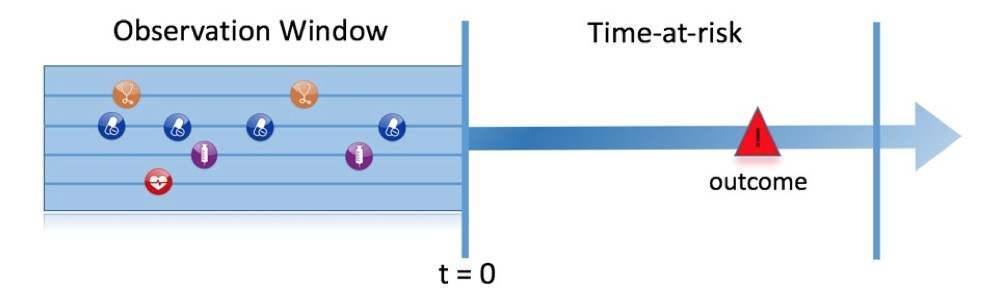
\includegraphics[width=1\linewidth]{images/PatientLevelPrediction/Figure1} \caption{The prediction problem}\label{fig:figure1}
\end{figure}

As shown in Figure \ref{fig:studydesign}, to define a prediction problem
we have to define t=0 by a Target Cohort (T), the outcome we like to
predict by an outcome cohort (O), and the time-at-risk (TAR).
Furthermore, we have to make design choices for the model we like to
develop, and determine the observational datasets to perform internal
and external validation. This conceptual framework works for all type of
prediction problems, for example those presented in Figure
\ref{fig:problems}.

\begin{figure}
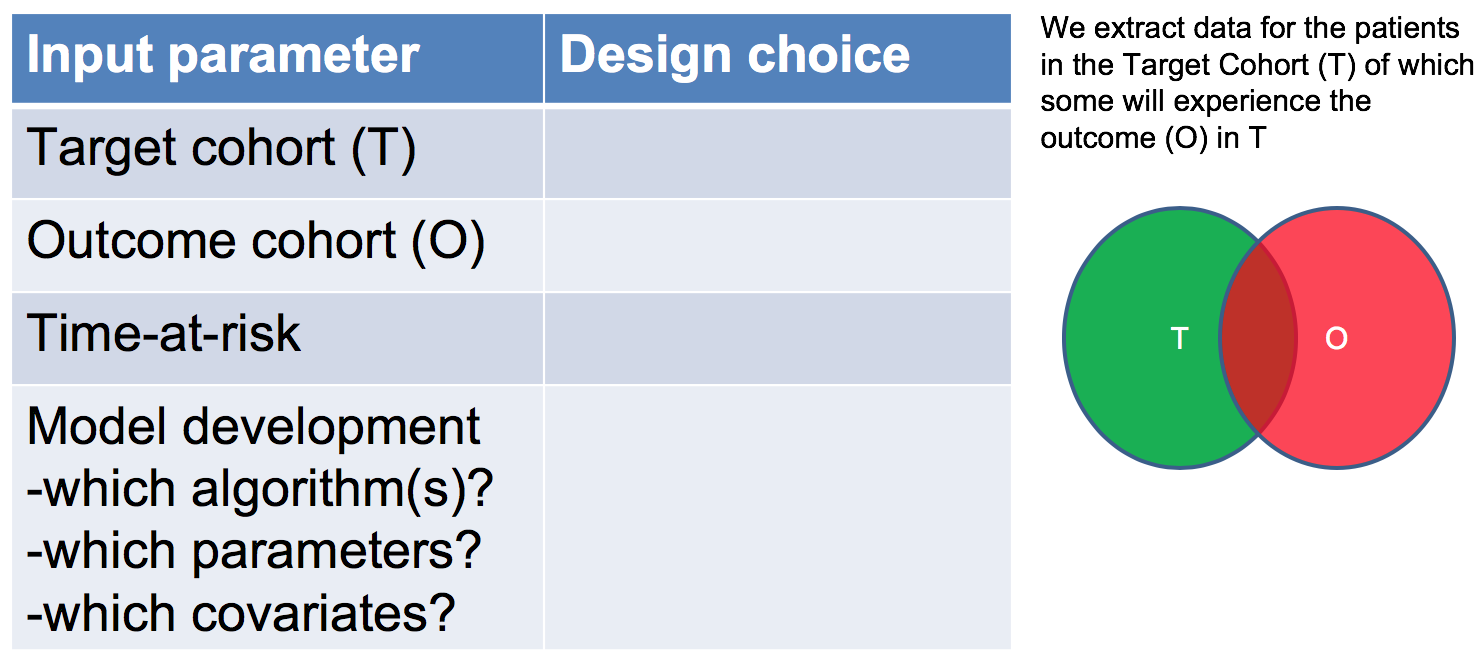
\includegraphics[width=1\linewidth]{images/PatientLevelPrediction/studydesign} \caption{Design choices}\label{fig:studydesign}
\end{figure}

\begin{figure}
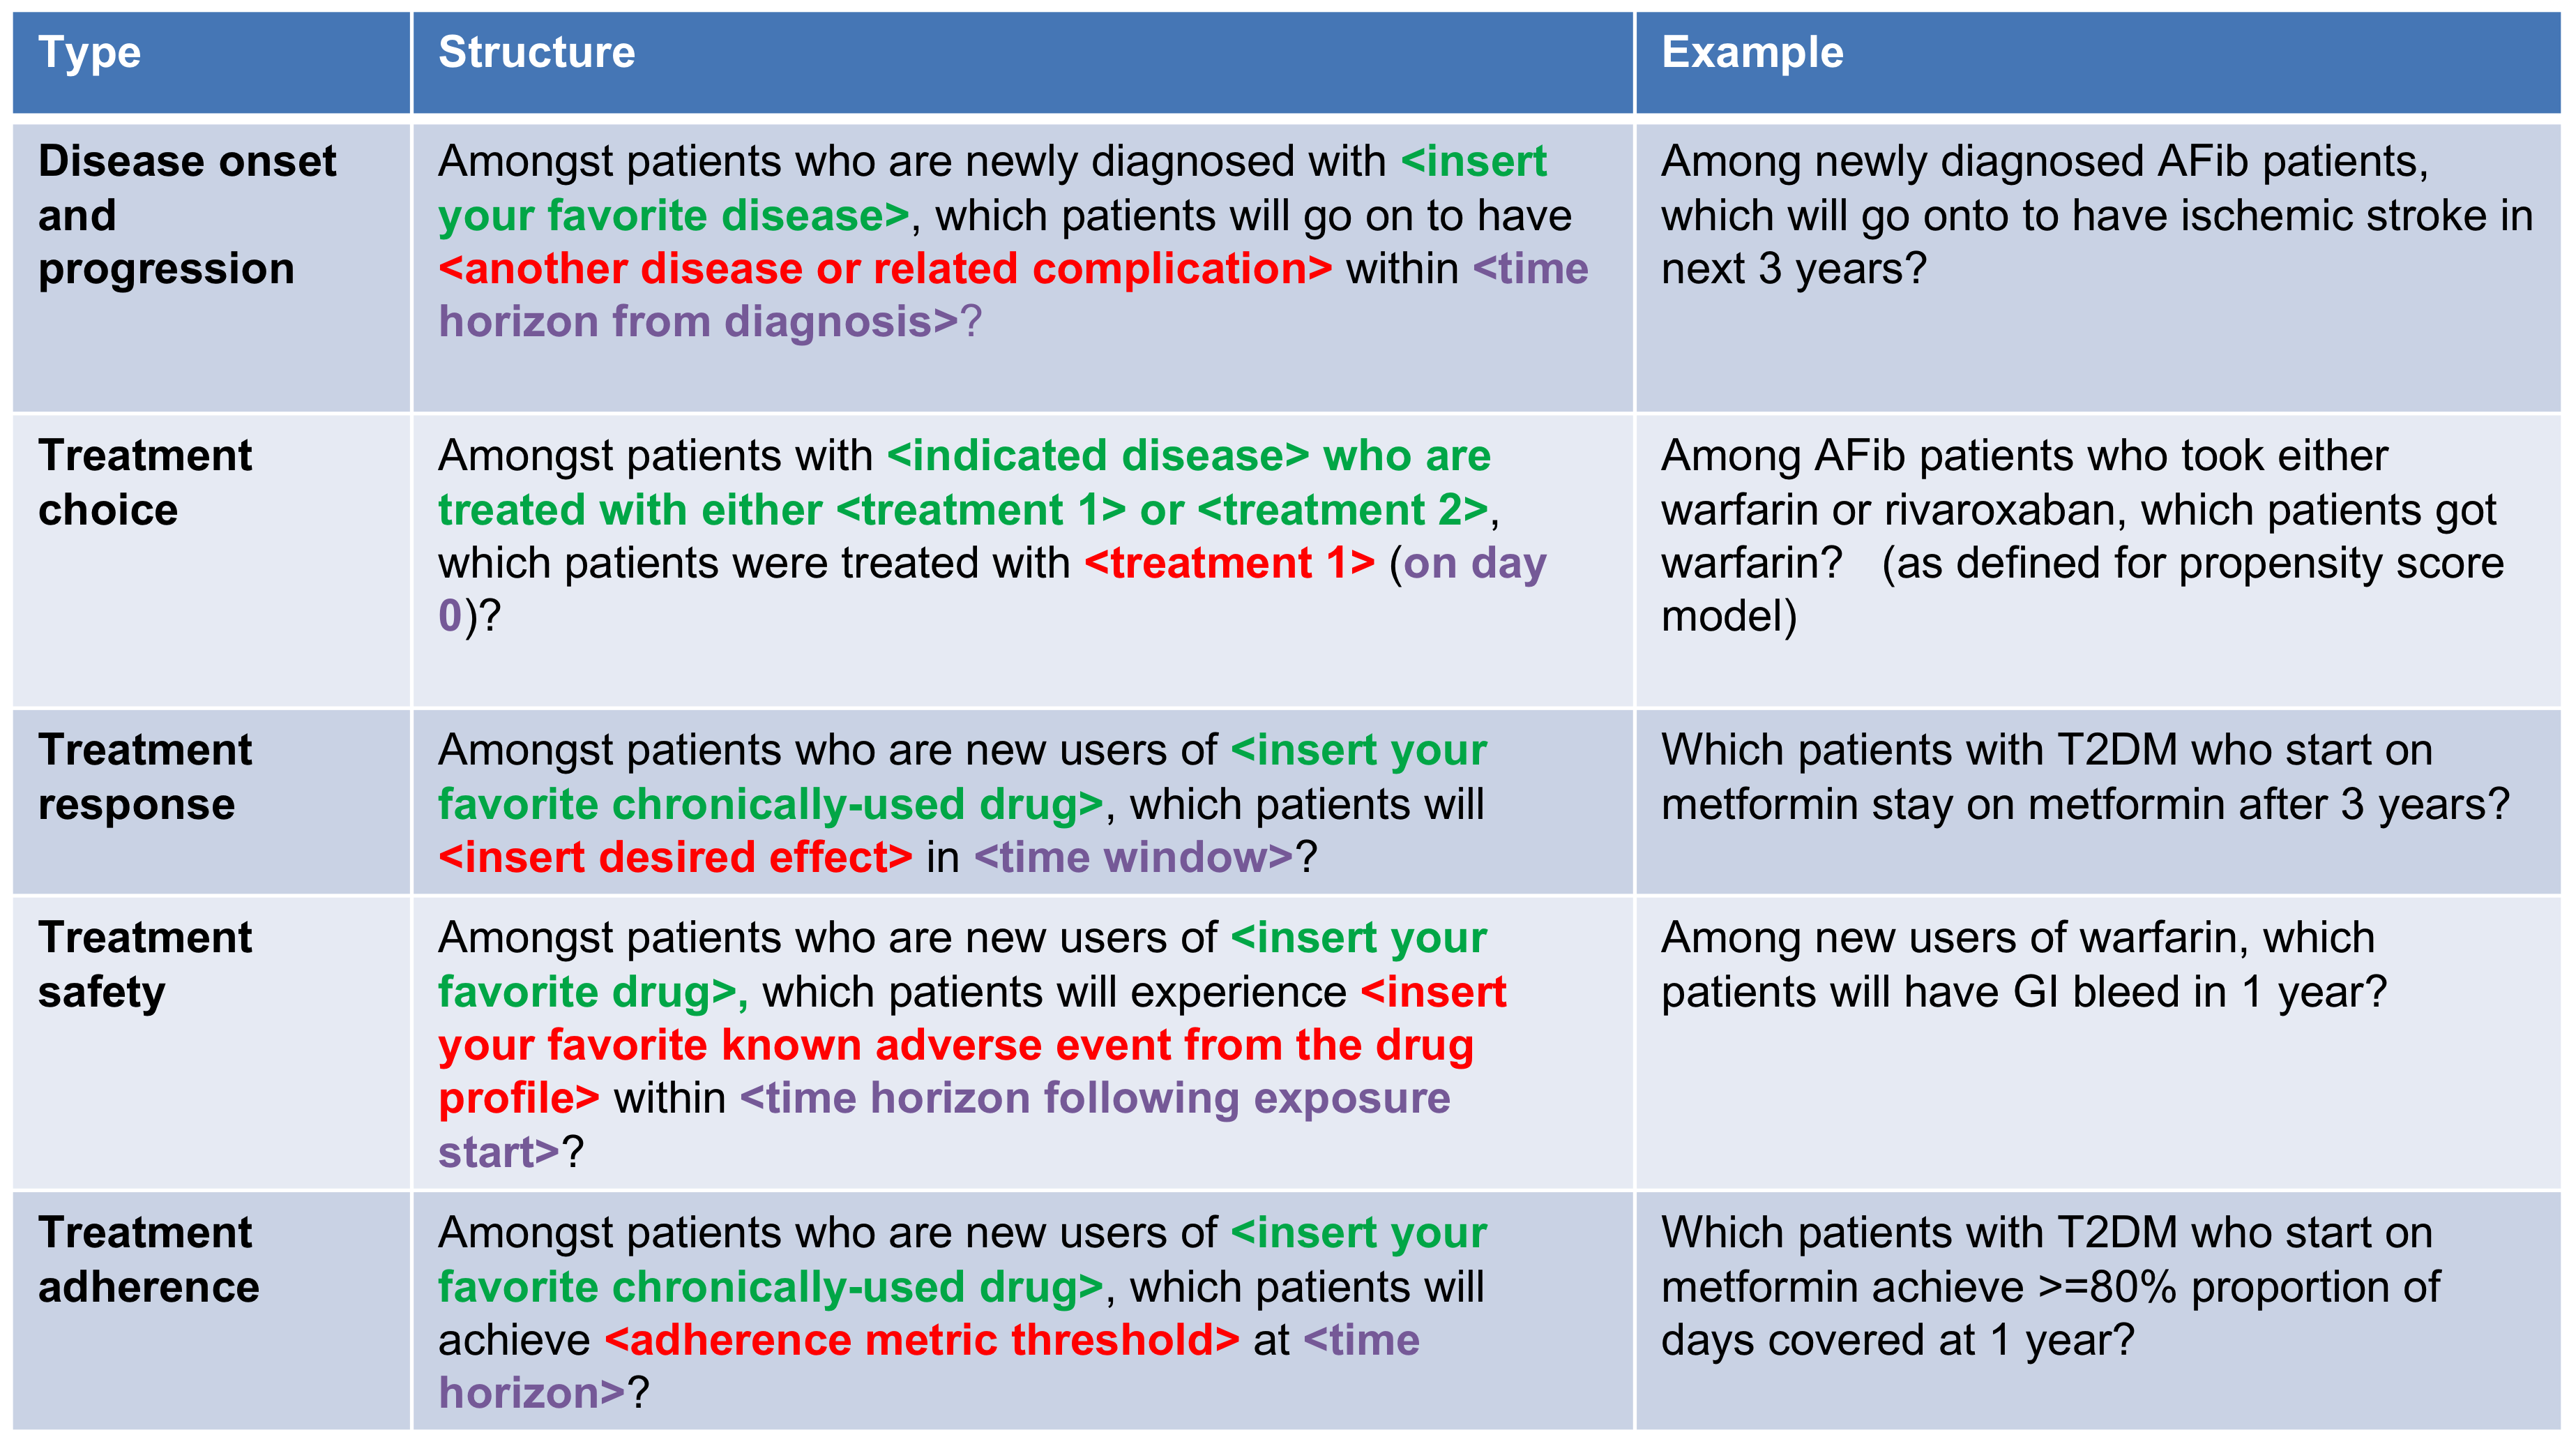
\includegraphics[width=1\linewidth]{images/PatientLevelPrediction/problems} \caption{Examples of prediction problems}\label{fig:problems}
\end{figure}

In the next sections we will explain the best practices for model
specification, implementation, and evaluation using OHDSI's
Patient-Level Prediction (PLP) framework as guidance.

\section{Study specification}\label{study-specification}

The first step is to clearly define the prediction problem.
Interestingly, in many published papers the prediction problem is poorly
defined, e.g., it is unclear how the index date (start of the Target
Cohort) is exactly defined. A poorly defined prediction problem does not
allow for external validation by others let alone implementation in
clinical practice. In the PLP framework we have enforced that we have to
define the prediction problem we like to address, in which population we
will build the model, which model we will build and how we will evaluate
its performance. In this section we will guide you through this process
and we will use a ``Disease onset and progression'' prediction type as
an example.

\subsection{Problem definition}\label{problem-definition}

Atrial fibrillation is a disease characterized by an irregular heart
rate that can cause poor blood flow. Patients with atrial fibrillation
are at increased risk of ischemic stroke. Anticoagulation is a
recommended prophylaxis treatment strategy for patients at high risk of
stroke, though the underuse of anticoagulants and persistent severity of
ischemic stroke represents a substantial unmet medical need. Various
strategies have been developed to predict risk of ischemic stroke in
patients with atrial fibrillation. CHADS2 \citep{gage2001} was developed
as a risk score based on history of congestive heart failure,
hypertension, age\textgreater{}=75, diabetes and stroke. CHADS2 was
initially derived using Medicare claims data, where it achieved good
discrimination (AUC=0.82). However, subsequent external validation
studies revealed the CHADS2 had substantially lower predictive accuracy
\citep{keogh2011}. Subsequent stroke risk calculators have been
developed and evaluated, including the extension of CHADS2Vasc. The
management of atrial fibrillation has evolved substantially over the
last decade, for various reasons that include the introduction of novel
oral anticoagulants. With these innovations has come a renewed interest
in greater precision medicine for stroke prevention.

We will apply the PLP framework to observational healthcare data to
address the following patient-level prediction question:

\begin{quote}
Amongst patients who are newly diagnosed with Atrial Fibrillation, which
patients will go on to have Ischemic Stroke within 1 year?
\end{quote}

We will define `patients who are newly diagnosed with Atrial
Fibrillation' as the first condition record of cardiac arrhythmia, which
is followed by another cardiac arrhythmia condition record, at least two
drug records for a drug used to treat arrhythmias, or a procedure to
treat arrhythmias. We will define `Ischemic stroke events' as ischemic
stroke condition records during an inpatient or ER visit; successive
records with \textgreater{} 180 day gap are considered independent
episodes.

\subsection{Study population
definition}\label{study-population-definition}

The final study population in which we will develop our model is often a
subset of the Target population, because we will e.g.~apply criteria
that are dependent on T and O or we want to do sensitivity analyses with
subpopulations of T. For this we have to answer the following questions:

\begin{itemize}
\item
  \emph{What is the minimum amount of observation time we require before
  the start of the target cohort?} This choice could depend on the
  available patient time in your training data, but also on the time you
  expect to be available in the data sources you want to apply the model
  on in the future. The longer the minimum observation time, the more
  baseline history time is available for each person to use for feature
  extraction, but the fewer patients will qualify for analysis.
  Moreover, there could be clinical reasons to choose a short or longer
  lookback period. For our example, we will use a prior history as
  lookback period (washout period).
\item
  \emph{Can patients enter the target cohort multiple times?} In the
  target cohort definition, a person may qualify for the cohort multiple
  times during different spans of time, for example if they had
  different episodes of a disease or separate periods of exposure to a
  medical product. The cohort definition does not necessarily apply a
  restriction to only let the patients enter once, but in the context of
  a particular patient-level prediction problem, a user may want to
  restrict the cohort to the first qualifying episode. In our example, a
  person could only enter the target cohort once since our criteria was
  based on first occurrence of atrial fibrillation.
\item
  \emph{Do we allow persons to enter the cohort if they experienced the
  outcome before?} Do we allow persons to enter the target cohort if
  they experienced the outcome before qualifying for the target cohort?
  Depending on the particular patient-level prediction problem, there
  may be a desire to predict `incident' first occurrence of an outcome,
  in which case patients who have previously experienced the outcome are
  not `at-risk' for having a first occurrence and therefore should be
  excluded from the target cohort. In other circumstances, there may be
  a desire to predict `prevalent' episodes, whereby patients with prior
  outcomes can be included in the analysis and the prior outcome itself
  can be a predictor of future outcomes. For our prediction example, the
  answer to this question is `Yes, allow persons with prior outcomes'
  because we know from the CHADS2 score that prior strokes are very
  predictive of future strokes. If this answer would have been `No' we
  also have to decide how long we would look back for previous
  occurrences of the outcome.
\item
  \emph{How do we define the period in which we will predict our outcome
  relative to the target cohort start?} We actually have to make two
  decisions to answer that question. First, does the time-at-risk window
  start at the date of the start of the target cohort or later?
  Arguments to make it start later could be that you want to avoid
  outcomes that were entered late in the record that actually occurred
  before the start of the target cohort or you want to leave a gap where
  interventions to prevent the outcome could theoretically be
  implemented. Second, you need to define the time-at-risk by setting
  the risk window end, as some specification of days offset relative to
  the target cohort start or end dates. For our problem we will predict
  in a `time-at-risk' window starting 1 day after the start of the
  target cohort up to 365 days later (to look for 1-year risk following
  atrial fibrillation diagnosis).
\item
  \emph{Do we require a minimum amount of time-at-risk?} We have to
  decide if we want to include patients that did not experience the
  outcome but did leave the database earlier than the end of our
  time-at-risk period. These patients may experience the outcome when we
  do not observe them. For our prediction problem we decide to answer
  this question with `Yes, require a mimimum time-at-risk' for that
  reason. Furthermore, we have to decide if this constraint also applies
  to persons who experienced the outcome or we will include all persons
  with the outcome irrespective of their total time at risk. For
  example, if the outcome is death, then persons with the outcome are
  likely censored before the full time-at-risk period is complete.
\end{itemize}

\subsection{Model development
settings}\label{model-development-settings}

To develop the model we have to decide which algorithm(s) we like to
train. We see the selection of the best algorithm for a certain
prediction problem as an empirical question, i.e.~you need to let the
data speak for itself and try different approaches to find the best one.
There is no algorithm that will work best for all problems (no free
lunch). In our framework we therefore aim to implement many algorithms.
Furthermore, we made the system modular so you can add your own custom
algorithms. This out-of-scope for this chapter but mode details can be
found in the AddingCustomAlgorithms vignette
(\url{https://github.com/OHDSI/PatientLevelPrediction/blob/master/inst/doc/AddingCustomAlgorithms.pdf}).

Our framework currently contains the following algorithms to choose
from:

\begin{longtable}[]{@{}lll@{}}
\toprule
\begin{minipage}[b]{0.12\columnwidth}\raggedright\strut
Algorithm\strut
\end{minipage} & \begin{minipage}[b]{0.55\columnwidth}\raggedright\strut
Description\strut
\end{minipage} & \begin{minipage}[b]{0.25\columnwidth}\raggedright\strut
Hyper-parameters\strut
\end{minipage}\tabularnewline
\midrule
\endhead
\begin{minipage}[t]{0.12\columnwidth}\raggedright\strut
Regularized Logistic Regression\strut
\end{minipage} & \begin{minipage}[t]{0.55\columnwidth}\raggedright\strut
Lasso logistic regression belongs to the family of generalized linear
models, where a linear combination of the variables is learned and
finally a logistic function maps the linear combination to a value
between 0 and 1. The lasso regularization adds a cost based on model
complexity to the objective function when training the model. This cost
is the sum of the absolute values of the linear combination of the
coefficients. The model automatically performs feature selection by
minimizing this cost. We use the Cyclic coordinate descent for logistic,
Poisson and survival analysis (Cyclops) package to perform large-scale
regularized logistic regression:
\url{https://github.com/OHDSI/Cyclops}\strut
\end{minipage} & \begin{minipage}[t]{0.25\columnwidth}\raggedright\strut
var (starting variance), seed\strut
\end{minipage}\tabularnewline
\begin{minipage}[t]{0.12\columnwidth}\raggedright\strut
Gradient boosting machines\strut
\end{minipage} & \begin{minipage}[t]{0.55\columnwidth}\raggedright\strut
Gradient boosting machines is a boosting ensemble technique and in our
framework it combines multiple decision trees. Boosting works by
iteratively adding decision trees but adds more weight to the
data-points that are misclassified by prior decision trees in the cost
function when training the next tree. We use Extreme Gradient Boosting,
which is an efficient implementation of the gradient boosting framework
implemented in the xgboost R package available from CRAN.\strut
\end{minipage} & \begin{minipage}[t]{0.25\columnwidth}\raggedright\strut
ntree (number of trees), max depth (max levels in tree), min rows
(minimum data points in in node), learning rate, seed\strut
\end{minipage}\tabularnewline
\begin{minipage}[t]{0.12\columnwidth}\raggedright\strut
Random forest\strut
\end{minipage} & \begin{minipage}[t]{0.55\columnwidth}\raggedright\strut
Random forest is a bagging ensemble technique that combines multiple
decision trees. The idea behind bagging is to reduce the likelihood of
overfitting, by using weak classifiers, but combining multiple diverse
weak classifiers into a strong classifier. Random forest accomplishes
this by training multiple decision trees but only using a subset of the
variables in each tree and the subset of variables differ between trees.
Our packages uses the sklearn learn implementation of Random Forest in
python.\strut
\end{minipage} & \begin{minipage}[t]{0.25\columnwidth}\raggedright\strut
mtry (number of features in each tree),ntree (number of trees), maxDepth
(max levels in tree), minRows (minimum data points in in node),balance
(balance class labels), seed\strut
\end{minipage}\tabularnewline
\begin{minipage}[t]{0.12\columnwidth}\raggedright\strut
K-nearest neighbors\strut
\end{minipage} & \begin{minipage}[t]{0.55\columnwidth}\raggedright\strut
K-nearest neighbors (KNN) is an algorithm that uses some metric to find
the K closest labelled data-points, given the specified metric, to a new
unlabelled data-point. The prediction of the new data-points is then the
most prevalent class of the K-nearest labelled data-points. There is a
sharing limitation of KNN, as the model requires labelled data to
perform the prediction on new data, and it is often not possible to
share this data across data sites.We included the BigKnn classifier
developed in OHDSI which is a large scale k-nearest neighbor classifier
using the Lucene search engine:
\url{https://github.com/OHDSI/BigKnn}\strut
\end{minipage} & \begin{minipage}[t]{0.25\columnwidth}\raggedright\strut
k (number of neighbours),weighted (weight by inverse frequency)\strut
\end{minipage}\tabularnewline
\begin{minipage}[t]{0.12\columnwidth}\raggedright\strut
Naive Bayes\strut
\end{minipage} & \begin{minipage}[t]{0.55\columnwidth}\raggedright\strut
The Naive Bayes algorithm applies the Bayes' theorem with the ``naive''
assumption of conditional independence between every pair of features
given the value of the class variable. Based on the likelihood the data
belongs to a class and the prior distribution of the class, a posterior
distribution is obtained.\strut
\end{minipage} & \begin{minipage}[t]{0.25\columnwidth}\raggedright\strut
none\strut
\end{minipage}\tabularnewline
\begin{minipage}[t]{0.12\columnwidth}\raggedright\strut
AdaBoost\strut
\end{minipage} & \begin{minipage}[t]{0.55\columnwidth}\raggedright\strut
AdaBoost is a boosting ensemble technique. Boosting works by iteratively
adding classifiers but adds more weight to the data-points that are
misclassified by prior classifiers in the cost function when training
the next classifier. We use the sklearn ``AdaboostClassifier''
implementation in Python.\strut
\end{minipage} & \begin{minipage}[t]{0.25\columnwidth}\raggedright\strut
nEstimators (the maximum number of estimators at which boosting is
terminated), learningRate (learning rate shrinks the contribution of
each classifier by learning\_rate. There is a trade-off between
learningRate and nEstimators)\strut
\end{minipage}\tabularnewline
\begin{minipage}[t]{0.12\columnwidth}\raggedright\strut
Decision Tree\strut
\end{minipage} & \begin{minipage}[t]{0.55\columnwidth}\raggedright\strut
A decision tree is a classifier that partitions the variable space using
individual tests selected using a greedy approach. It aims to find
partitions that have the highest information gain to separate the
classes. The decision tree can easily overfit by enabling a large number
of partitions (tree depth) and often needs some regularization (e.g.,
pruning or specifying hyper-parameters that limit the complexity of the
model). We use the sklearn ``DecisionTreeClassifier'' implementation in
Python.\strut
\end{minipage} & \begin{minipage}[t]{0.25\columnwidth}\raggedright\strut
maxDepth (the maximum depth of the tree),
minSamplesSplit,minSamplesLeaf, minImpuritySplit (threshold for early
stopping in tree growth. A node will split if its impurity is above the
threshold, otherwise it is a leaf.), seed,classWeight (``Balance''" or
``None'')\strut
\end{minipage}\tabularnewline
\begin{minipage}[t]{0.12\columnwidth}\raggedright\strut
Multilayer Perception\strut
\end{minipage} & \begin{minipage}[t]{0.55\columnwidth}\raggedright\strut
Neural networks contain multiple layers that weight their inputs using a
non-linear function. The first layer is the input layer, the last layer
is the output layer the between are the hidden layers. Neural networks
are generally trained using feed forward back-propagation. This is when
you go through the network with a data-point and calculate the error
between the true label and predicted label, then go backwards through
the network and update the linear function weights based on the error.
This can also be performed as a batch, where multiple data-points are
fee\strut
\end{minipage} & \begin{minipage}[t]{0.25\columnwidth}\raggedright\strut
size (the number of hidden nodes), alpha (the l2 regularisation),
seed\strut
\end{minipage}\tabularnewline
\begin{minipage}[t]{0.12\columnwidth}\raggedright\strut
Deep Learning\strut
\end{minipage} & \begin{minipage}[t]{0.55\columnwidth}\raggedright\strut
Deep learning such as deep nets, convolutional neural networks or
recurrent neural networks are similar to a neural network but have
multiple hidden layers that aim to learn latent representations useful
for prediction. In the seperate BuildingDeepLearningModels vignette we
describe these models and hyper-parameters in more detail\strut
\end{minipage} & \begin{minipage}[t]{0.25\columnwidth}\raggedright\strut
\strut
\end{minipage}\tabularnewline
\bottomrule
\end{longtable}

Furthermore, we have to decide on the \textbf{covariates} that we will
use to train our model. This choice can be driven by domain knowledge of
available computational resources. In our example, we like to add the
Gender, Age, Conditions, Drugs Groups, and Visit Count. We also have to
specify in which time windows we will look and we decide to look in year
before and any time prior.

\subsection{Model evaluation}\label{model-evaluation}

Finally, we have to define how we will train and test our model on our
data, i.e.~how we perform \textbf{internal validation}. For this we have
to decide how we divide our dataset in a training and testing dataset
and how we randomly assign patients to these two sets. Dependent on the
size of the training set we can decide how much data we like to use for
training, typically this is a 75\%, 25\% split. If you have very large
datasets you can use more data for training. To randomly assign patients
to the training and testing set, there are two commonly used approaches:

\begin{enumerate}
\def\labelenumi{\arabic{enumi}.}
\tightlist
\item
  split by person. In this case a random seed is used to assign the
  patient to either sets.
\item
  split by time. In this case a time point is used to split the persons,
  e.g.~75\% of the data is before and 25\% is after this date. The
  advantage of this is that you take into consideration that the health
  care system has changed over time.
\end{enumerate}

For our prediction model we decide to start with a Regularized Logistic
Regression and will use the default parameters. We will do a 75\%-25\%
split by person.

\subsection{Study summary}\label{study-summary}

We now completely defined our study:

\begin{longtable}[]{@{}ll@{}}
\toprule
\begin{minipage}[b]{0.42\columnwidth}\raggedright\strut
Definition\strut
\end{minipage} & \begin{minipage}[b]{0.51\columnwidth}\raggedright\strut
Value\strut
\end{minipage}\tabularnewline
\midrule
\endhead
\begin{minipage}[t]{0.42\columnwidth}\raggedright\strut
\textbf{Problem Definition}\strut
\end{minipage} & \begin{minipage}[t]{0.51\columnwidth}\raggedright\strut
\strut
\end{minipage}\tabularnewline
\begin{minipage}[t]{0.42\columnwidth}\raggedright\strut
Target Cohort (T)\strut
\end{minipage} & \begin{minipage}[t]{0.51\columnwidth}\raggedright\strut
`Patients who are newly diagnosed with Atrial Fibrillation' defined as
the first condition record of cardiac arrhythmia, which is followed by
another cardiac arrhythmia condition record, at least two drug records
for a drug used to treat arrhythmias, or a procedure to treat
arrhythmias.\strut
\end{minipage}\tabularnewline
\begin{minipage}[t]{0.42\columnwidth}\raggedright\strut
Outcome Cohort (O)\strut
\end{minipage} & \begin{minipage}[t]{0.51\columnwidth}\raggedright\strut
`Ischemic stroke events' defined as ischemic stroke condition records
during an inpatient or ER visit; successive records with \textgreater{}
180 day gap are considered independent episodes.\strut
\end{minipage}\tabularnewline
\begin{minipage}[t]{0.42\columnwidth}\raggedright\strut
Time-at-risk (TAR)\strut
\end{minipage} & \begin{minipage}[t]{0.51\columnwidth}\raggedright\strut
1 day till 365 days from cohort start\strut
\end{minipage}\tabularnewline
\begin{minipage}[t]{0.42\columnwidth}\raggedright\strut
\strut
\end{minipage} & \begin{minipage}[t]{0.51\columnwidth}\raggedright\strut
\strut
\end{minipage}\tabularnewline
\begin{minipage}[t]{0.42\columnwidth}\raggedright\strut
\textbf{Population Definition}\strut
\end{minipage} & \begin{minipage}[t]{0.51\columnwidth}\raggedright\strut
\strut
\end{minipage}\tabularnewline
\begin{minipage}[t]{0.42\columnwidth}\raggedright\strut
Washout Period\strut
\end{minipage} & \begin{minipage}[t]{0.51\columnwidth}\raggedright\strut
1095\strut
\end{minipage}\tabularnewline
\begin{minipage}[t]{0.42\columnwidth}\raggedright\strut
Enter the target cohort multiple times?\strut
\end{minipage} & \begin{minipage}[t]{0.51\columnwidth}\raggedright\strut
No\strut
\end{minipage}\tabularnewline
\begin{minipage}[t]{0.42\columnwidth}\raggedright\strut
Allow prior outcomes?\strut
\end{minipage} & \begin{minipage}[t]{0.51\columnwidth}\raggedright\strut
Yes\strut
\end{minipage}\tabularnewline
\begin{minipage}[t]{0.42\columnwidth}\raggedright\strut
Start of time-at-risk\strut
\end{minipage} & \begin{minipage}[t]{0.51\columnwidth}\raggedright\strut
1 day\strut
\end{minipage}\tabularnewline
\begin{minipage}[t]{0.42\columnwidth}\raggedright\strut
End of time-at-risk\strut
\end{minipage} & \begin{minipage}[t]{0.51\columnwidth}\raggedright\strut
365 days\strut
\end{minipage}\tabularnewline
\begin{minipage}[t]{0.42\columnwidth}\raggedright\strut
Require a minimum amount of time-at-risk?\strut
\end{minipage} & \begin{minipage}[t]{0.51\columnwidth}\raggedright\strut
Yes (364 days)\strut
\end{minipage}\tabularnewline
\begin{minipage}[t]{0.42\columnwidth}\raggedright\strut
\strut
\end{minipage} & \begin{minipage}[t]{0.51\columnwidth}\raggedright\strut
\strut
\end{minipage}\tabularnewline
\begin{minipage}[t]{0.42\columnwidth}\raggedright\strut
\textbf{Model Development}\strut
\end{minipage} & \begin{minipage}[t]{0.51\columnwidth}\raggedright\strut
\strut
\end{minipage}\tabularnewline
\begin{minipage}[t]{0.42\columnwidth}\raggedright\strut
Algorithm\strut
\end{minipage} & \begin{minipage}[t]{0.51\columnwidth}\raggedright\strut
Regularized Logistic Regression\strut
\end{minipage}\tabularnewline
\begin{minipage}[t]{0.42\columnwidth}\raggedright\strut
Hyper-parameters\strut
\end{minipage} & \begin{minipage}[t]{0.51\columnwidth}\raggedright\strut
variance = 0.01 (Default)\strut
\end{minipage}\tabularnewline
\begin{minipage}[t]{0.42\columnwidth}\raggedright\strut
Covariates\strut
\end{minipage} & \begin{minipage}[t]{0.51\columnwidth}\raggedright\strut
ender, Age, Conditions (ever before, \textless{}365), Drugs Groups (ever
before, \textless{}365), and Visit Count\strut
\end{minipage}\tabularnewline
\begin{minipage}[t]{0.42\columnwidth}\raggedright\strut
Data split\strut
\end{minipage} & \begin{minipage}[t]{0.51\columnwidth}\raggedright\strut
75\% train, 25\% test. Randomly assigned by person\strut
\end{minipage}\tabularnewline
\bottomrule
\end{longtable}

According to the best practices we need to make a protocol that
completely specifies how we plan to execute our study. This protocol
will be assessed by the governance boards of the participating data
sources in your network study. For this a template could be used but we
prefer to automate this process as much as possible by adding
functionality to automatically generate study protocol from a study
specification. We will discuss this in more detail later.

\section{Study implementation}\label{study-implementation}

Now we have completely design our study we have to implement the study.
This will be done using the
\href{http://github.com/OHDSI/PatientLevelPrediction}{\texttt{PatientLevelPrediction}}
package to build patient-level predictive models. The package enables
data extraction, model building, and model evaluation using data from
databases that are translated into the OMOP CDM. To install the package
we like to point you to the InstallationGuide that can be found on the
GitHub website (\url{https://github.com/OHDSI/PatientLevelPrediction/}).

We first have to generate the target and outcome cohorts and we then
need to develop the R code to run against our CDM to execute the full
study. These steps will be described in the paragraphs below.

\subsection{Cohort instantiation}\label{cohort-instantiation}

For our study we need to know when a person enters the target and
outcome cohorts. This is stored in a table on the server that contains
the cohort start date and cohort end date for all subjects for a
specific cohort definition. This cohort table has a very simple
structure as shown below:

\begin{itemize}
\tightlist
\item
  \texttt{cohort\_definition\_id}, a unique identifier for
  distinguishing between different types of cohorts, e.g.~cohorts of
  interest and outcome cohorts.
\item
  \texttt{subject\_id}, a unique identifier corresponding to the
  \texttt{person\_id} in the CDM.
\item
  \texttt{cohort\_start\_date}, the date the subject enters the cohort.
\item
  \texttt{cohort\_end\_date}, the date the subject leaves the cohort.
\end{itemize}

How do we fill this table according to our cohort definitions? There are
two options for this:

\begin{enumerate}
\def\labelenumi{\arabic{enumi})}
\item
  use the interactive cohort builder tool in ATLAS
  (www.github.com/OHDSI/ATLAS) which can be used to create cohorts based
  on inclusion criteria and will automatically populate this cohort
  table.
\item
  write your own custom SQL statements to fill the cohort table.
\end{enumerate}

Both methods are described below for our example prediction problem.

\subsubsection{ATLAS cohort builder}\label{atlas-cohort-builder}

\begin{figure}
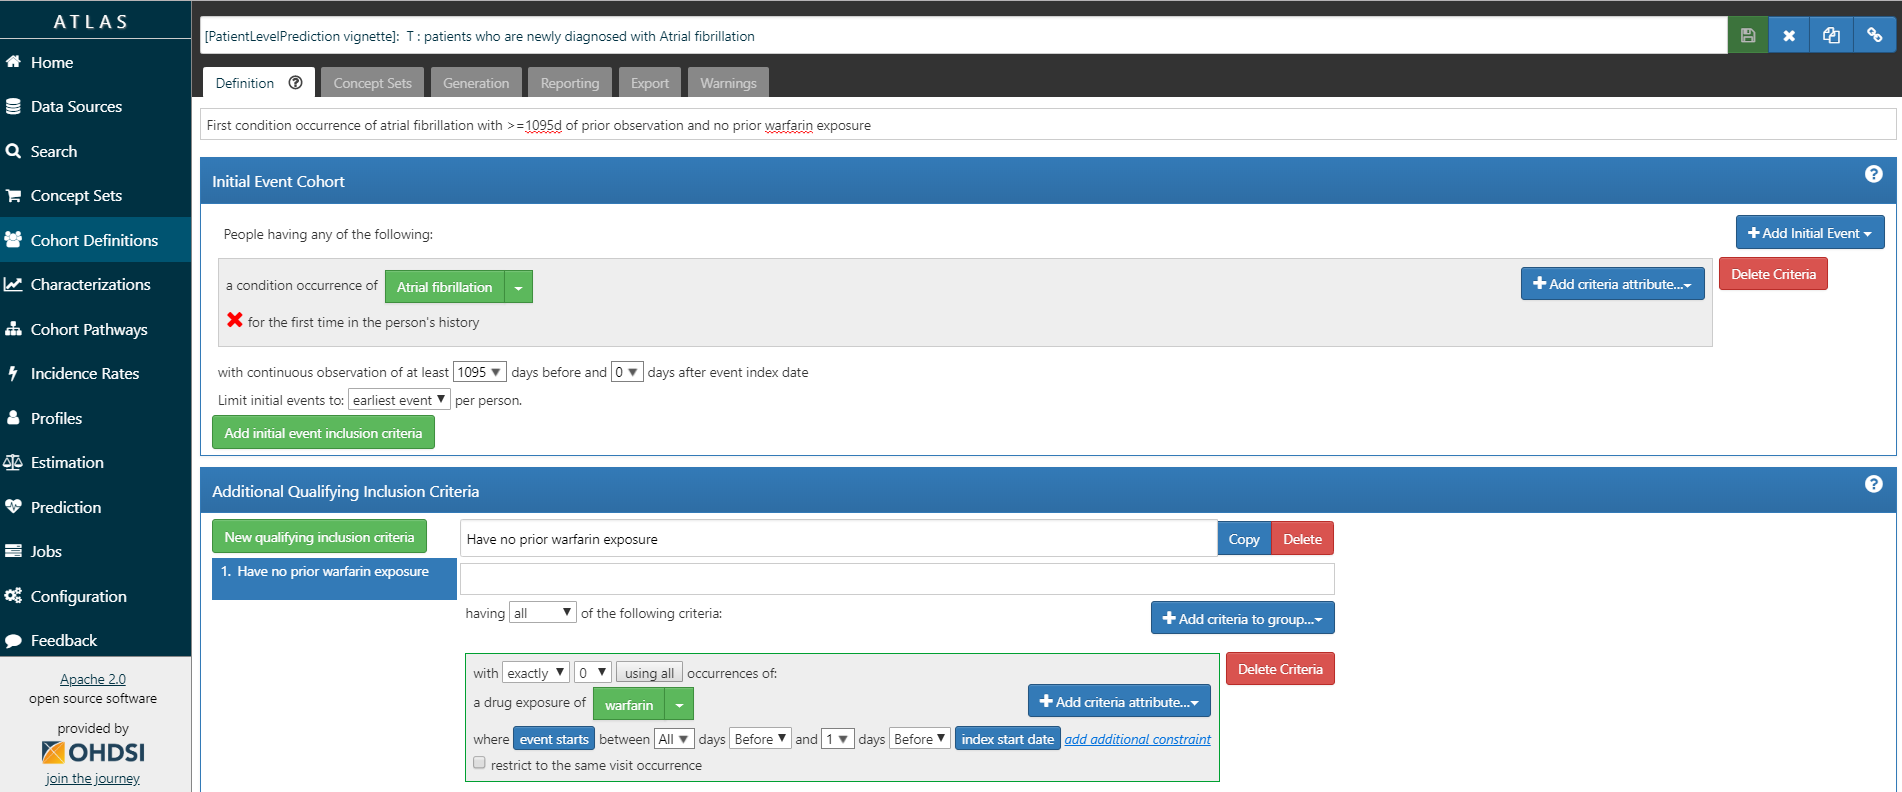
\includegraphics[width=1\linewidth]{images/PatientLevelPrediction/atlast} \caption{Target Cohort Atrial Fibrillation}\label{fig:atlast}
\end{figure}

ATLAS allows you to define cohorts interactively by specifying cohort
entry and cohort exit criteria. Cohort entry criteria involve selecting
one or more initial events, which determine the start date for cohort
entry, and optionally specifying additional inclusion criteria which
filter to the qualifying events. Cohort exit criteria are applied to
each cohort entry record to determine the end date when the person's
episode no longer qualifies for the cohort. For the outcome cohort the
end date is less relevant. As an example, Figure \ref{fig:atlast} shows
how we created the Atrial Fibrillation cohort and Figure
\ref{fig:atlaso} shows how we created the stroke cohort in ATLAS.

\begin{figure}
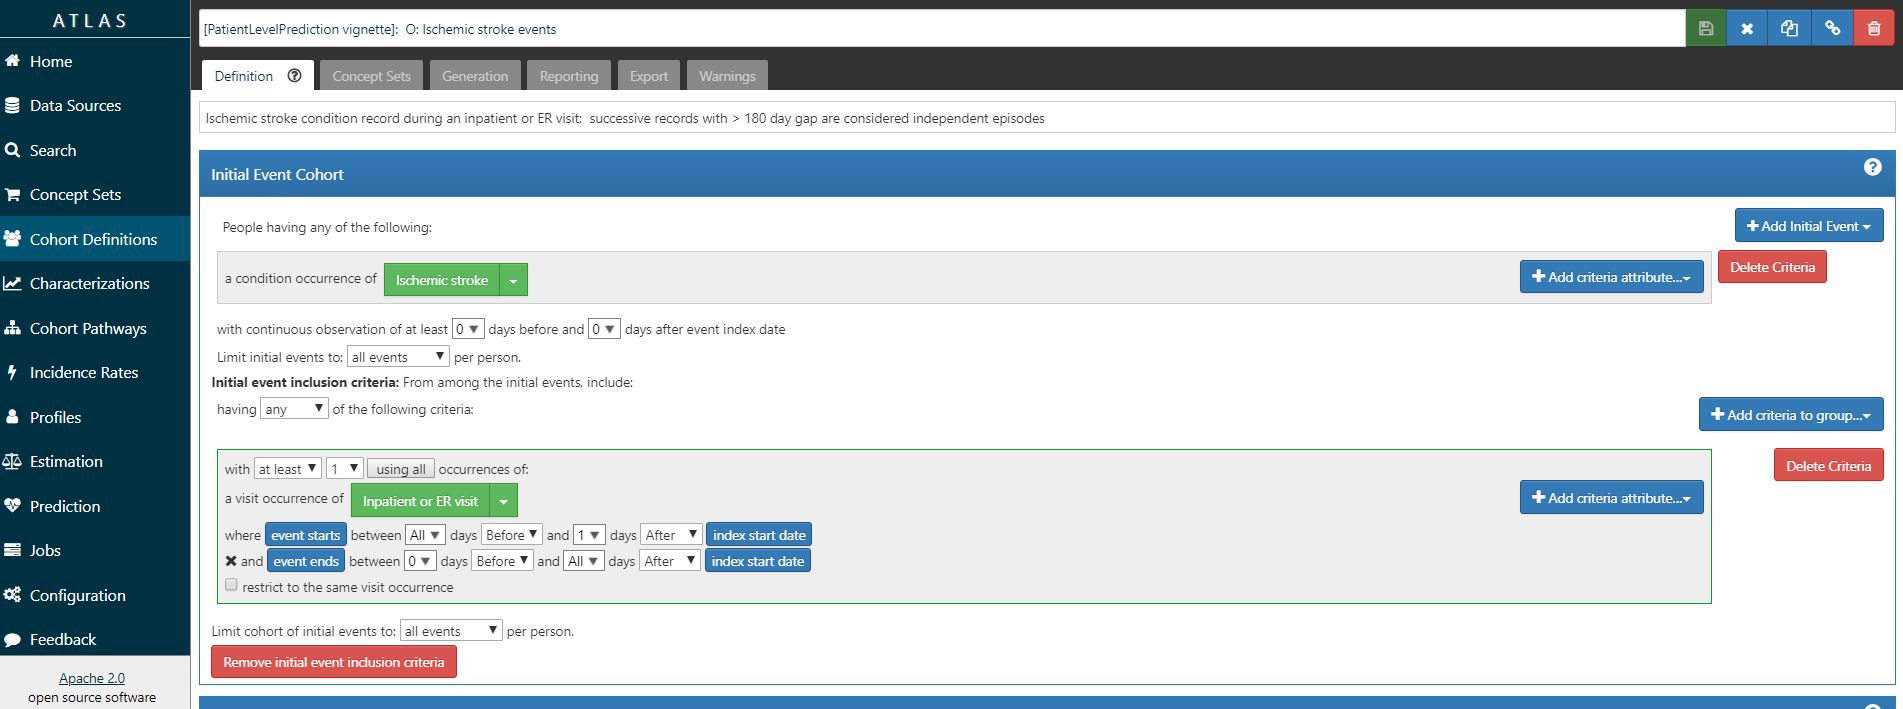
\includegraphics[width=1\linewidth]{images/PatientLevelPrediction/atlaso} \caption{Outcome Cohort Stroke}\label{fig:atlaso}
\end{figure}

The T and O cohorts can be found here:

\begin{itemize}
\tightlist
\item
  Atrial Fibrillaton (T):
  \url{http://www.ohdsi.org/web/atlas/\#/cohortdefinition/1769447}
\item
  Stroke (O) :
  \url{http://www.ohdsi.org/web/atlas/\#/cohortdefinition/1769448}
\end{itemize}

In depth explanation of cohort creation in ATLAS is out of scope of this
vignette but can be found on the OHDSI wiki pages
(\url{http://www.ohdsi.org/web/wiki/doku.php?id=documentation:software:atlas}).

Note that when a cohort is created in ATLAS the cohortid is needed to
extract the data in R. The cohortid can be found at the top of the ATLAS
screen.

\subsubsection{Custom cohorts}\label{custom-cohorts}

It is also possible to create cohorts without the use of ATLAS. Using
custom cohort code (SQL) you can make more advanced cohorts if needed.

For our example study, we need to create at table to hold the cohort
data and we need to create SQL code to instantiate this table for both
the AF and Stroke cohorts. Therefore, we create a file called
\emph{AfStrokeCohorts.sql} with the following contents:

\begin{Shaded}
\begin{Highlighting}[]
\CommentTok{/***********************************}
\CommentTok{File AfStrokeCohorts.sql}
\CommentTok{***********************************/}
\CommentTok{/*}
\CommentTok{  Create a table to store the persons in the T and C cohort}
\CommentTok{*/}

\KeywordTok{IF}\NormalTok{ OBJECT_ID(}\StringTok{'@resultsDatabaseSchema.PLPAFibStrokeCohort'}\NormalTok{, }\StringTok{'U'}\NormalTok{) }\KeywordTok{IS} \KeywordTok{NOT} \KeywordTok{NULL}
  \KeywordTok{DROP} \KeywordTok{TABLE}\NormalTok{ @resultsDatabaseSchema.PLPAFibStrokeCohort;}

\KeywordTok{CREATE} \KeywordTok{TABLE}\NormalTok{ @resultsDatabaseSchema.PLPAFibStrokeCohort}
\NormalTok{(}
\NormalTok{  cohort_definition_id }\DataTypeTok{INT}\NormalTok{,}
\NormalTok{  subject_id BIGINT,}
\NormalTok{  cohort_start_date }\DataTypeTok{DATE}\NormalTok{,}
\NormalTok{  cohort_end_date }\DataTypeTok{DATE}
\NormalTok{);}


\CommentTok{/*}
\CommentTok{  T cohort:  [PatientLevelPrediction vignette]:  T : patients who are newly}
\CommentTok{             diagnosed with Atrial fibrillation}
\CommentTok{  - persons with a condition occurrence record of 'Atrial fibrillation' or}
\CommentTok{    any descendants, indexed at the first diagnosis}
\CommentTok{  - who have >1095 days of prior observation before their first diagnosis}
\CommentTok{  - and have no warfarin exposure any time prior to first AFib diagnosis}
\CommentTok{*/}
\KeywordTok{INSERT} \KeywordTok{INTO}\NormalTok{ @resultsDatabaseSchema.AFibStrokeCohort (cohort_definition_id,}
\NormalTok{                                                     subject_id,}
\NormalTok{                                                     cohort_start_date,}
\NormalTok{                                                     cohort_end_date)}
\KeywordTok{SELECT} \DecValTok{1} \KeywordTok{AS}\NormalTok{ cohort_definition_id,}
\NormalTok{  AFib.person_id }\KeywordTok{AS}\NormalTok{ subject_id,}
\NormalTok{  AFib.condition_start_date }\KeywordTok{AS}\NormalTok{ cohort_start_date,}
\NormalTok{  observation_period.observation_period_end_date }\KeywordTok{AS}\NormalTok{ cohort_end_date}
\KeywordTok{FROM}
\NormalTok{(}
  \KeywordTok{SELECT}\NormalTok{ person_id, }\FunctionTok{min}\NormalTok{(condition_start_date) }\KeywordTok{as}\NormalTok{ condition_start_date}
  \KeywordTok{FROM}\NormalTok{ @cdmDatabaseSchema.condition_occurrence}
  \KeywordTok{WHERE}\NormalTok{ condition_concept_id }\KeywordTok{IN}\NormalTok{ (}\KeywordTok{SELECT}\NormalTok{ descendant_concept_id }\KeywordTok{FROM}
\NormalTok{        @cdmDatabaseSchema.concept_ancestor }\KeywordTok{WHERE}\NormalTok{ ancestor_concept_id }\KeywordTok{IN}
\NormalTok{        (}\DecValTok{313217} \CommentTok{/*atrial fibrillation*/}\NormalTok{))}
  \KeywordTok{GROUP} \KeywordTok{BY}\NormalTok{ person_id}
\NormalTok{) AFib}
\KeywordTok{INNER} \KeywordTok{JOIN}\NormalTok{ @cdmDatabaseSchema.observation_period}
  \KeywordTok{ON}\NormalTok{ AFib.person_id = observation_period.person_id}
  \KeywordTok{AND}\NormalTok{ AFib.condition_start_date >= dateadd(dd,}\DecValTok{1095}\NormalTok{,}
\NormalTok{                                   observation_period.observation_period_start_date)}
  \KeywordTok{AND}\NormalTok{ AFib.condition_start_date <= observation_period.observation_period_end_date}
\KeywordTok{LEFT} \KeywordTok{JOIN}
\NormalTok{(}
  \KeywordTok{SELECT}\NormalTok{ person_id, }\FunctionTok{min}\NormalTok{(drug_exposure_start_date) }\KeywordTok{as}\NormalTok{ drug_exposure_start_date}
  \KeywordTok{FROM}\NormalTok{ @cdmDatabaseSchema.drug_exposure}
  \KeywordTok{WHERE}\NormalTok{ drug_concept_id }\KeywordTok{IN}\NormalTok{ (}\KeywordTok{SELECT}\NormalTok{ descendant_concept_id }\KeywordTok{FROM}
\NormalTok{       @cdmDatabaseSchema.concept_ancestor }\KeywordTok{WHERE}\NormalTok{ ancestor_concept_id }\KeywordTok{IN}
\NormalTok{       (}\DecValTok{1310149} \CommentTok{/*warfarin*/}\NormalTok{))}
  \KeywordTok{GROUP} \KeywordTok{BY}\NormalTok{ person_id}
\NormalTok{) warfarin}
  \KeywordTok{ON}\NormalTok{ Afib.person_id = warfarin.person_id}
  \KeywordTok{AND}\NormalTok{ Afib.condition_start_date > warfarin.drug_exposure_start_date}
\KeywordTok{WHERE}\NormalTok{ warfarin.person_id }\KeywordTok{IS} \KeywordTok{NULL}
\NormalTok{;}

\CommentTok{/*}
\CommentTok{  C cohort:  [PatientLevelPrediction vignette]:  O: Ischemic stroke events}
\CommentTok{  - inpatient visits that include a condition occurrence record for}
\CommentTok{    'cerebral infarction' and descendants, 'cerebral thrombosis',}
\CommentTok{    'cerebral embolism', 'cerebral artery occlusion'}
\CommentTok{*/}
\KeywordTok{INSERT} \KeywordTok{INTO}\NormalTok{ @resultsDatabaseSchema.AFibStrokeCohort (cohort_definition_id,}
\NormalTok{                                                     subject_id,}
\NormalTok{                                                     cohort_start_date,}
\NormalTok{                                                     cohort_end_date)}
\KeywordTok{SELECT} \DecValTok{2} \KeywordTok{AS}\NormalTok{ cohort_definition_id,}
\NormalTok{  visit_occurrence.person_id }\KeywordTok{AS}\NormalTok{ subject_id,}
\NormalTok{  visit_occurrence.visit_start_date }\KeywordTok{AS}\NormalTok{ cohort_start_date,}
\NormalTok{  visit_occurrence.visit_end_date }\KeywordTok{AS}\NormalTok{ cohort_end_date}
\KeywordTok{FROM}
\NormalTok{(}
  \KeywordTok{SELECT}\NormalTok{ person_id, condition_start_date}
  \KeywordTok{FROM}\NormalTok{ @cdmDatabaseSchema.condition_occurrence}
  \KeywordTok{WHERE}\NormalTok{ condition_concept_id }\KeywordTok{IN}\NormalTok{ (}\KeywordTok{SELECT} \KeywordTok{DISTINCT}\NormalTok{ descendant_concept_id }\KeywordTok{FROM}
\NormalTok{  @cdmDatabaseSchema.concept_ancestor }\KeywordTok{WHERE}\NormalTok{ ancestor_concept_id }\KeywordTok{IN}
\NormalTok{  (}\DecValTok{443454} \CommentTok{/*cerebral infarction*/}\NormalTok{) }\KeywordTok{OR}\NormalTok{ descendant_concept_id }\KeywordTok{IN}
\NormalTok{  (}\DecValTok{441874} \CommentTok{/*cerebral thrombosis*/}\NormalTok{, }\DecValTok{375557} \CommentTok{/*cerebral embolism*/}\NormalTok{,}
   \DecValTok{372924} \CommentTok{/*cerebral artery occlusion*/}\NormalTok{))}
\NormalTok{) stroke}
\KeywordTok{INNER} \KeywordTok{JOIN}\NormalTok{ @cdmDatabaseSchema.visit_occurrence}
\KeywordTok{ON}\NormalTok{ stroke.person_id = visit_occurrence.person_id}
\KeywordTok{AND}\NormalTok{ stroke.condition_start_date >= visit_occurrence.visit_start_date}
\KeywordTok{AND}\NormalTok{ stroke.condition_start_date <= visit_occurrence.visit_end_date}
\KeywordTok{AND}\NormalTok{ visit_occurrence.visit_concept_id }\KeywordTok{IN}\NormalTok{ (}\DecValTok{9201}\NormalTok{, }\DecValTok{262} \CommentTok{/*'Inpatient Visit'  or}
\CommentTok{    'Emergency Room and Inpatient Visit'*/}\NormalTok{)}
\KeywordTok{GROUP} \KeywordTok{BY}\NormalTok{ visit_occurrence.person_id, visit_occurrence.visit_start_date,}
\NormalTok{         visit_occurrence.visit_end_date}
\NormalTok{;}
\end{Highlighting}
\end{Shaded}

This is parameterized SQL which can be used by the
\href{http://github.com/OHDSI/SqlRender}{\texttt{SqlRender}} package. We
use parameterized SQL so we do not have to pre-specify the names of the
CDM and result schemas. That way, if we want to run the SQL on a
different schema, we only need to change the parameter values; we do not
have to change the SQL code. By also making use of translation
functionality in \texttt{SqlRender}, we can make sure the SQL code can
be run in many different environments.

To execute this SQL against our CDM we first need to tell R how to
connect to the server.
\href{http://github.com/OHDSI/PatientLevelPrediction}{\texttt{PatientLevelPrediction}}
uses the
\href{http://github.com/ohdsi/DatabaseConnector}{\texttt{DatabaseConnector}}
package, which provides a function called
\texttt{createConnectionDetails}. Type \texttt{?createConnectionDetails}
for the specific settings required for the various database management
systems (DBMS). For example, one might connect to a PostgreSQL database
using this code:

\begin{Shaded}
\begin{Highlighting}[]
\NormalTok{connectionDetails <-}\StringTok{ }\KeywordTok{createConnectionDetails}\NormalTok{(}\DataTypeTok{dbms =} \StringTok{"postgresql"}\NormalTok{,}
                                             \DataTypeTok{server =} \StringTok{"localhost/ohdsi"}\NormalTok{,}
                                             \DataTypeTok{user =} \StringTok{"joe"}\NormalTok{,}
                                             \DataTypeTok{password =} \StringTok{"supersecret"}\NormalTok{)}

\NormalTok{cdmDatabaseSchema <-}\StringTok{ "my_cdm_data"}
\NormalTok{cohortsDatabaseSchema <-}\StringTok{ "my_results"}
\NormalTok{cdmVersion <-}\StringTok{ "5"}
\end{Highlighting}
\end{Shaded}

The last three lines define the \texttt{cdmDatabaseSchema} and
\texttt{cohortsDatabaseSchema} variables, as well as the CDM version. We
will use these later to tell R where the data in CDM format live, where
we want to create the cohorts of interest, and what version CDM is used.
Note that for Microsoft SQL Server, databaseschemas need to specify both
the database and the schema, so for example
\texttt{cdmDatabaseSchema\ \textless{}-\ "my\_cdm\_data.dbo"}.

\begin{Shaded}
\begin{Highlighting}[]
\KeywordTok{library}\NormalTok{(SqlRender)}
\NormalTok{sql <-}\StringTok{ }\KeywordTok{readSql}\NormalTok{(}\StringTok{"AfStrokeCohorts.sql"}\NormalTok{)}
\NormalTok{sql <-}\StringTok{ }\KeywordTok{renderSql}\NormalTok{(sql,}
\DataTypeTok{cdmDatabaseSchema =}\NormalTok{ cdmDatabaseSchema,}
\DataTypeTok{cohortsDatabaseSchema =}\NormalTok{ cohortsDatabaseSchema,}
\DataTypeTok{post_time =} \DecValTok{30}\NormalTok{,}
\DataTypeTok{pre_time =} \DecValTok{365}\NormalTok{)}\OperatorTok{$}\NormalTok{sql}
\NormalTok{sql <-}\StringTok{ }\KeywordTok{translateSql}\NormalTok{(sql, }\DataTypeTok{targetDialect =}\NormalTok{ connectionDetails}\OperatorTok{$}\NormalTok{dbms)}\OperatorTok{$}\NormalTok{sql}

\NormalTok{connection <-}\StringTok{ }\KeywordTok{connect}\NormalTok{(connectionDetails)}
\KeywordTok{executeSql}\NormalTok{(connection, sql)}
\end{Highlighting}
\end{Shaded}

In this code, we first read the SQL from the file into memory. In the
next line, we replace four parameter names with the actual values. We
then translate the SQL into the dialect appropriate for the DBMS we
already specified in the \texttt{connectionDetails}. Next, we connect to
the server, and submit the rendered and translated SQL.

If all went well, we now have a table with the events of interest. We
can see how many events per type:

\begin{Shaded}
\begin{Highlighting}[]
\NormalTok{sql <-}\StringTok{ }\KeywordTok{paste}\NormalTok{(}\StringTok{"SELECT cohort_definition_id, COUNT(*) AS count"}\NormalTok{,}
\StringTok{"FROM @cohortsDatabaseSchema.AFibStrokeCohort"}\NormalTok{,}
\StringTok{"GROUP BY cohort_definition_id"}\NormalTok{)}
\NormalTok{sql <-}\StringTok{ }\KeywordTok{renderSql}\NormalTok{(sql, }\DataTypeTok{cohortsDatabaseSchema =}\NormalTok{ cohortsDatabaseSchema)}\OperatorTok{$}\NormalTok{sql}
\NormalTok{sql <-}\StringTok{ }\KeywordTok{translateSql}\NormalTok{(sql, }\DataTypeTok{targetDialect =}\NormalTok{ connectionDetails}\OperatorTok{$}\NormalTok{dbms)}\OperatorTok{$}\NormalTok{sql}

\KeywordTok{querySql}\NormalTok{(connection, sql)}
\end{Highlighting}
\end{Shaded}

\begin{verbatim}
##   cohort_definition_id  count
## 1                    1 527616
## 2                    2 221555
\end{verbatim}

\subsection{Study script creation}\label{study-script-creation}

In this section we assume that our cohorts have been created either by
using ATLAS or a custom SQL script. We will first explain how to create
an R script yourself that will execute our study as we have defined
earlier.

\subsubsection{Data extraction}\label{data-extraction}

Now we can tell
\href{http://github.com/OHDSI/PatientLevelPrediction}{\texttt{PatientLevelPrediction}}
to extract all necessary data for our analysis. This is done using the
FeatureExtractionPackage package
(\url{https://github.com/OHDSI/FeatureExtration}). In short the
FeatureExtractionPackage allows you to specify which features
(covariates) need to be extracted, e.g.~all conditions and drug
exposures, more information can be found in chapter X. It also supports
the creation of custom covariates. For more detailed information on the
FeatureExtraction package see its vignettes. For our example study we
decided to use these settings:

\begin{Shaded}
\begin{Highlighting}[]
\NormalTok{covariateSettings <-}\StringTok{ }\KeywordTok{createCovariateSettings}\NormalTok{(}\DataTypeTok{useDemographicsGender =} \OtherTok{TRUE}\NormalTok{,}
                                             \DataTypeTok{useDemographicsAge =} \OtherTok{TRUE}\NormalTok{,}
                                             \DataTypeTok{useConditionGroupEraLongTerm =} \OtherTok{TRUE}\NormalTok{,}
                                             \DataTypeTok{useConditionGroupEraAnyTimePrior =} \OtherTok{TRUE}\NormalTok{,}
                                             \DataTypeTok{useDrugGroupEraLongTerm =} \OtherTok{TRUE}\NormalTok{,}
                                             \DataTypeTok{useDrugGroupEraAnyTimePrior =} \OtherTok{TRUE}\NormalTok{,}
                                             \DataTypeTok{useVisitConceptCountLongTerm =} \OtherTok{TRUE}\NormalTok{,}
                                             \DataTypeTok{longTermStartDays =} \OperatorTok{-}\DecValTok{365}\NormalTok{,}
                                             \DataTypeTok{endDays =} \OperatorTok{-}\DecValTok{1}\NormalTok{)}
\end{Highlighting}
\end{Shaded}

The final step for extracting the data is to run the \texttt{getPlpData}
function and input the connection details, the database schema where the
cohorts are stored, the cohort definition ids for the cohort and
outcome, and the washoutPeriod which is the minimum number of days prior
to cohort index date that the person must have been observed to be
included into the data, and finally input the previously constructed
covariate settings.

\begin{Shaded}
\begin{Highlighting}[]
\NormalTok{plpData <-}\StringTok{ }\KeywordTok{getPlpData}\NormalTok{(}\DataTypeTok{connectionDetails =}\NormalTok{ connectionDetails,}
                      \DataTypeTok{cdmDatabaseSchema =}\NormalTok{ cdmDatabaseSchema,}
                      \DataTypeTok{cohortDatabaseSchema =}\NormalTok{ resultsDatabaseSchema,}
                      \DataTypeTok{cohortTable =} \StringTok{'AFibStrokeCohort'}\NormalTok{,}
                      \DataTypeTok{cohortId =} \DecValTok{1}\NormalTok{,}
                      \DataTypeTok{covariateSettings =}\NormalTok{ covariateSettings,}
                      \DataTypeTok{outcomeDatabaseSchema =}\NormalTok{ resultsDatabaseSchema,}
                      \DataTypeTok{outcomeTable =} \StringTok{'AFibStrokeCohort'}\NormalTok{,}
                      \DataTypeTok{outcomeIds =} \DecValTok{2}\NormalTok{,}
                      \DataTypeTok{sampleSize =} \DecValTok{10000}
\NormalTok{)}
\end{Highlighting}
\end{Shaded}

Note that if the cohorts are created in ATLAS its corresponding cohort
database schema needs to be selected. There are many additional
parameters for the \texttt{getPlpData} function which are all documented
in the
\href{http://github.com/OHDSI/PatientLevelPrediction}{\texttt{PatientLevelPrediction}}
manual. The resulting \texttt{plpData} object uses the package
\texttt{ff} to store information in a way that ensures R does not run
out of memory, even when the data are large.

Creating the \texttt{plpData} object can take considerable computing
time, and it is probably a good idea to save it for future sessions.
Because \texttt{plpData} uses \texttt{ff}, we cannot use R's regular
save function. Instead, we'll have to use the \texttt{savePlpData()}
function:

\begin{Shaded}
\begin{Highlighting}[]
\KeywordTok{savePlpData}\NormalTok{(plpData, }\StringTok{"stroke_in_af_data"}\NormalTok{)}
\end{Highlighting}
\end{Shaded}

We can use the \texttt{loadPlpData()} function to load the data in a
future session.

\subsubsection{Additional inclusion
criteria}\label{additional-inclusion-criteria}

To completely define the prediction problem the final study population
is obtained by applying additional constraints on the two earlier
defined cohorts, e.g., a minumim time at risk can be enforced
(\texttt{requireTimeAtRisk,\ minTimeAtRisk}) and we can specify if this
also applies to patients with the outcome (\texttt{includeAllOutcomes}).
Here we also specify the start and end of the risk window relative to
target cohort start. For example, if we like the risk window to start 30
days after the at-risk cohort start and end a year later we can set
\texttt{riskWindowStart\ =\ 30} and \texttt{riskWindowEnd\ =\ 365}. In
some cases the risk window needs to start at the cohort end date. This
can be achieved by setting \texttt{addExposureToStart\ =\ TRUE} which
adds the cohort (exposure) time to the start date.

In Appendix 1, we demonstrate the effect of these settings on the subset
of the persons in the target cohort that end up in the final study
population.

In the example below all the settings we defined for our study are
imposed:

\begin{Shaded}
\begin{Highlighting}[]
\NormalTok{population <-}\StringTok{ }\KeywordTok{createStudyPopulation}\NormalTok{(}\DataTypeTok{plpData =}\NormalTok{ plpData,}
                                    \DataTypeTok{outcomeId =} \DecValTok{2}\NormalTok{,}
                                    \DataTypeTok{washoutPeriod =} \DecValTok{1095}\NormalTok{,}
                                    \DataTypeTok{firstExposureOnly =} \OtherTok{FALSE}\NormalTok{,}
                                    \DataTypeTok{removeSubjectsWithPriorOutcome =} \OtherTok{FALSE}\NormalTok{,}
                                    \DataTypeTok{priorOutcomeLookback =} \DecValTok{1}\NormalTok{,}
                                    \DataTypeTok{riskWindowStart =} \DecValTok{1}\NormalTok{,}
                                    \DataTypeTok{riskWindowEnd =} \DecValTok{365}\NormalTok{,}
                                    \DataTypeTok{addExposureDaysToStart =} \OtherTok{FALSE}\NormalTok{,}
                                    \DataTypeTok{addExposureDaysToEnd =} \OtherTok{FALSE}\NormalTok{,}
                                    \DataTypeTok{minTimeAtRisk =} \DecValTok{364}\NormalTok{,}
                                    \DataTypeTok{requireTimeAtRisk =} \OtherTok{TRUE}\NormalTok{,}
                                    \DataTypeTok{includeAllOutcomes =} \OtherTok{TRUE}\NormalTok{,}
                                    \DataTypeTok{verbosity =} \StringTok{"DEBUG"}
\NormalTok{                                    )}
\end{Highlighting}
\end{Shaded}

\subsubsection{Model Development}\label{model-development}

In the set function of an algorithm the user can specify a list of
eligible values for each hyper-parameter. All possible combinations of
the hyper-parameters are included in a so-called grid search using
cross-validation on the training set. If a user does not specify any
value then the default value is used instead.

For example, if we use the following settings for the
gradientBoostingMachine: ntrees=c(100,200), maxDepth=4 the grid search
will apply the gradient boosting machine algorithm with ntrees=100 and
maxDepth=4 plus the default settings for other hyper-parameters and
ntrees=200 and maxDepth=4 plus the default settings for other
hyper-parameters. The hyper-parameters that lead to the
bestcross-validation performance will then be chosen for the final
model. For our problem we choose to build a logistic regression model
with the default hyper-parameters

\begin{Shaded}
\begin{Highlighting}[]
\NormalTok{lrModel <-}\StringTok{ }\KeywordTok{setLassoLogisticRegression}\NormalTok{()}
\end{Highlighting}
\end{Shaded}

The \texttt{runPlP} function uses the population, \texttt{plpData}, and
model settings to train and evaluate the model. We can use the testSplit
(person/time) and testFraction parameters to split the data in a
75\%-25\% split and run the patient-level prediction pipeline:

\begin{Shaded}
\begin{Highlighting}[]
\NormalTok{lrResults <-}\StringTok{ }\KeywordTok{runPlp}\NormalTok{(population, plpData, }\DataTypeTok{modelSettings =}\NormalTok{ lrModel, }\DataTypeTok{testSplit=}\StringTok{'person'}\NormalTok{,}
                    \DataTypeTok{testFraction=}\FloatTok{0.25}\NormalTok{, }\DataTypeTok{nfold=}\DecValTok{2}\NormalTok{, }\DataTypeTok{splitSeed =} \DecValTok{1234}\NormalTok{)}
\end{Highlighting}
\end{Shaded}

Under the hood the package will now use the
\href{http://github.com/OHDSI/Cyclops}{\texttt{Cyclops}} package fit a
large-scale regularized regression using 75\% of the data and will
evaluate the model on the remaining 25\%. A results data structure is
returned containing information about the model, its performance etc.

In the \texttt{runPlp} function there are several parameters to save the
\texttt{plpData}, \texttt{plpResults}, \texttt{plpPlots},
\texttt{evaluation}, etc. objects which are all set to \texttt{true} by
default. However, there is also some functionality to this manually.

You can save the model using:

\begin{Shaded}
\begin{Highlighting}[]
\KeywordTok{savePlpModel}\NormalTok{(lrResults}\OperatorTok{$}\NormalTok{model, }\DataTypeTok{dirPath =} \KeywordTok{file.path}\NormalTok{(}\KeywordTok{getwd}\NormalTok{(), }\StringTok{"model"}\NormalTok{))}
\end{Highlighting}
\end{Shaded}

You can load the model using:

\begin{Shaded}
\begin{Highlighting}[]
\NormalTok{plpModel <-}\StringTok{ }\KeywordTok{loadPlpModel}\NormalTok{(}\KeywordTok{getwd}\NormalTok{(),}\StringTok{'model'}\NormalTok{)}
\end{Highlighting}
\end{Shaded}

You can also save the full results structure using:

\begin{Shaded}
\begin{Highlighting}[]
\KeywordTok{savePlpResult}\NormalTok{(lrResults, }\DataTypeTok{location =} \KeywordTok{file.path}\NormalTok{(}\KeywordTok{getwd}\NormalTok{(),}\StringTok{'lr'}\NormalTok{))}
\end{Highlighting}
\end{Shaded}

To load the full results structure use:

\begin{Shaded}
\begin{Highlighting}[]
\NormalTok{lrResults <-}\StringTok{ }\KeywordTok{loadPlpResult}\NormalTok{(}\KeywordTok{file.path}\NormalTok{(}\KeywordTok{getwd}\NormalTok{(),}\StringTok{'lr'}\NormalTok{))}
\end{Highlighting}
\end{Shaded}

\newpage

\subsection{Study package creation}\label{study-package-creation}

The script we created manually above can also be automatically created
using a powerful feature in ATLAS. By creating a new prediction study
(left menu) you can select the Target and Outcome as created in ATLAS,
set all the study parameters, and then you can download a R package that
you can use to execute your study. What is really powerful is that you
can add multiple Ts, Os, covariate settings etc. The package will then
run all the combinations of automatically as separate analyses. The
screenshots below explain this process.

\begin{enumerate}
\def\labelenumi{\arabic{enumi}.}
\tightlist
\item
  Create a new prediction study and select your target and outcome
  cohorts.
\end{enumerate}

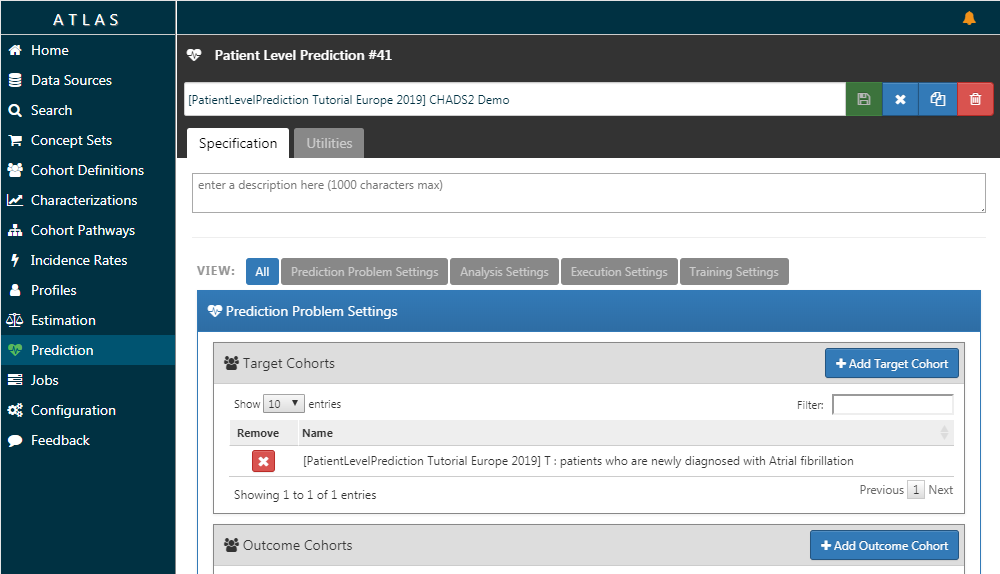
\includegraphics[width=1\linewidth]{images/PatientLevelPrediction/atlasplp1}

\begin{enumerate}
\def\labelenumi{\arabic{enumi}.}
\setcounter{enumi}{1}
\tightlist
\item
  Specify one or more analysis settings
\end{enumerate}

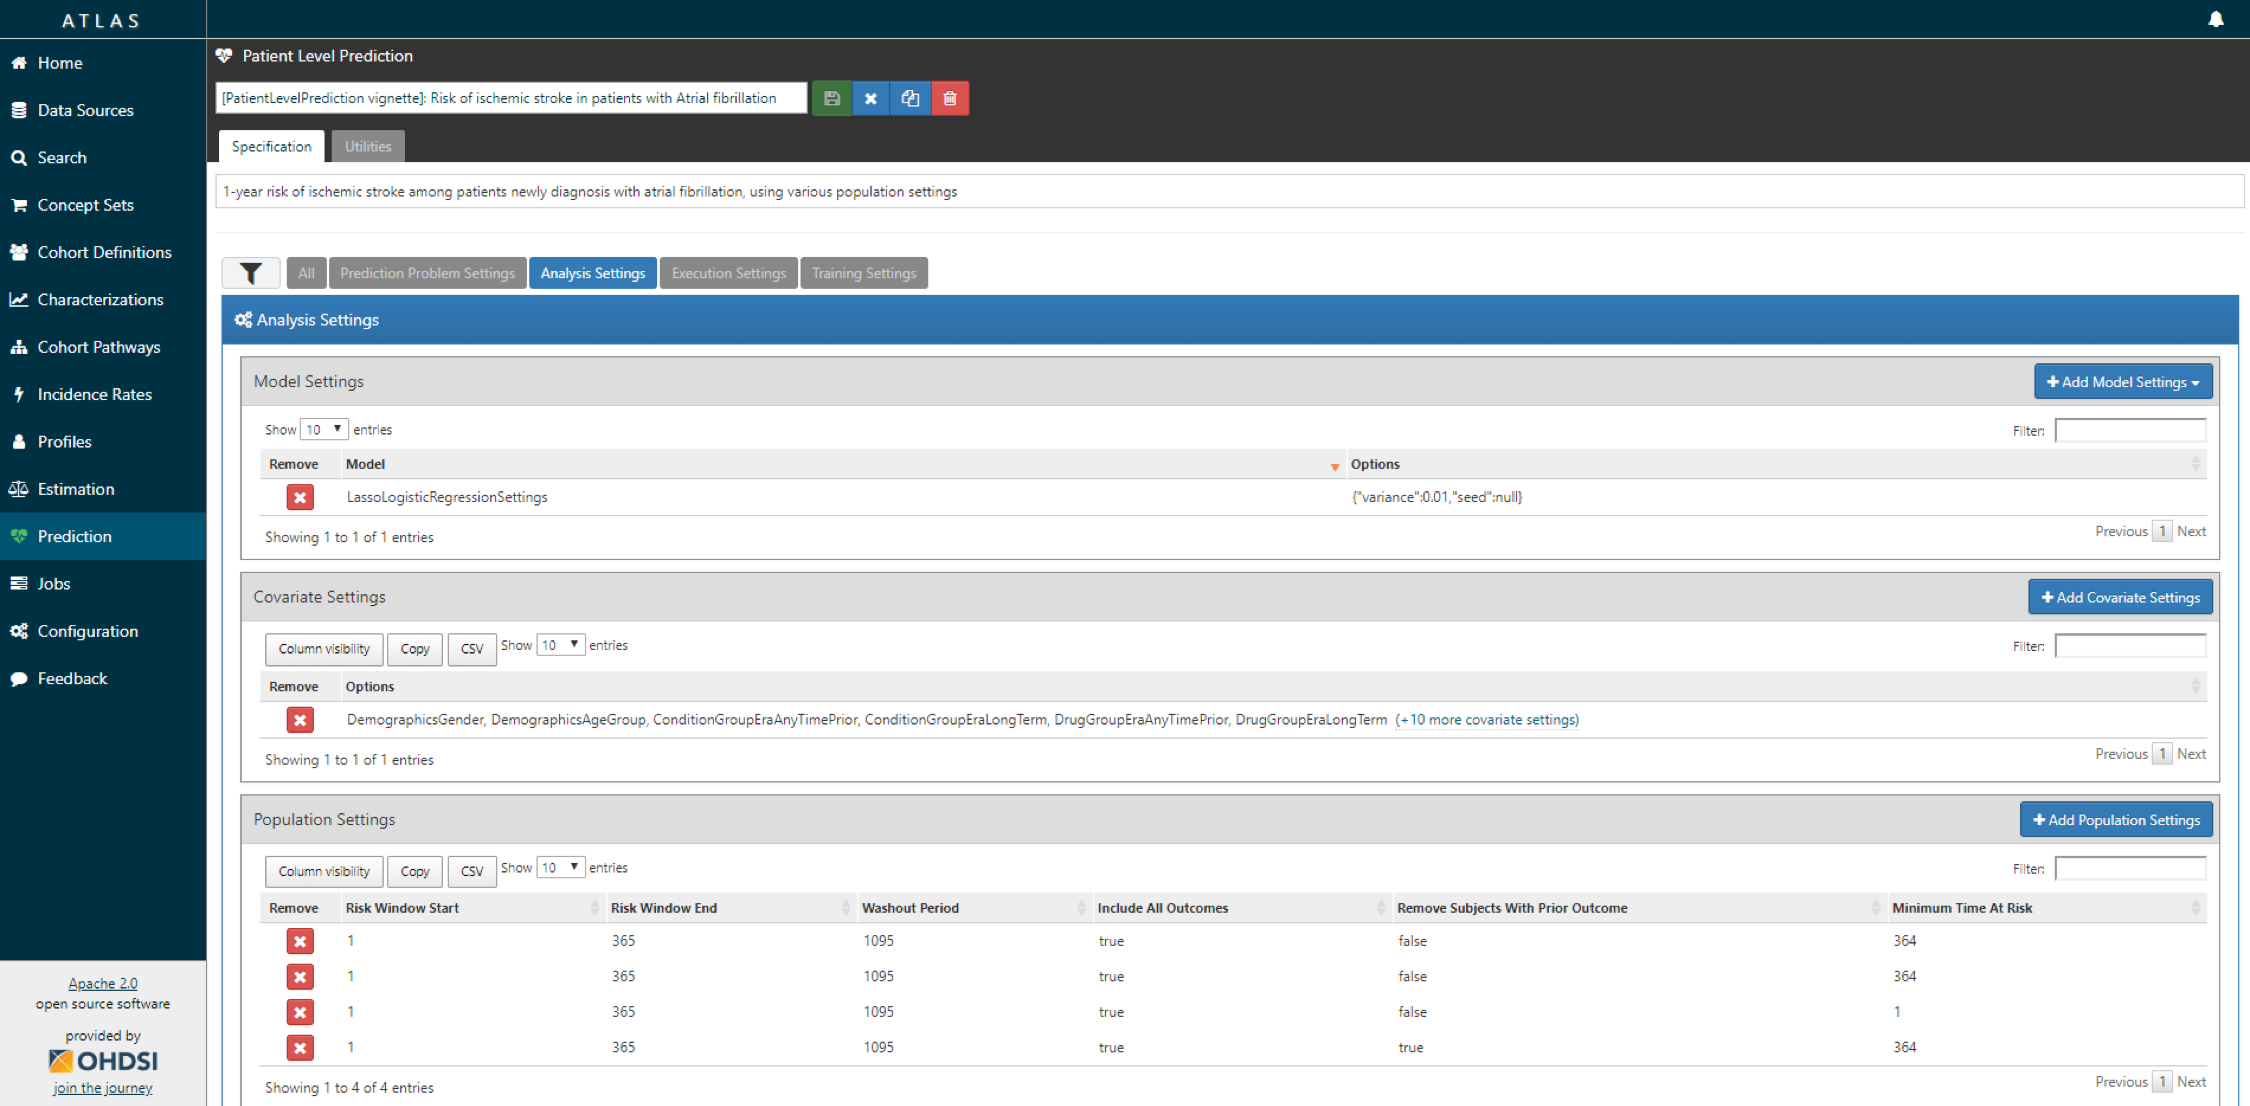
\includegraphics[width=1\linewidth]{images/PatientLevelPrediction/atlasplp2}

\newpage

\begin{enumerate}
\def\labelenumi{\arabic{enumi}.}
\setcounter{enumi}{2}
\tightlist
\item
  Specify the trainings settigns.
\end{enumerate}

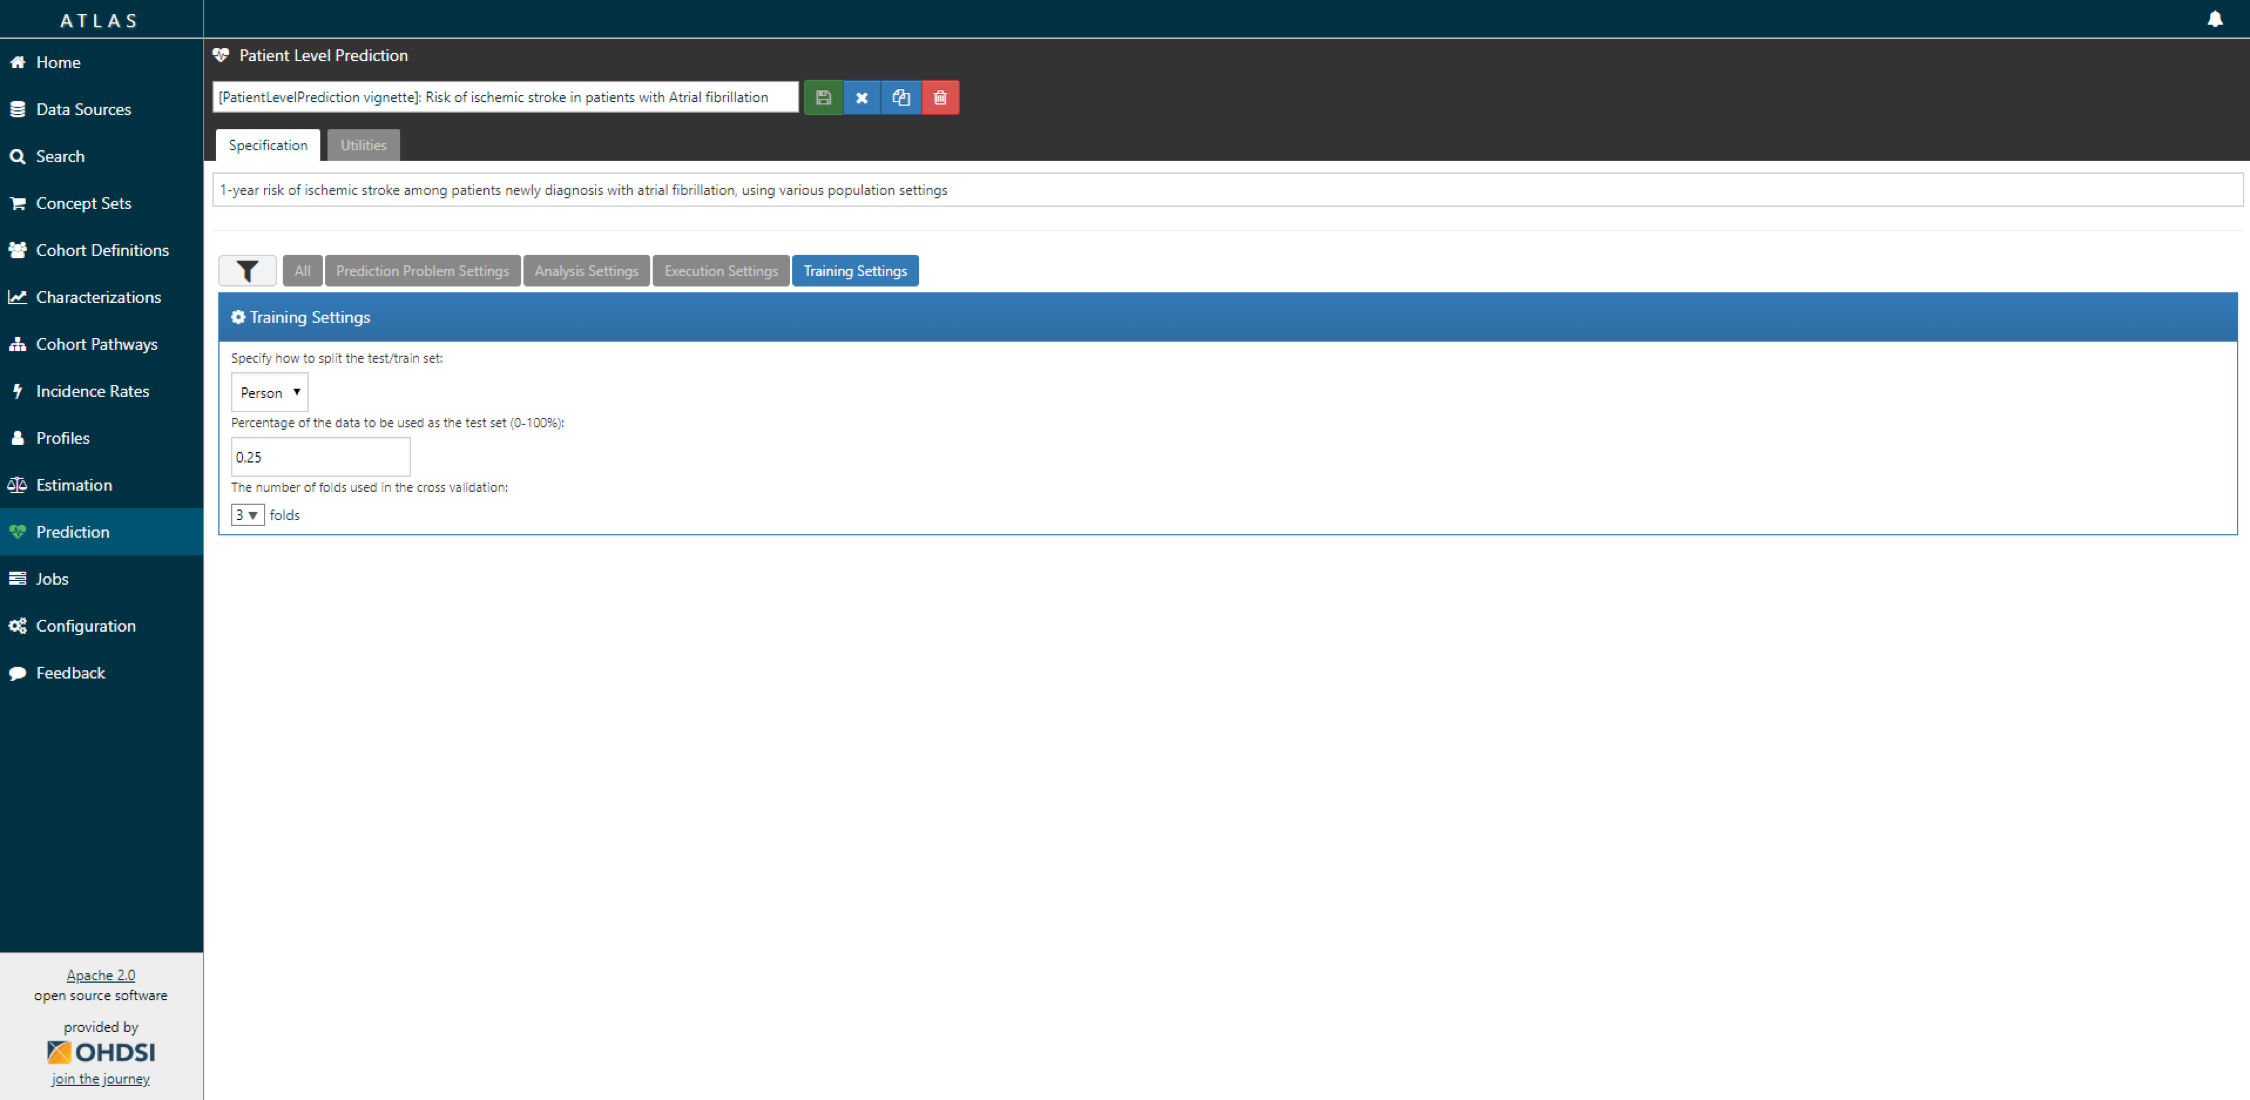
\includegraphics[width=1\linewidth]{images/PatientLevelPrediction/atlasplp3}

\begin{enumerate}
\def\labelenumi{\arabic{enumi}.}
\setcounter{enumi}{3}
\tightlist
\item
  Specify the execution settings.
\end{enumerate}

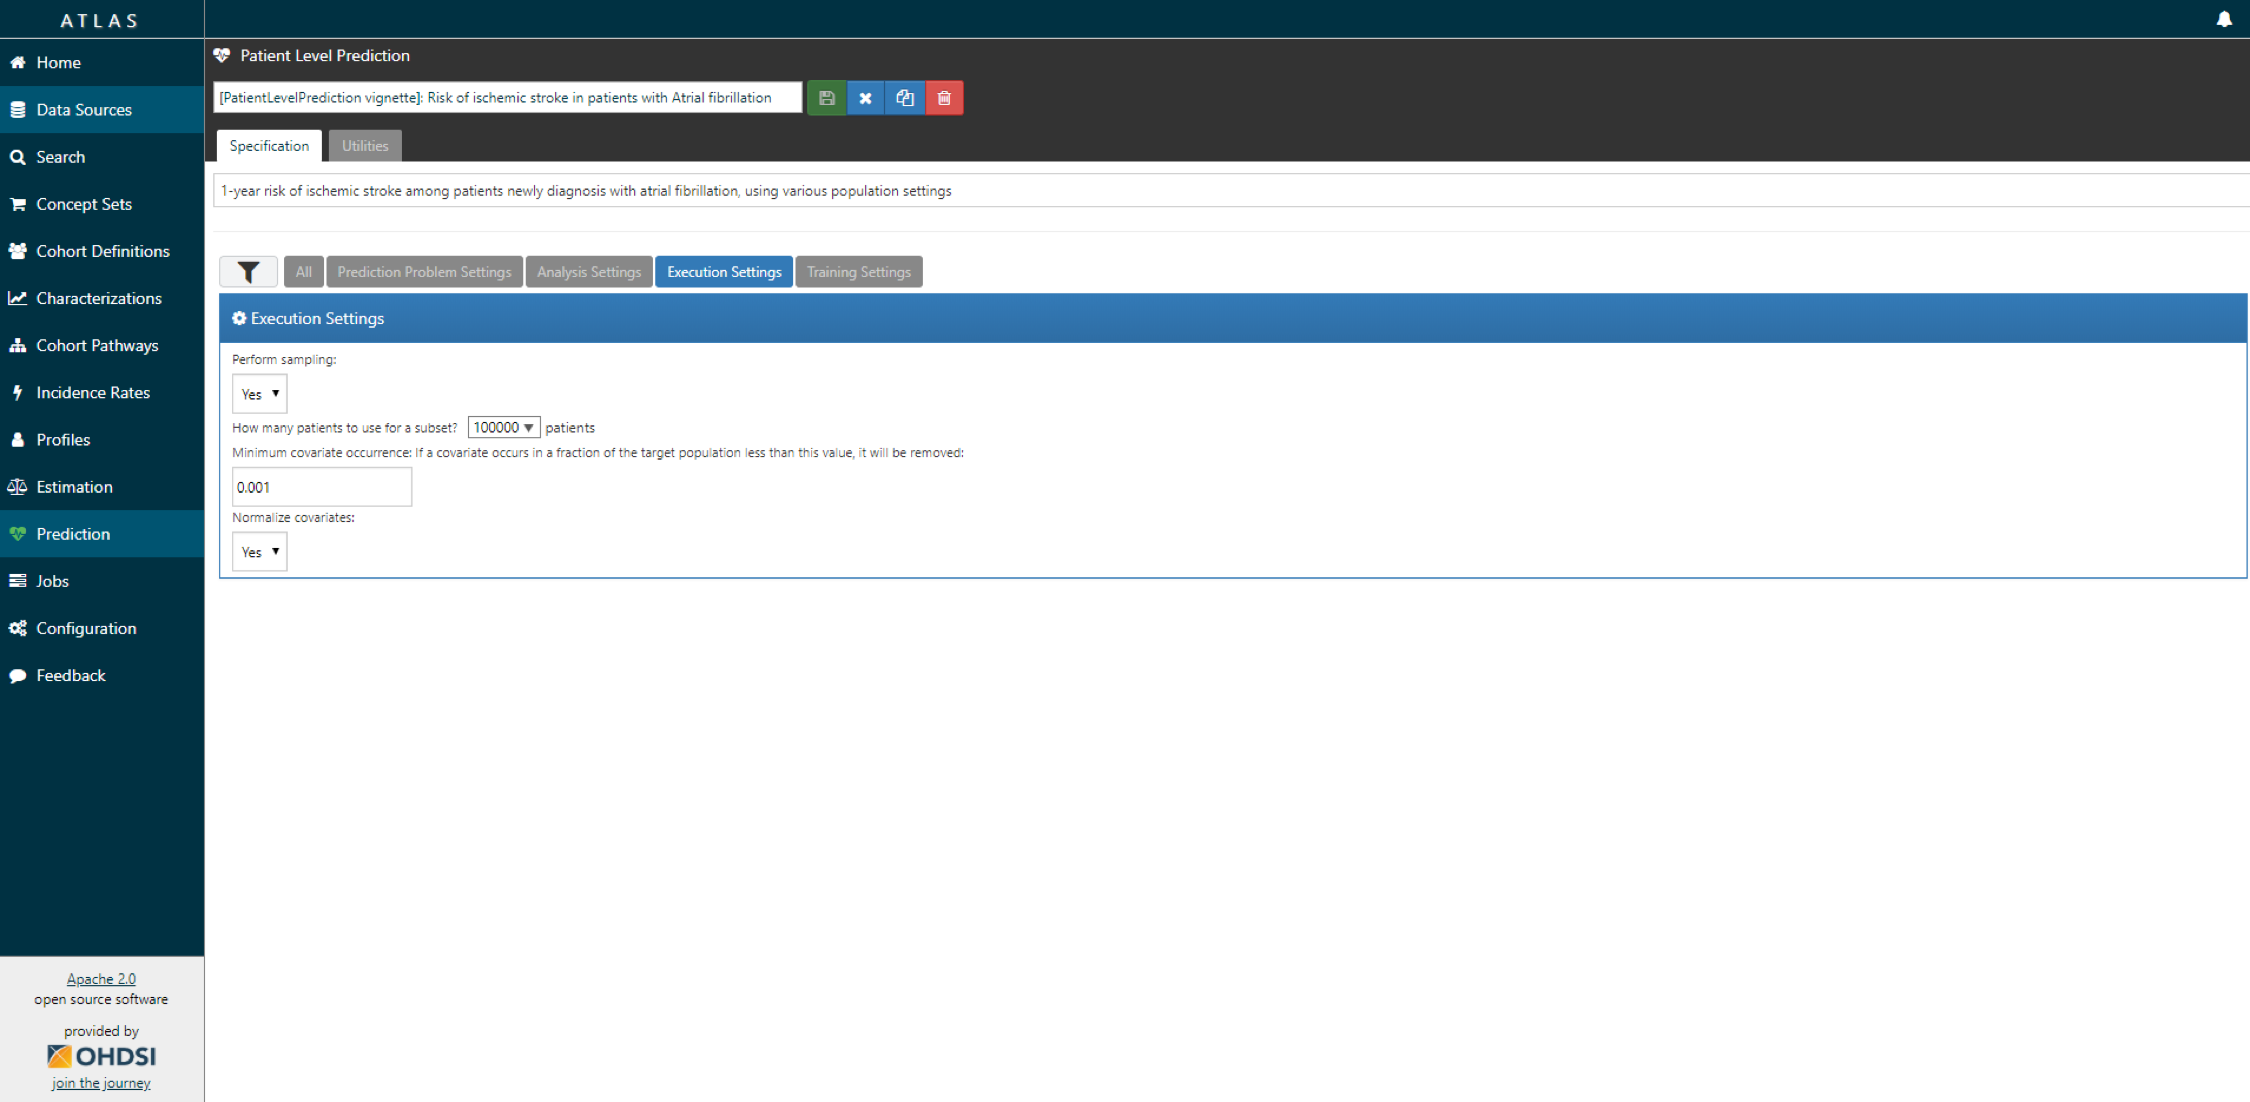
\includegraphics[width=1\linewidth]{images/PatientLevelPrediction/atlasplp4}

\newpage

ATLAS can build a R package for you that will execute the full study
against you CDM. Below the steps are explained how to do this in ATLAS.

\begin{enumerate}
\def\labelenumi{\arabic{enumi}.}
\tightlist
\item
  Under utilities you can find download. Click on the button to review
  the full study specification.
\end{enumerate}

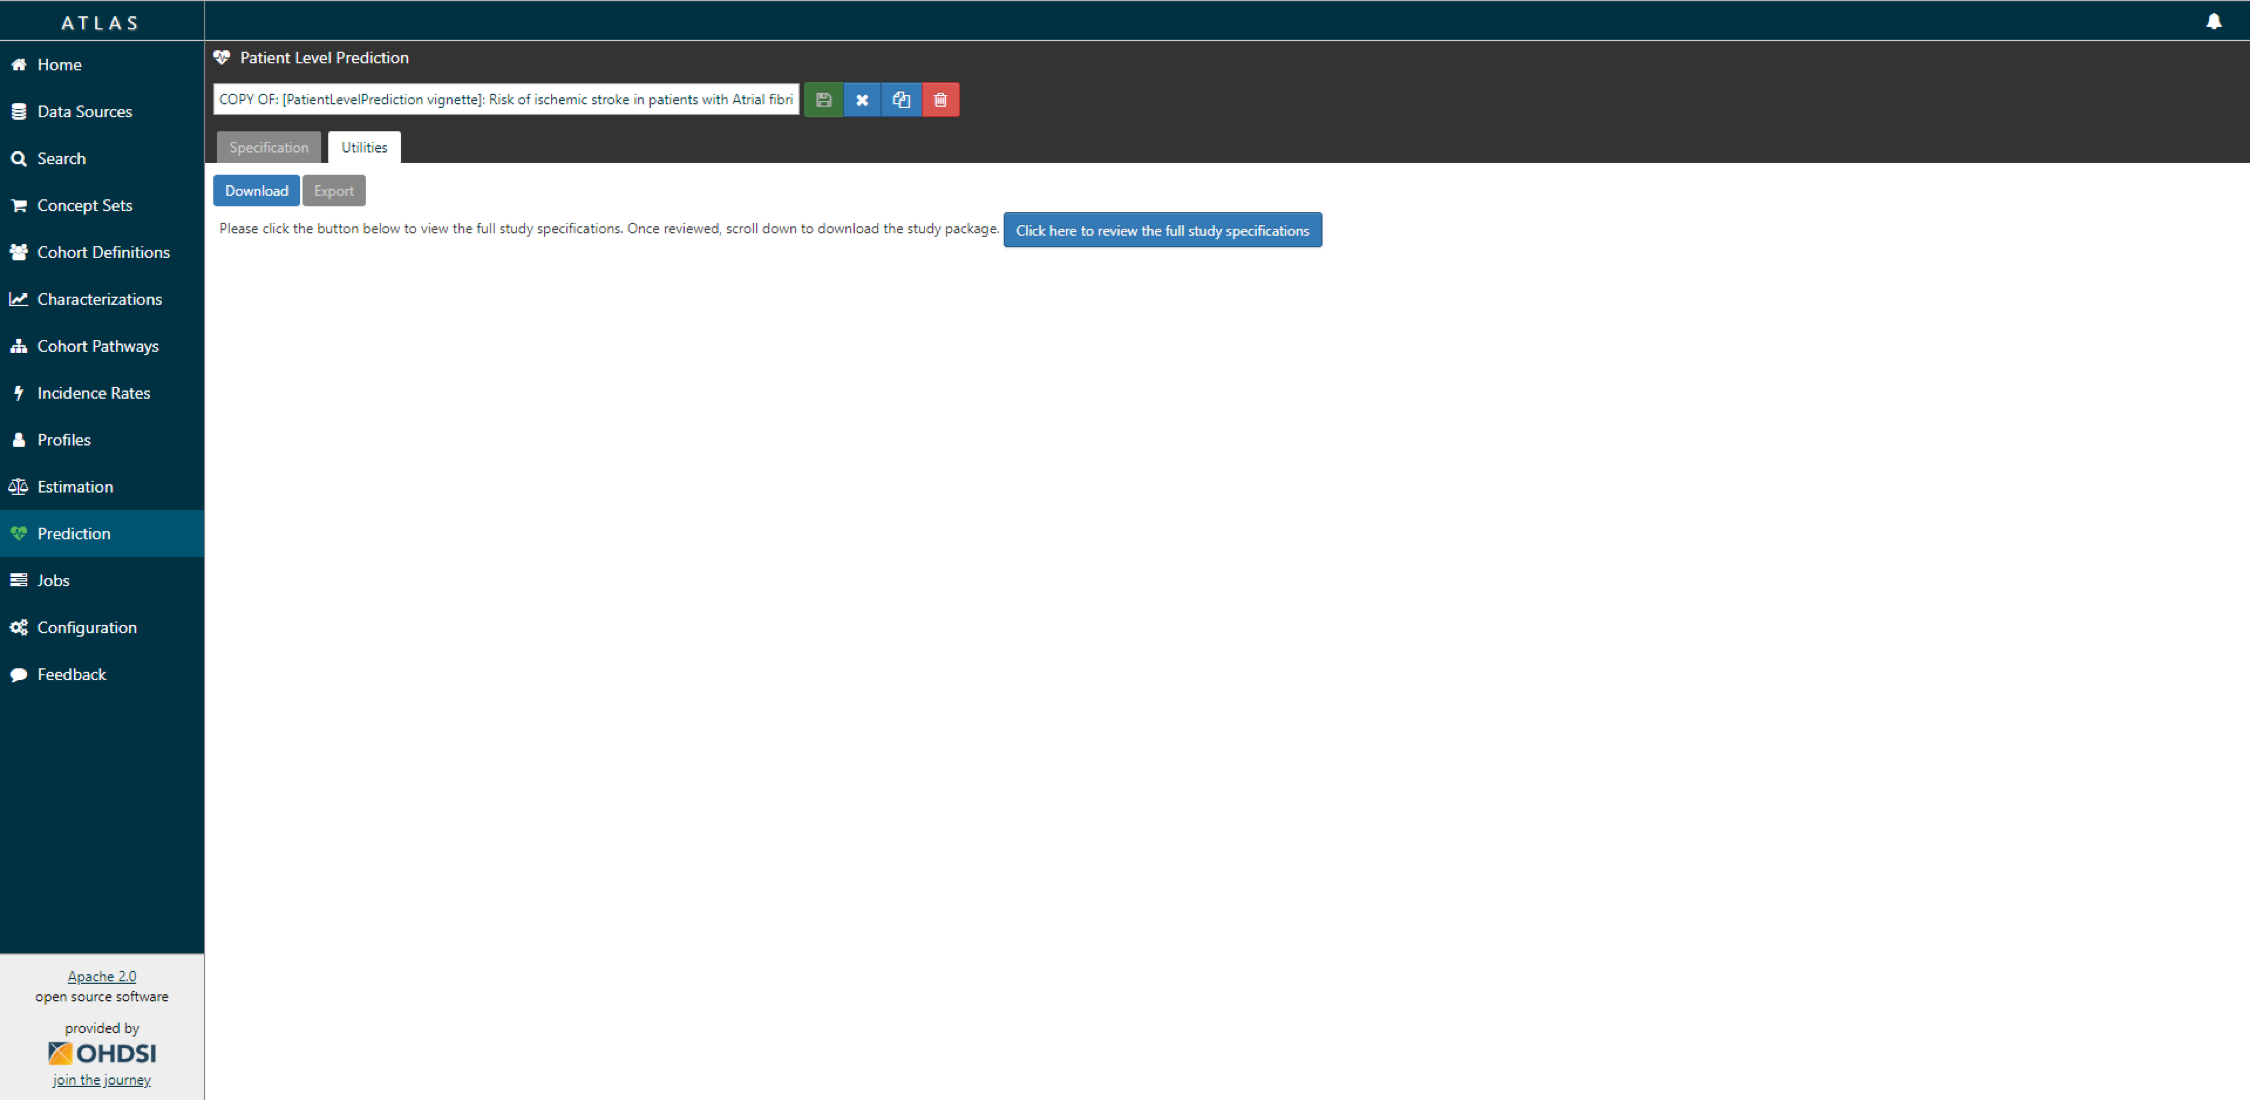
\includegraphics[width=1\linewidth]{images/PatientLevelPrediction/atlasdownload1}

\begin{enumerate}
\def\labelenumi{\arabic{enumi}.}
\setcounter{enumi}{1}
\tightlist
\item
  You now have to review that you indeed want to run all these analyses
  (cartesian product of all the settings for each T and O combination.
\end{enumerate}

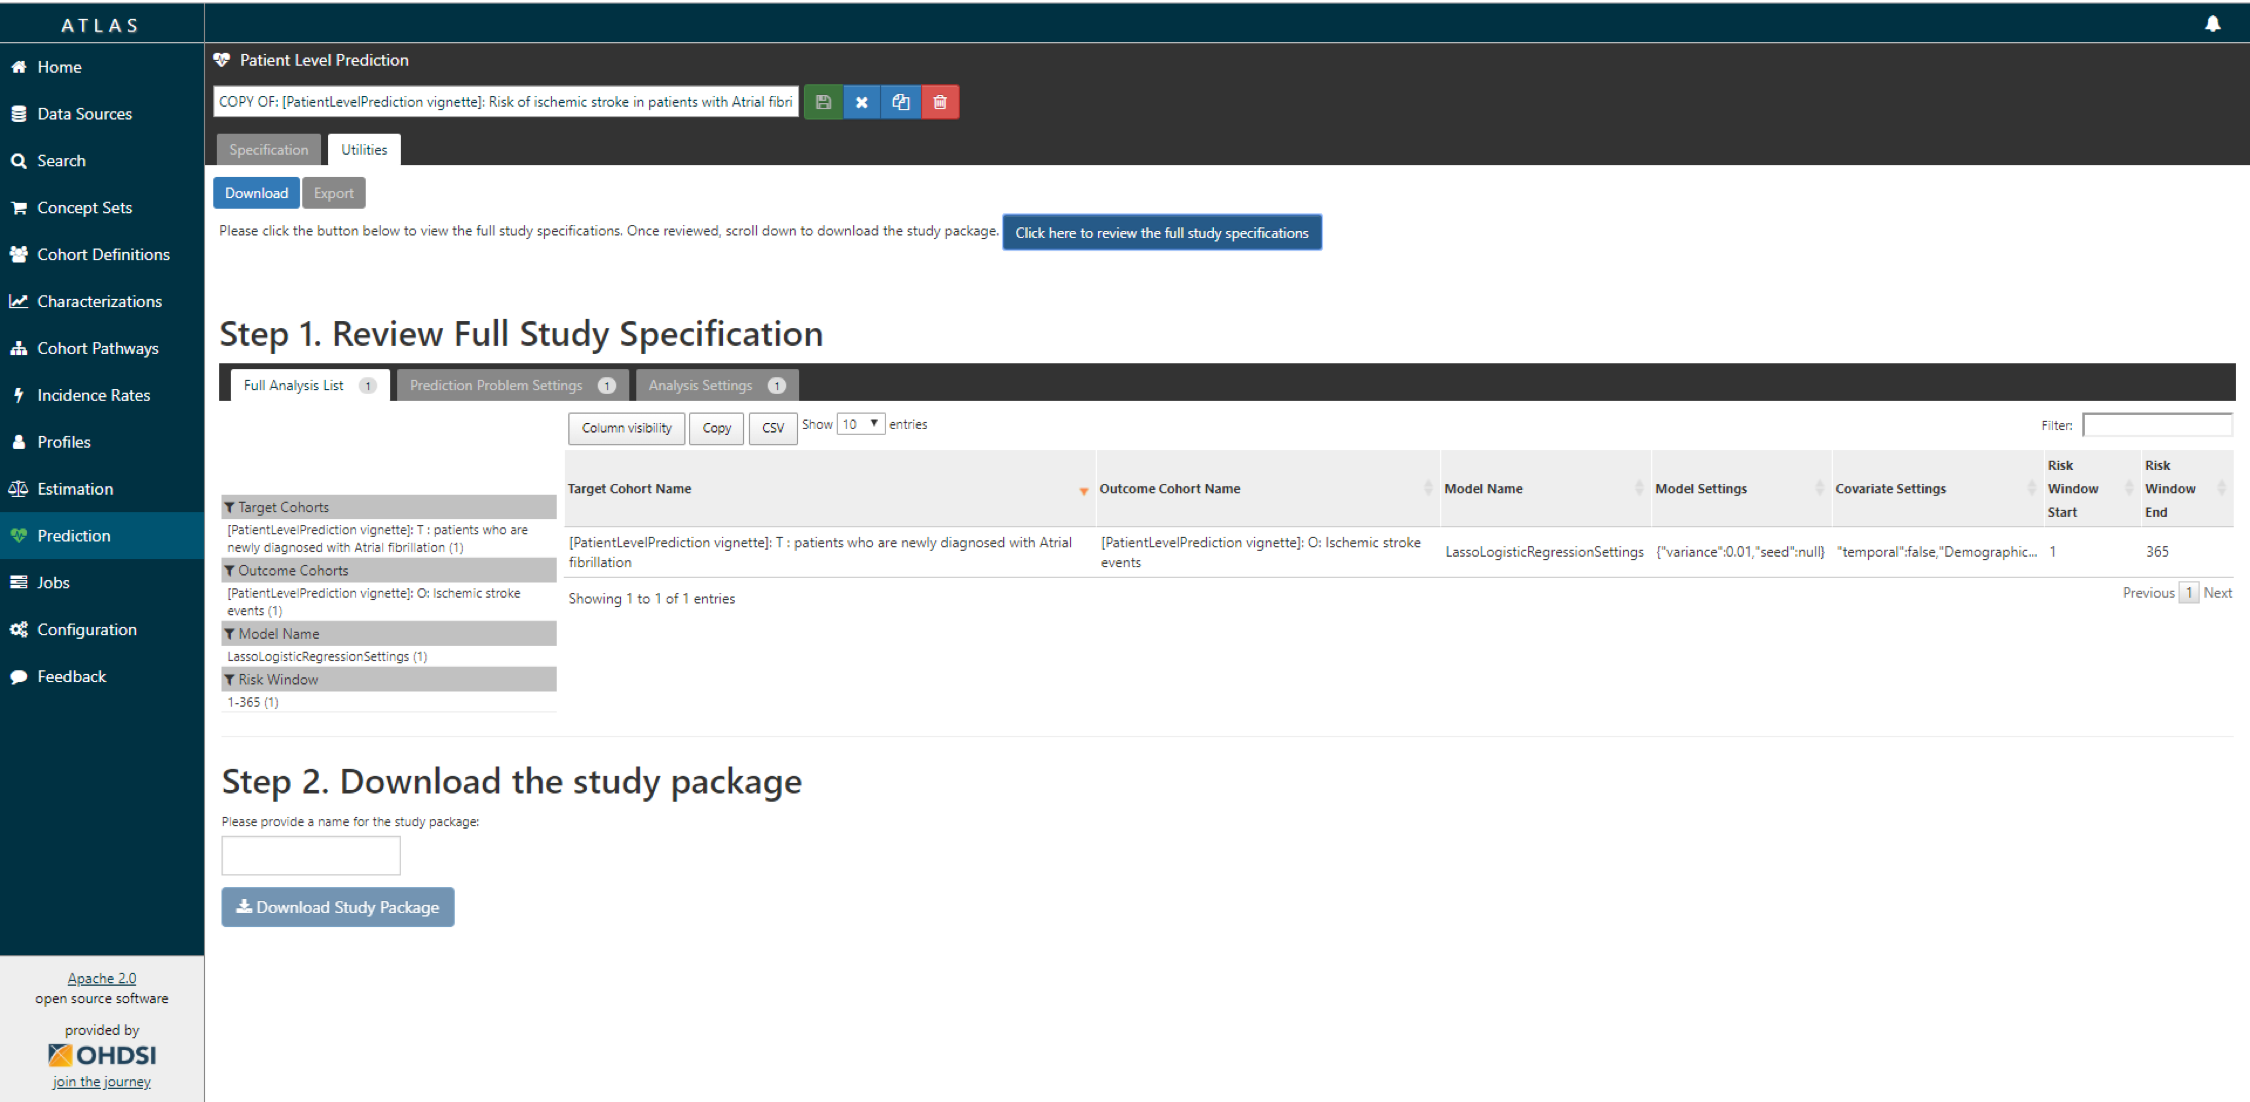
\includegraphics[width=1\linewidth]{images/PatientLevelPrediction/atlasdownload2}

\begin{enumerate}
\def\labelenumi{\arabic{enumi}.}
\setcounter{enumi}{2}
\item
  If you agree, you give the package a name, and download the package as
  a zipfile.
\item
  By opening the R package in R studio and building the package you can
  run the study using the \texttt{execute} function. Theres is also an
  example CodeToRun.R script available in the extras folder of the
  package with extra instructions.
\end{enumerate}

\section{Internal validation}\label{internal-validation}

Once we execute the study, the runPlp() function returns the trained
model and the evaluation of the model on the train/test sets.

You can interactively view the results by running:
\texttt{viewPlp(runPlp=lrResults)}. This will generate a Shiny App in
your browser in which you can view all performance measures created by
the framework as shown in the figure below.

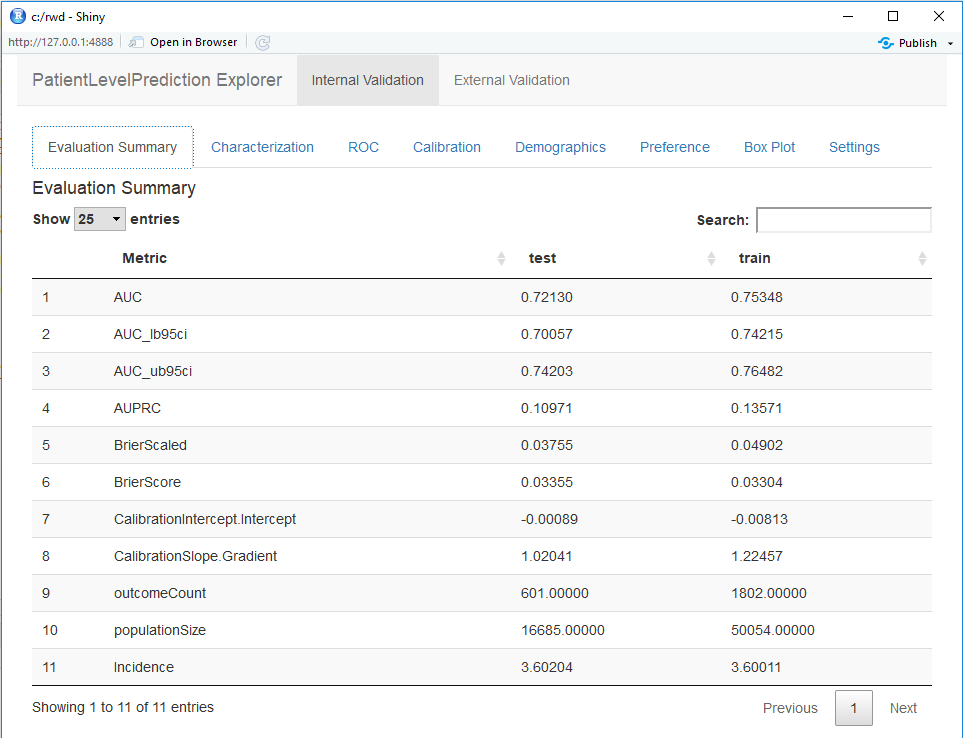
\includegraphics[width=1\linewidth]{images/PatientLevelPrediction/shinysummary}

Furthermore, many interactive plots are available in the Shiny App, for
example the ROC curve in which you can move over the plot to see the
threshold and the corresponding sensitivity and specificity values.

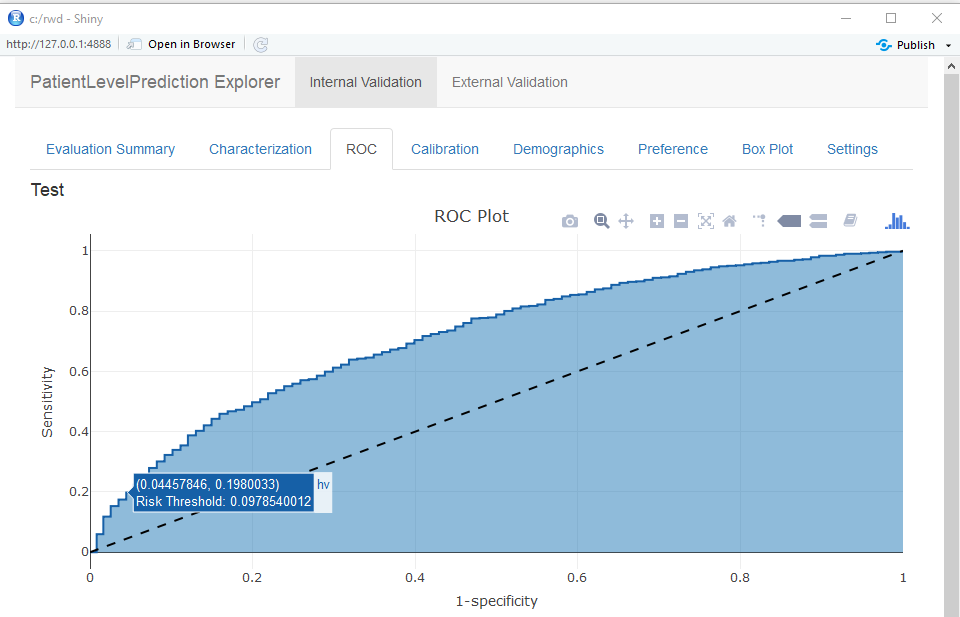
\includegraphics[width=1\linewidth]{images/PatientLevelPrediction/shinyroc}

To generate and save all the evaluation plots to a folder run the
following code:

\begin{Shaded}
\begin{Highlighting}[]
\KeywordTok{plotPlp}\NormalTok{(lrResults, }\DataTypeTok{dirPath=}\KeywordTok{getwd}\NormalTok{())}
\end{Highlighting}
\end{Shaded}

The plots are described in more detail in the next sections.

\newpage

\subsection{Discrimination}\label{discrimination}

The Receiver Operating Characteristics (ROC) plot shows the sensitivity
against 1-specificity on the test set. The plot illustrates how well the
model is able to discriminate between the people with the outcome and
those without. The dashed diagonal line is the performance of a model
that randomly assigns predictions. The higher the area under the ROC
plot the better the discrimination of the model. The plot is created by
changing the probability threshold to assign the positive class.

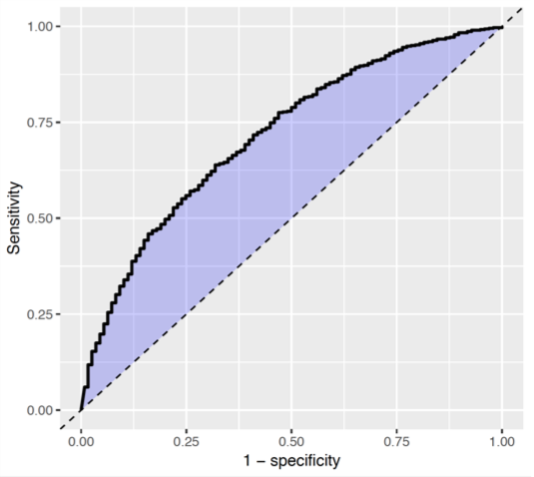
\includegraphics[width=1\linewidth]{images/PatientLevelPrediction/sparseROC}

\newpage

\subsection{Calibration}\label{calibration}

The calibration plot shows how close the predicted risk is to the
observed risk. The diagonal dashed line thus indicates a perfectly
calibrated model. The ten (or fewer) dots represent the mean predicted
values for each quantile plotted against the observed fraction of people
in that quantile who had the outcome (observed fraction). The straight
black line is the linear regression using these 10 plotted quantile mean
predicted vs observed fraction points. The straight vertical lines
represented the 95\% lower and upper confidence intervals of the slope
of the fitted line.

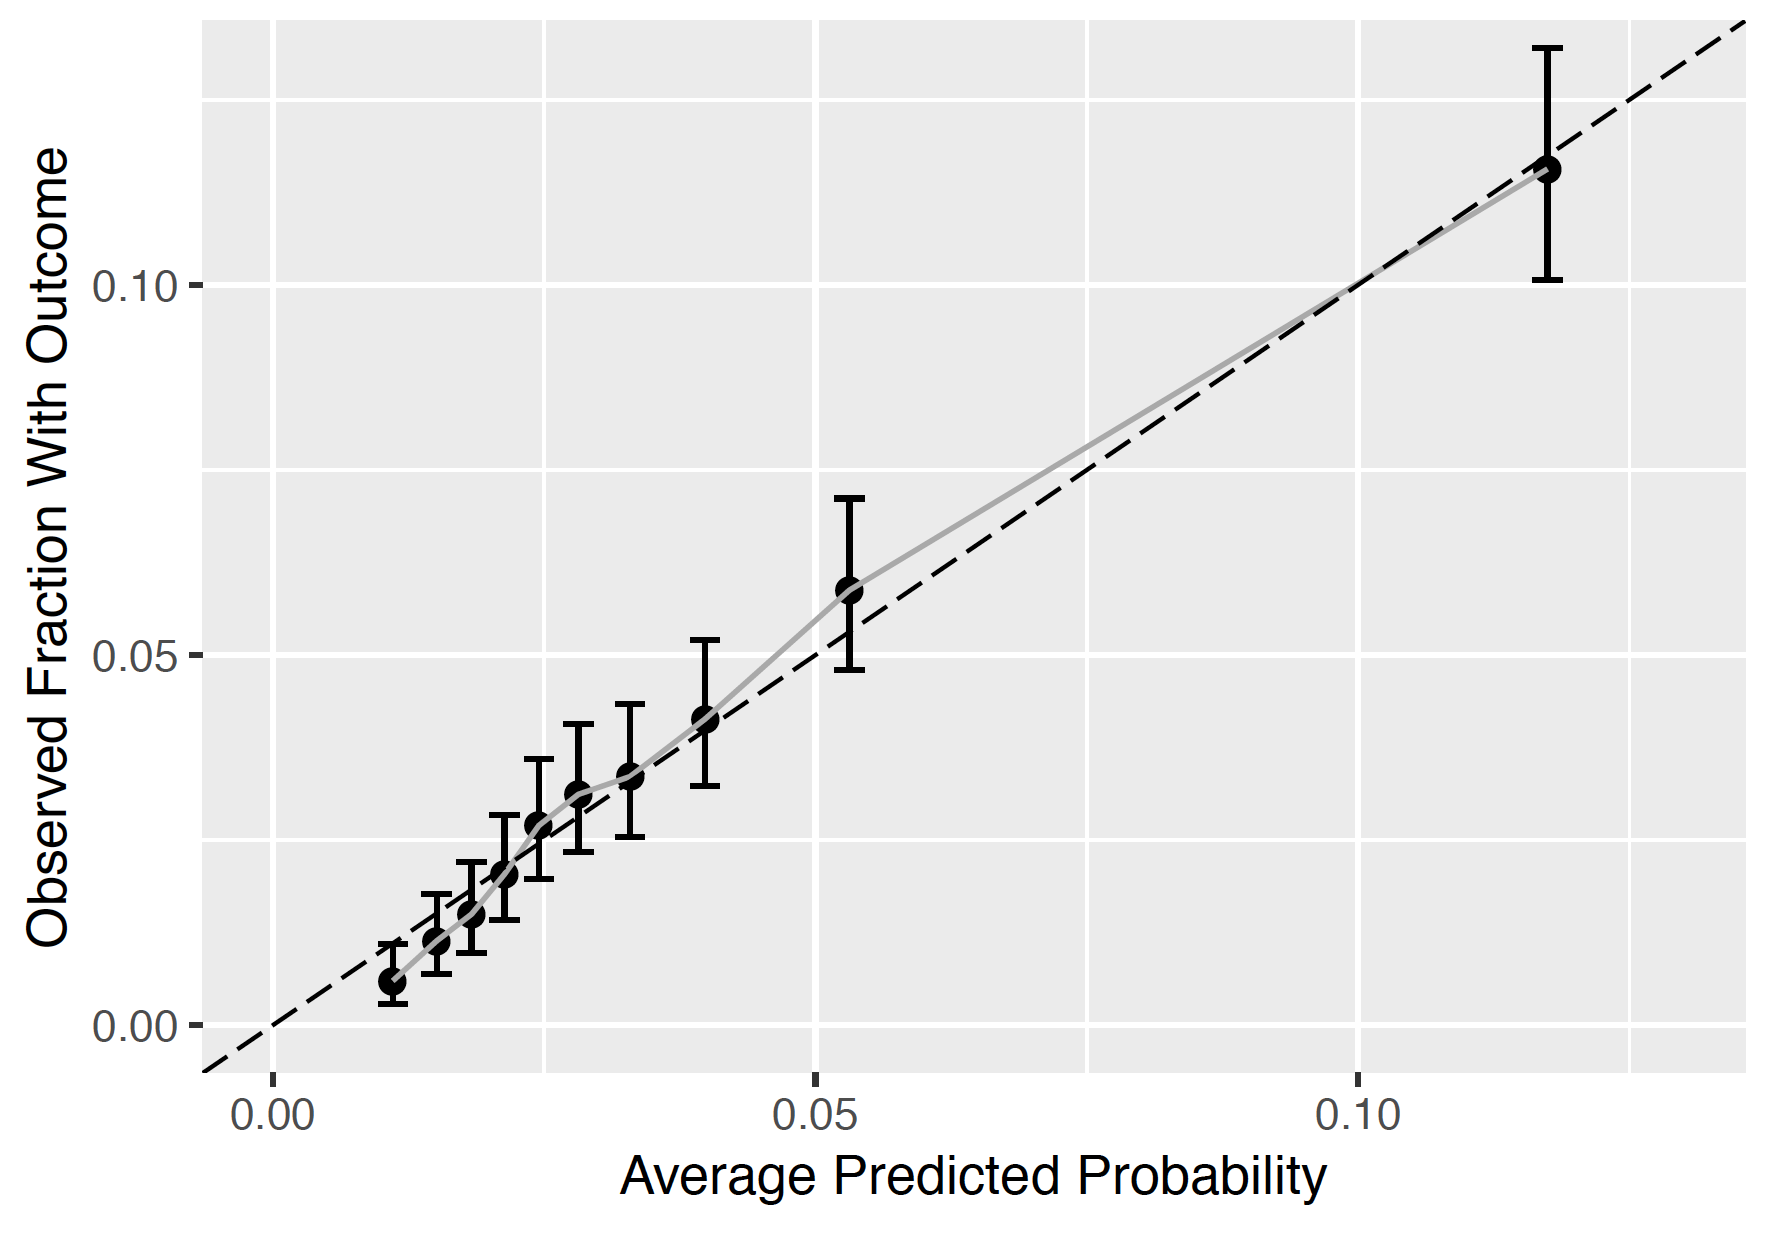
\includegraphics[width=1\linewidth]{images/PatientLevelPrediction/sparseCalibration}

\newpage

\subsection{Smooth Calibration}\label{smooth-calibration}

Similar to the traditional calibration shown above the Smooth
Calibration plot shows the relationship between predicted and observed
risk. the major difference is that the smooth fit allows for a more fine
grained examination of this. Whereas the traditional plot will be
heavily influenced by the areas with the highest density of data the
smooth plot will provide the same information for this region as well as
a more accurate interpretation of areas with lower density. the plot
also contains information on the distribution of the outcomes relative
to predicted risk.

However, the increased information gain comes at a computational cost.
It is recommended to use the traditional plot for examination and then
to produce the smooth plot for final versions. To create the smooth
calibarion plot you have to run the follow command:

\begin{Shaded}
\begin{Highlighting}[]
\KeywordTok{plotSmoothCalibration}\NormalTok{(lrResults)}
\end{Highlighting}
\end{Shaded}

See the help function for more information, on how to set the smoothing
method etc.

The example below is from another study that better demonstrates the
impact of using a smooth calibration plot. The default line fit would
not highlight the miss-calibration at the lower predicted probability
levels that well.

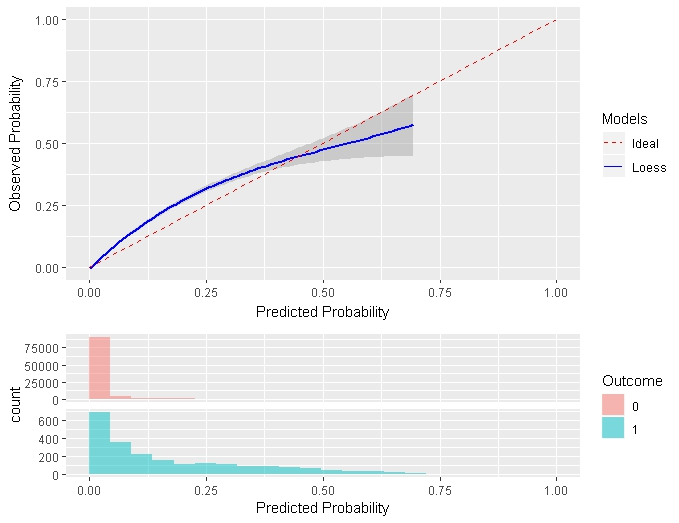
\includegraphics[width=1\linewidth]{images/PatientLevelPrediction/smoothCalibration}

\newpage

\subsection{Preference distribution}\label{preference-distribution}

The preference distribution plots are the preference score distributions
corresponding to i) people in the test set with the outcome (red) and
ii) people in the test set without the outcome (blue).

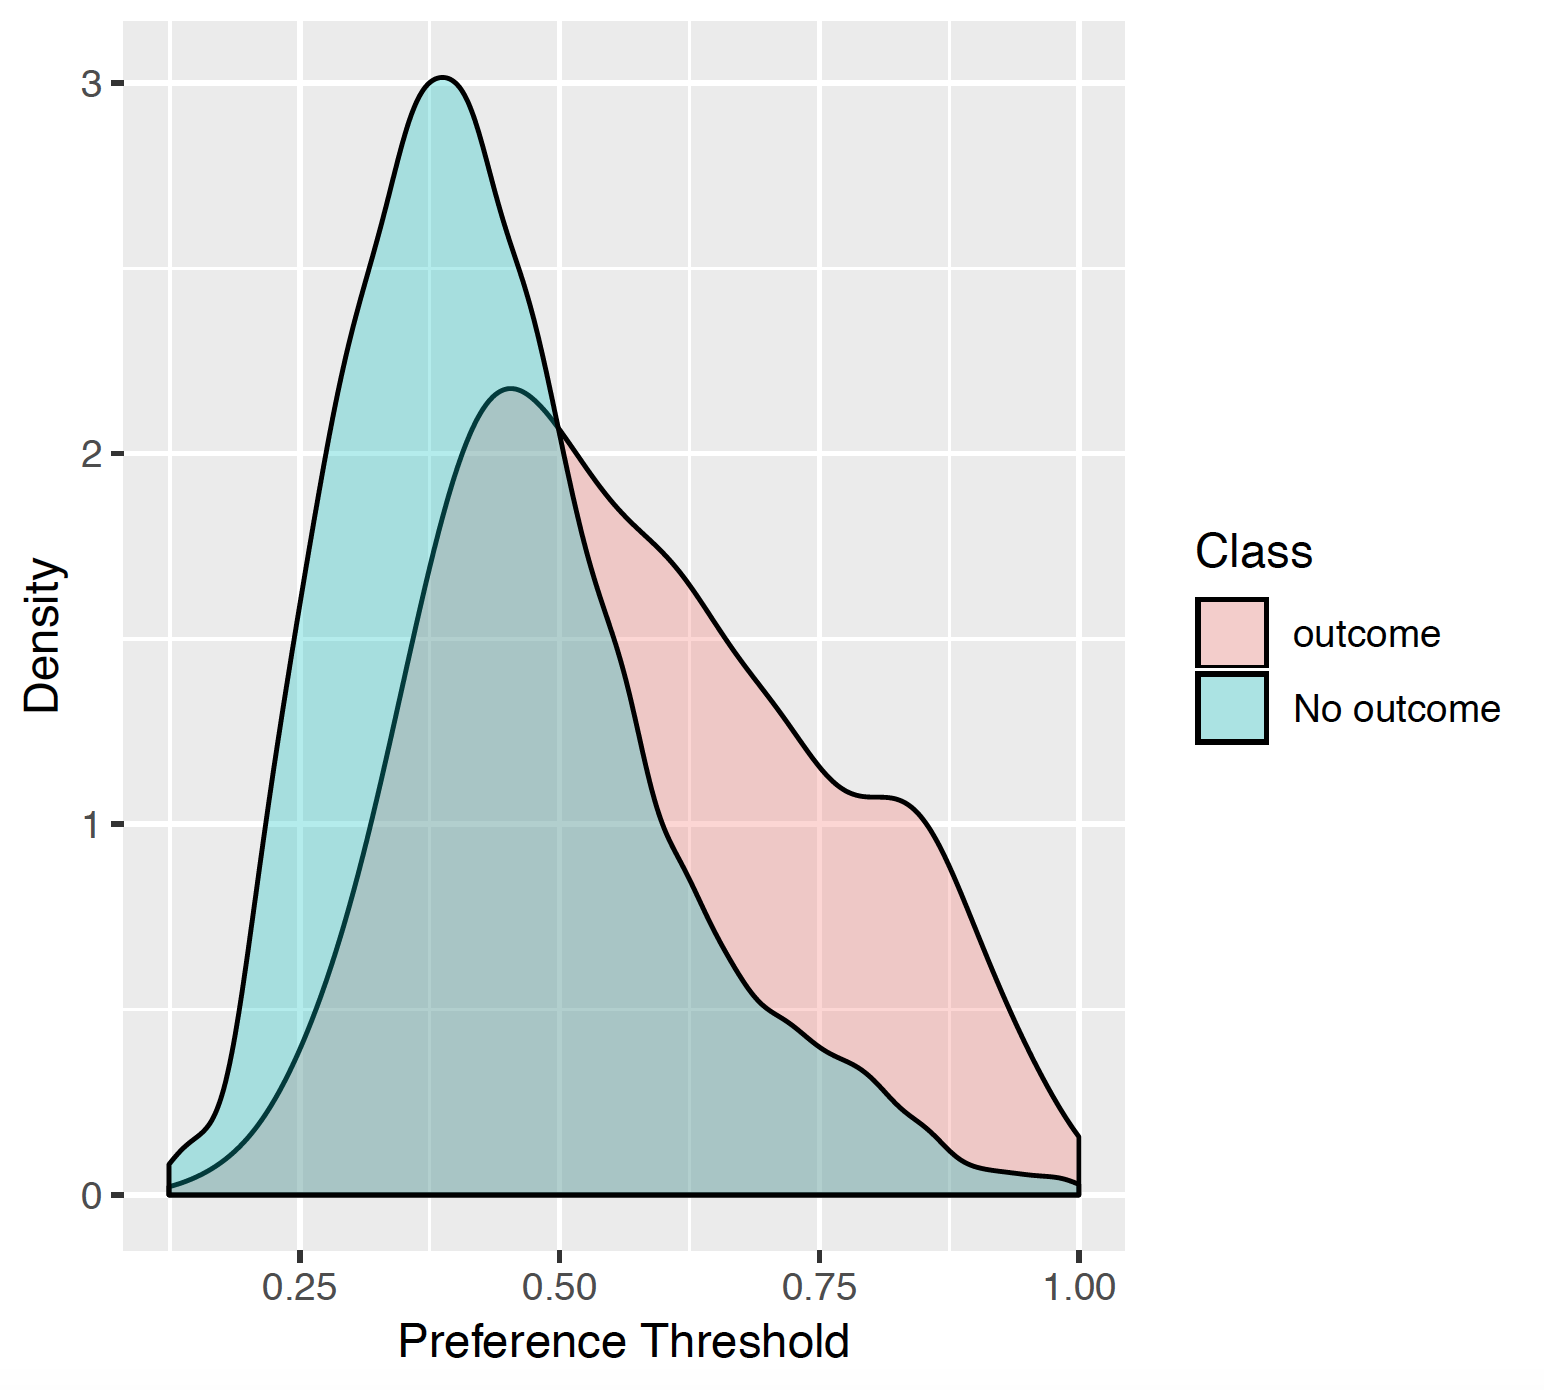
\includegraphics[width=1\linewidth]{images/PatientLevelPrediction/preferencePDF}

\newpage

\subsection{Predicted probability
distribution}\label{predicted-probability-distribution}

The prediction distribution box plots are for the predicted risks of the
people in the test set with the outcome (class 1: blue) and without the
outcome (class 0: red).

The box plots in the Figure show that the predicted probability of the
outcome is indeed higher for those with the outcome but there is also
overlap between the two distribution which lead to an imperfect
discrimination.

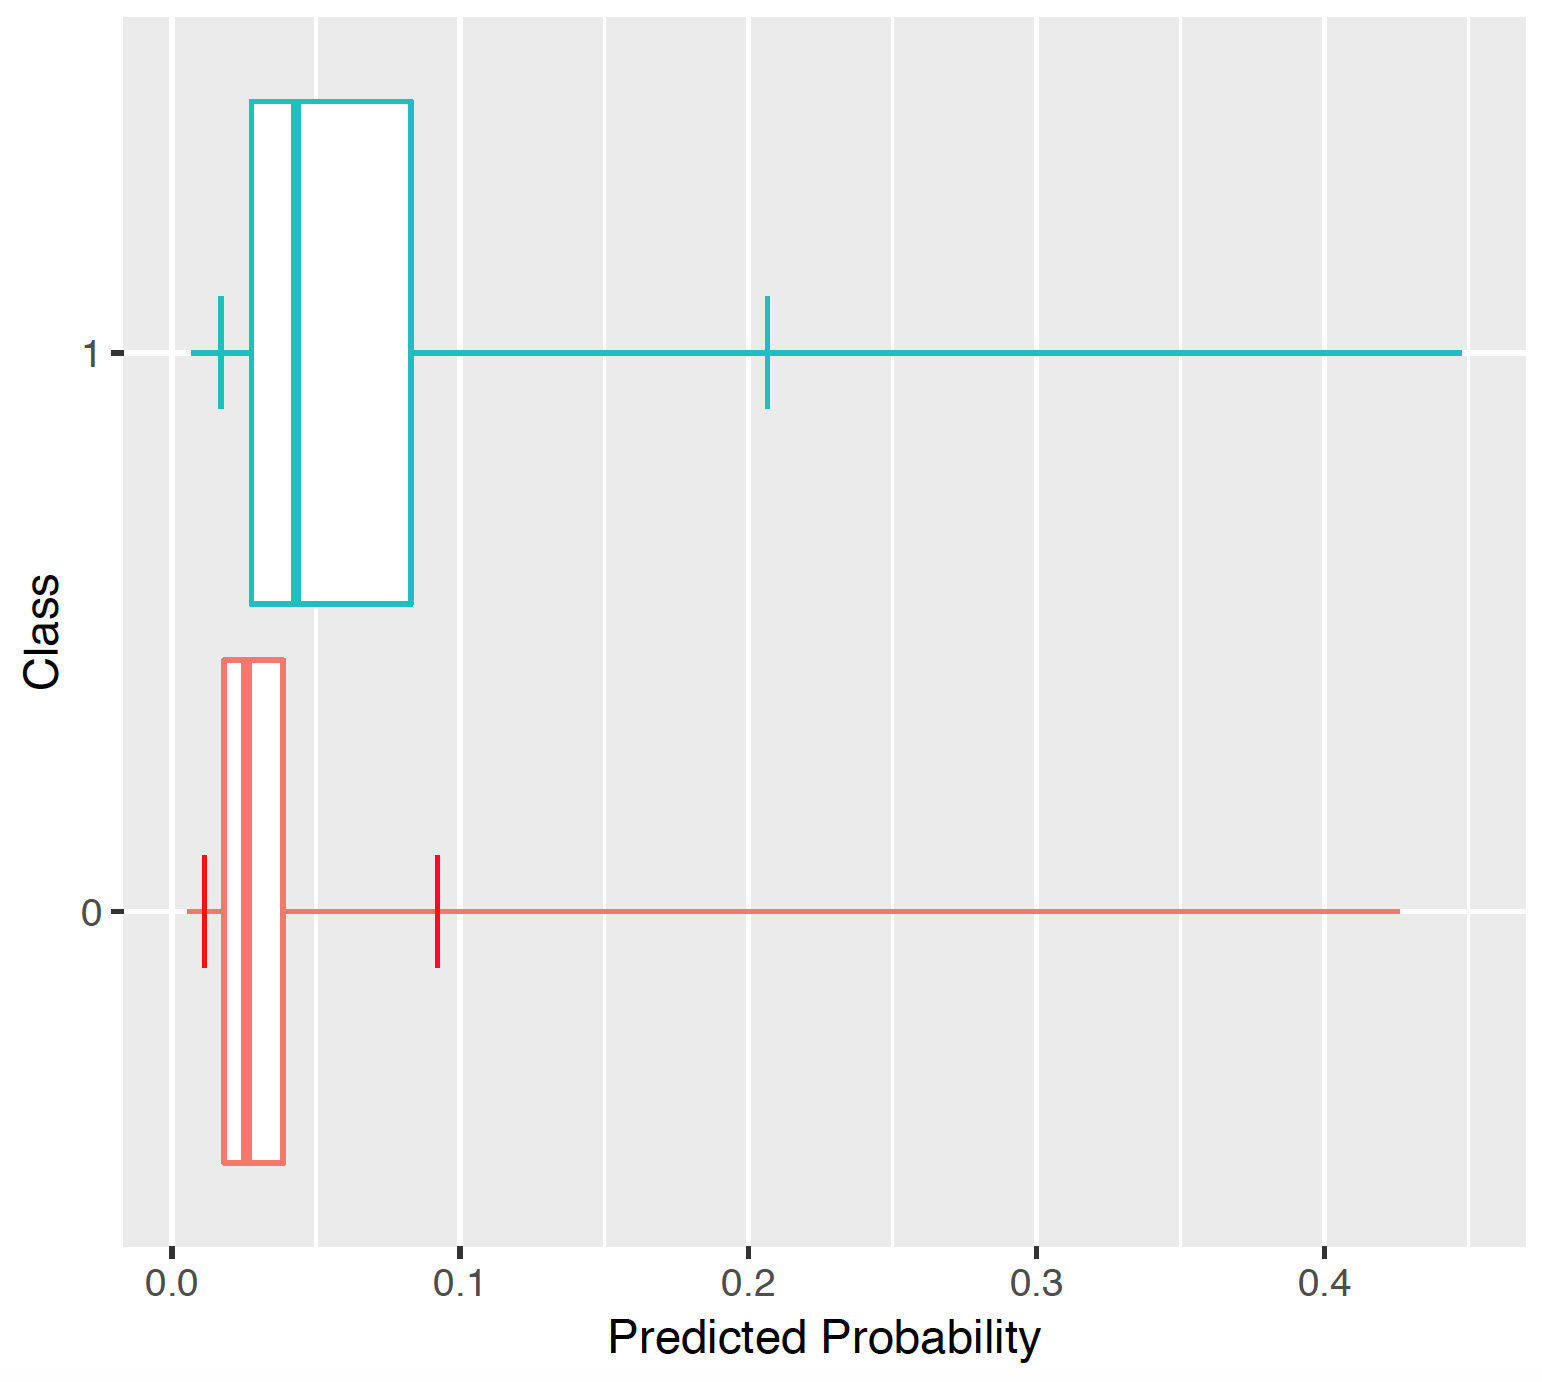
\includegraphics[width=1\linewidth]{images/PatientLevelPrediction/predictionDistribution}

\newpage

\subsection{Test-Train similarity}\label{test-train-similarity}

The test-train similarity is assessed by plotting the mean covariate
values in the train set against those in the test set for people with
and without the outcome.

The results for our example of look very promising since the mean values
of the covariates are on the diagonal.

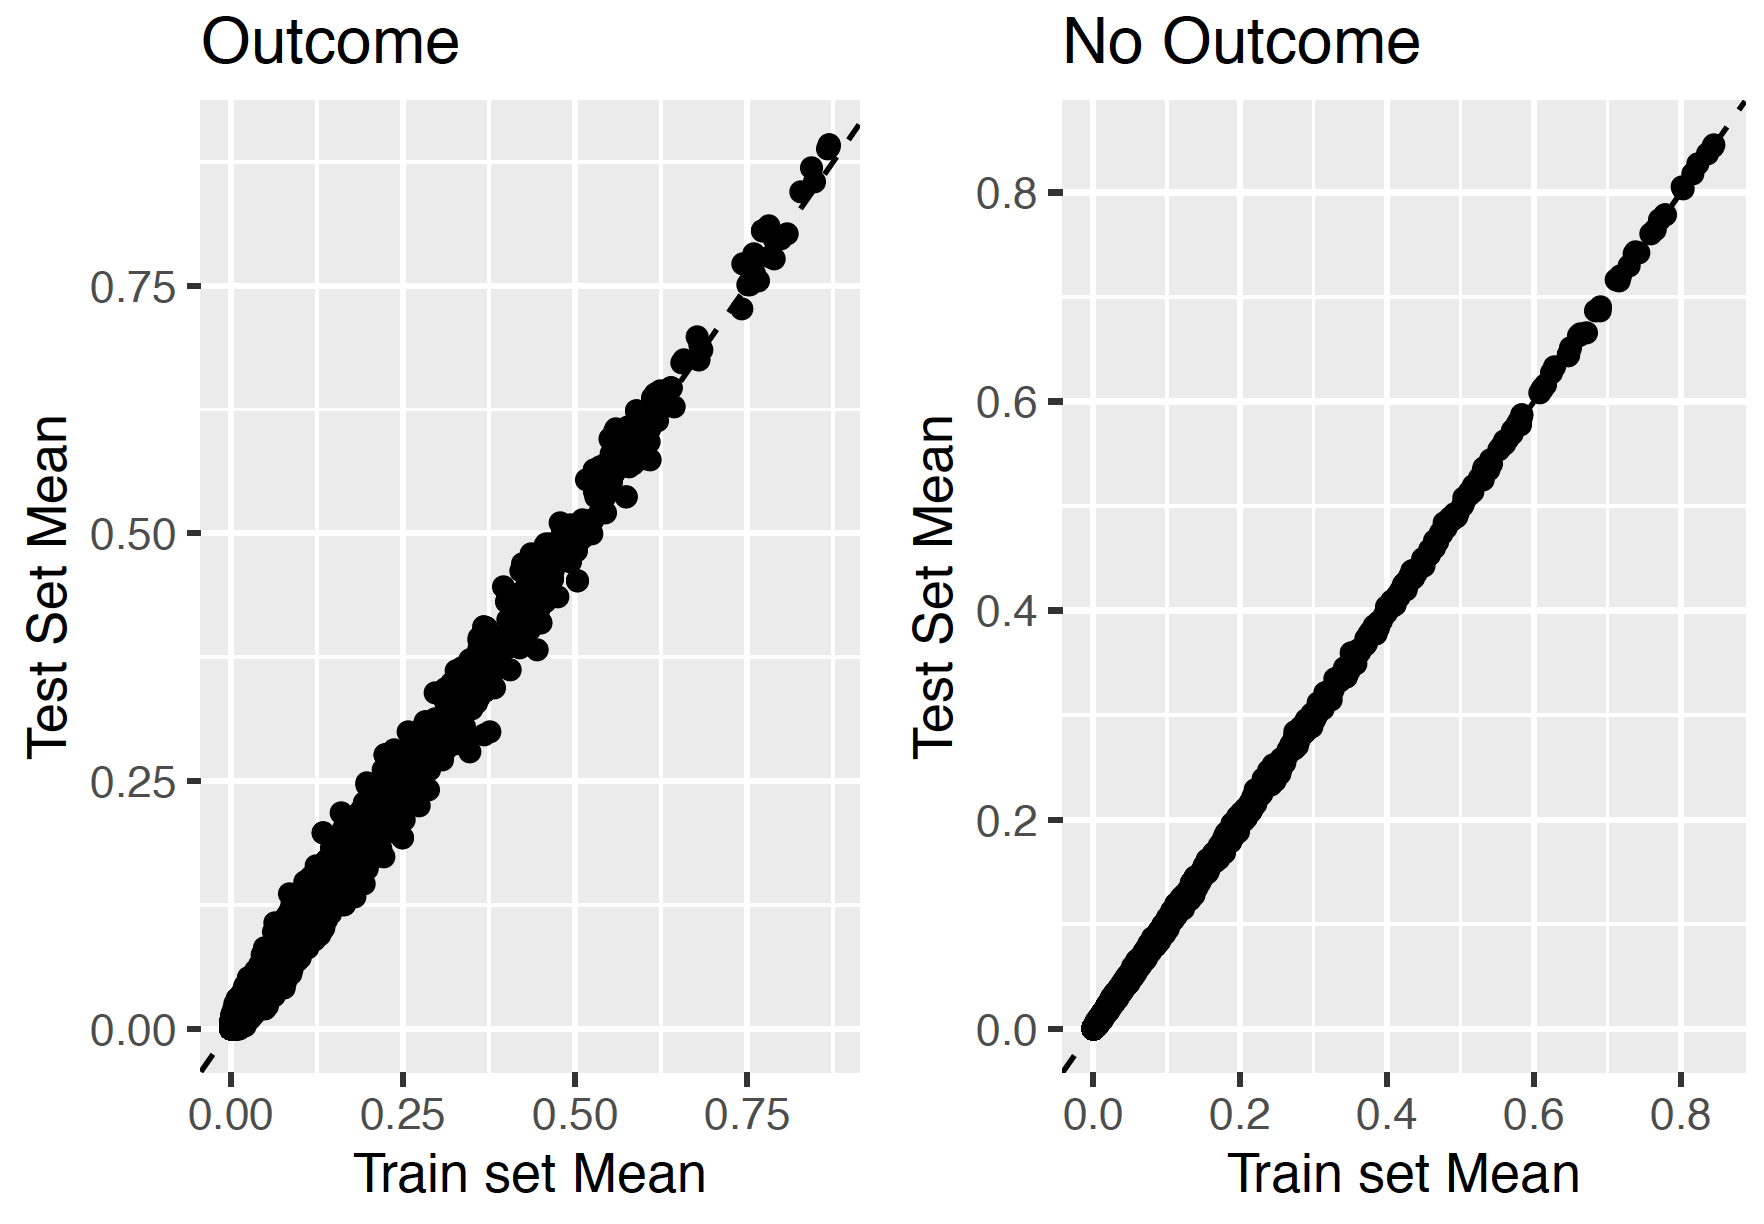
\includegraphics[width=1\linewidth]{images/PatientLevelPrediction/generalizability}

\newpage

\subsection{Variable scatter plot}\label{variable-scatter-plot}

The variable scatter plot shows the mean covariate value for the people
with the outcome against the mean covariate value for the people without
the outcome. The color of the dots corresponds to the inclusion (green)
or exclusion in the model (blue), respectively. It is highly recommended
to use the Shiny App since this allows you to hoover over a covariate to
show more details (name, value etc).

The plot shows that the mean of most of the covariates is higher for
subjects with the outcome compared to those without.

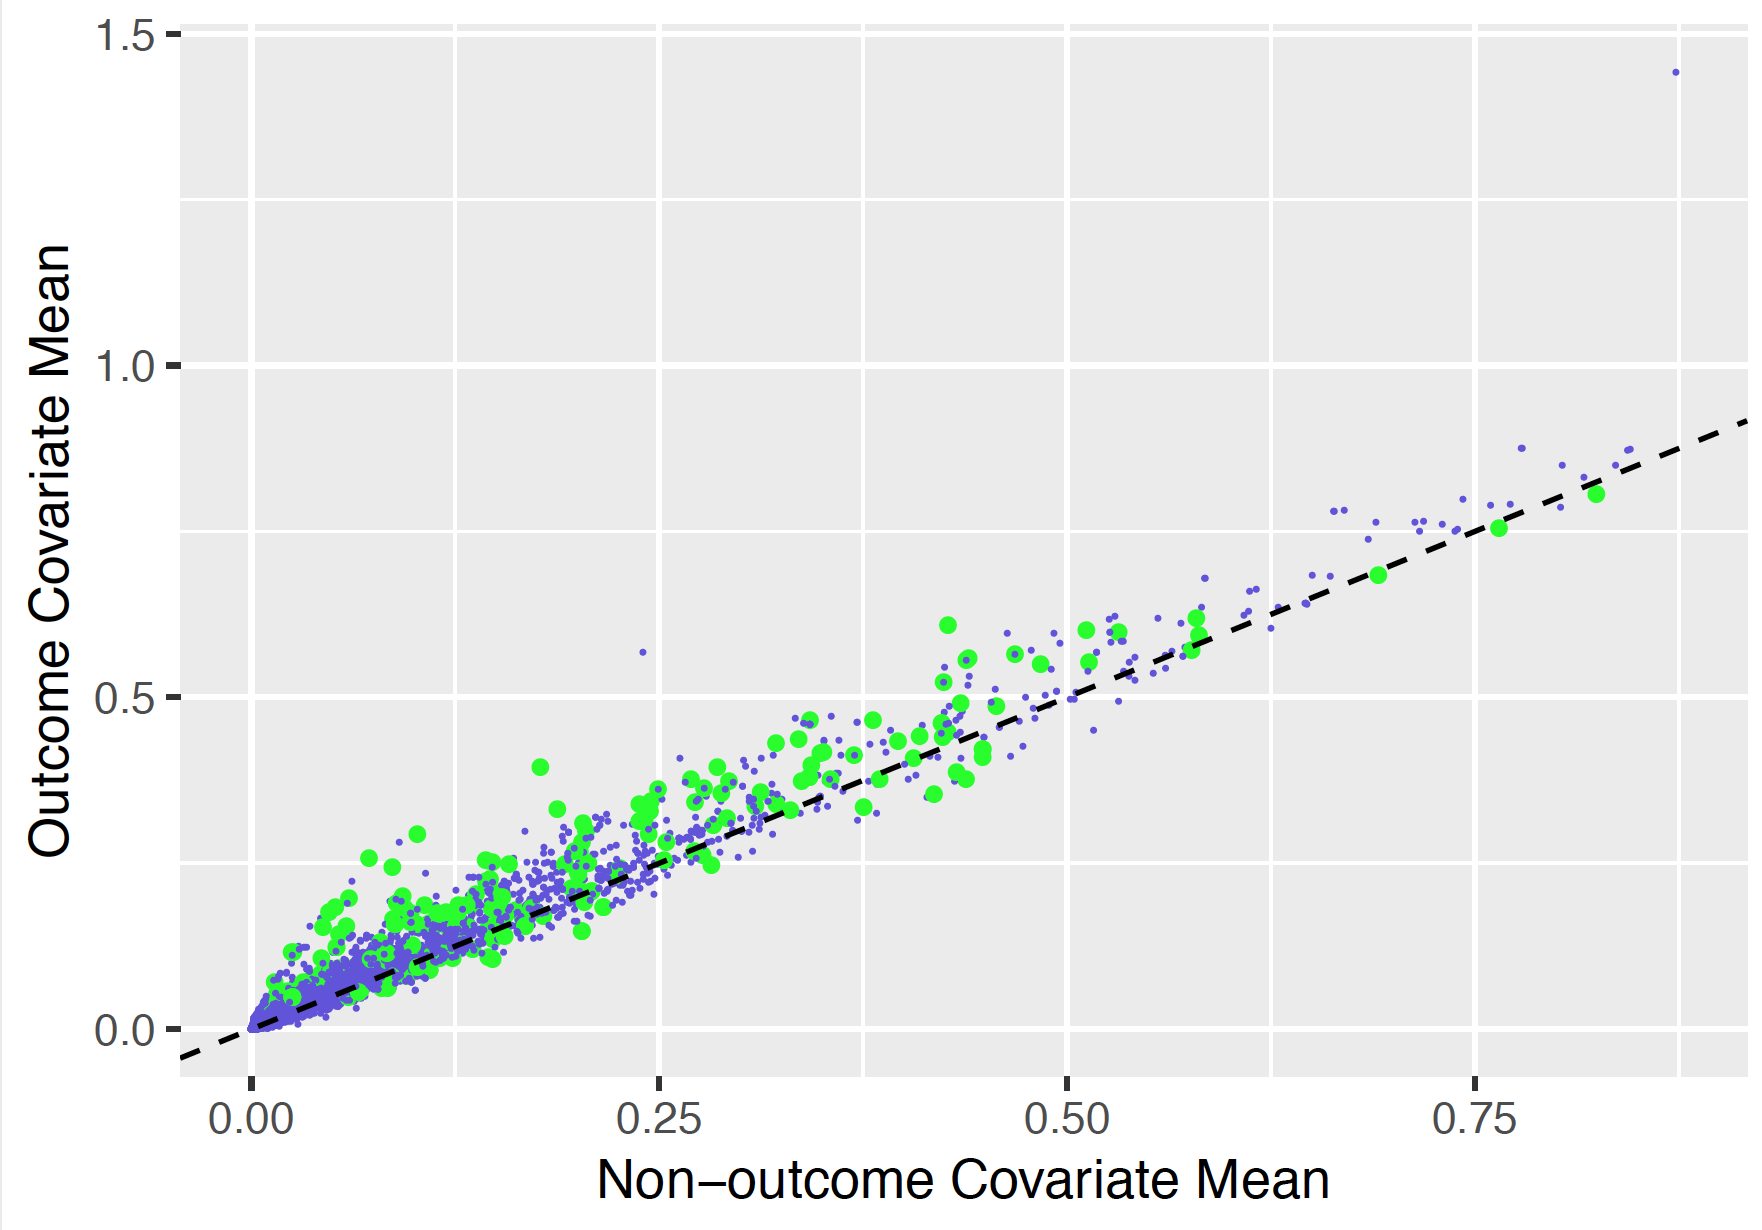
\includegraphics[width=1\linewidth]{images/PatientLevelPrediction/variableScatterplot}

\newpage

\subsection{Precision recall}\label{precision-recall}

Precision (P) is defined as the number of true positives (Tp) over the
number of true positives plus the number of false positives (Fp).

\begin{Shaded}
\begin{Highlighting}[]
\NormalTok{P <-}\StringTok{ }\NormalTok{Tp}\OperatorTok{/}\NormalTok{(Tp}\OperatorTok{+}\NormalTok{Fp)}
\end{Highlighting}
\end{Shaded}

Recall (R) is defined as the number of true positives (Tp) over the
number of true positives plus the number of false negatives (Fn).

\begin{Shaded}
\begin{Highlighting}[]
\NormalTok{R <-}\StringTok{ }\NormalTok{Tp}\OperatorTok{/}\NormalTok{(Tp }\OperatorTok{+}\StringTok{ }\NormalTok{Fn)}
\end{Highlighting}
\end{Shaded}

These quantities are also related to the (F1) score, which is defined as
the harmonic mean of precision and recall.

\begin{Shaded}
\begin{Highlighting}[]
\NormalTok{F1 <-}\StringTok{ }\DecValTok{2}\OperatorTok{*}\NormalTok{P}\OperatorTok{*}\NormalTok{R}\OperatorTok{/}\NormalTok{(P}\OperatorTok{+}\NormalTok{R)}
\end{Highlighting}
\end{Shaded}

Note that the precision can either decrease or increase if the threshold
is lowered. Lowering the threshold of a classifier may increase the
denominator, by increasing the number of results returned. If the
threshold was previously set too high, the new results may all be true
positives, which will increase precision. If the previous threshold was
about right or too low, further lowering the threshold will introduce
false positives, decreasing precision.

For Recall the denominator does not depend on the classifier threshold
(Tp+Fn is a constant). This means that lowering the classifier threshold
may increase recall, by increasing the number of true positive results.
It is also possible that lowering the threshold may leave recall
unchanged, while the precision fluctuates.

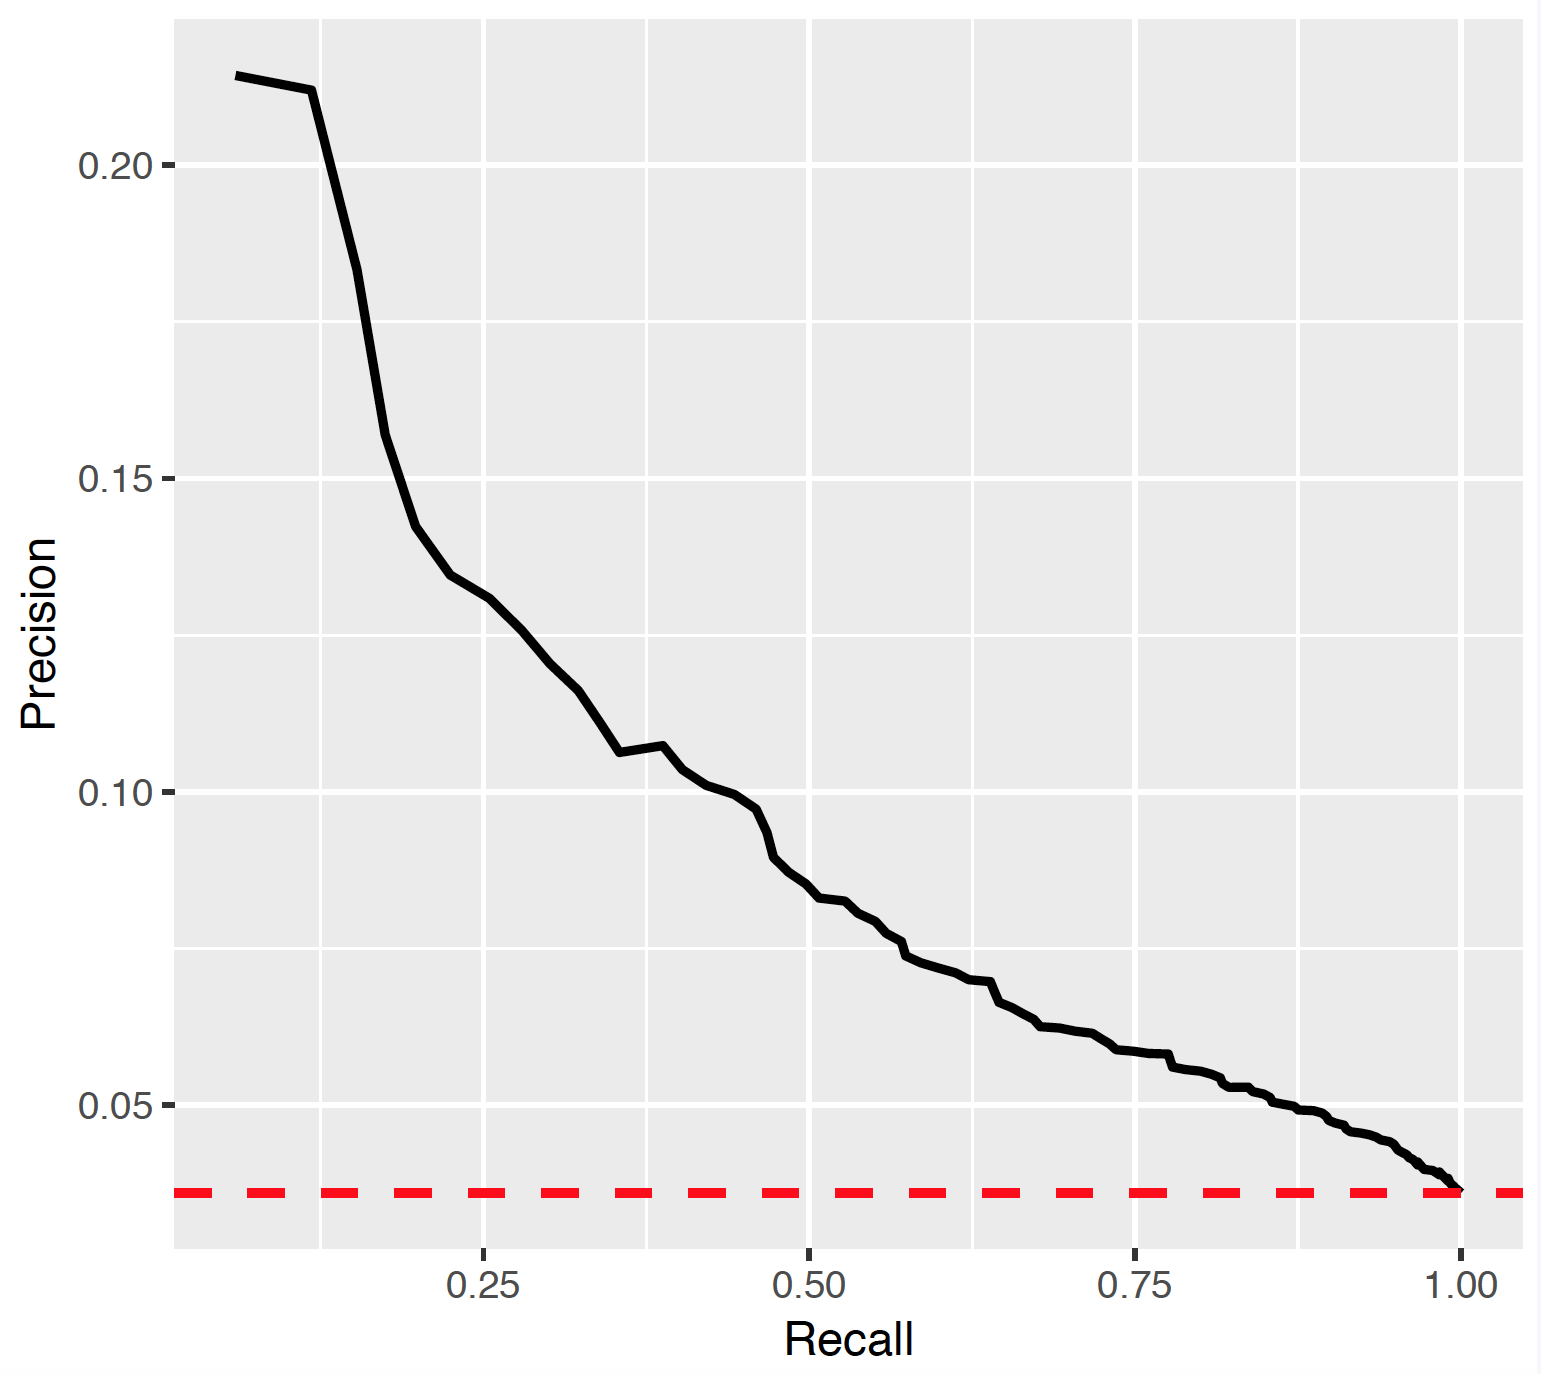
\includegraphics[width=1\linewidth]{images/PatientLevelPrediction/precisionRecall}

\newpage

\subsection{Demographic summary}\label{demographic-summary}

This plot shows for females and males the expected and observed risk in
different age groups together with a confidence area.

The results show that our model is well calibrated across gender and age
groups.

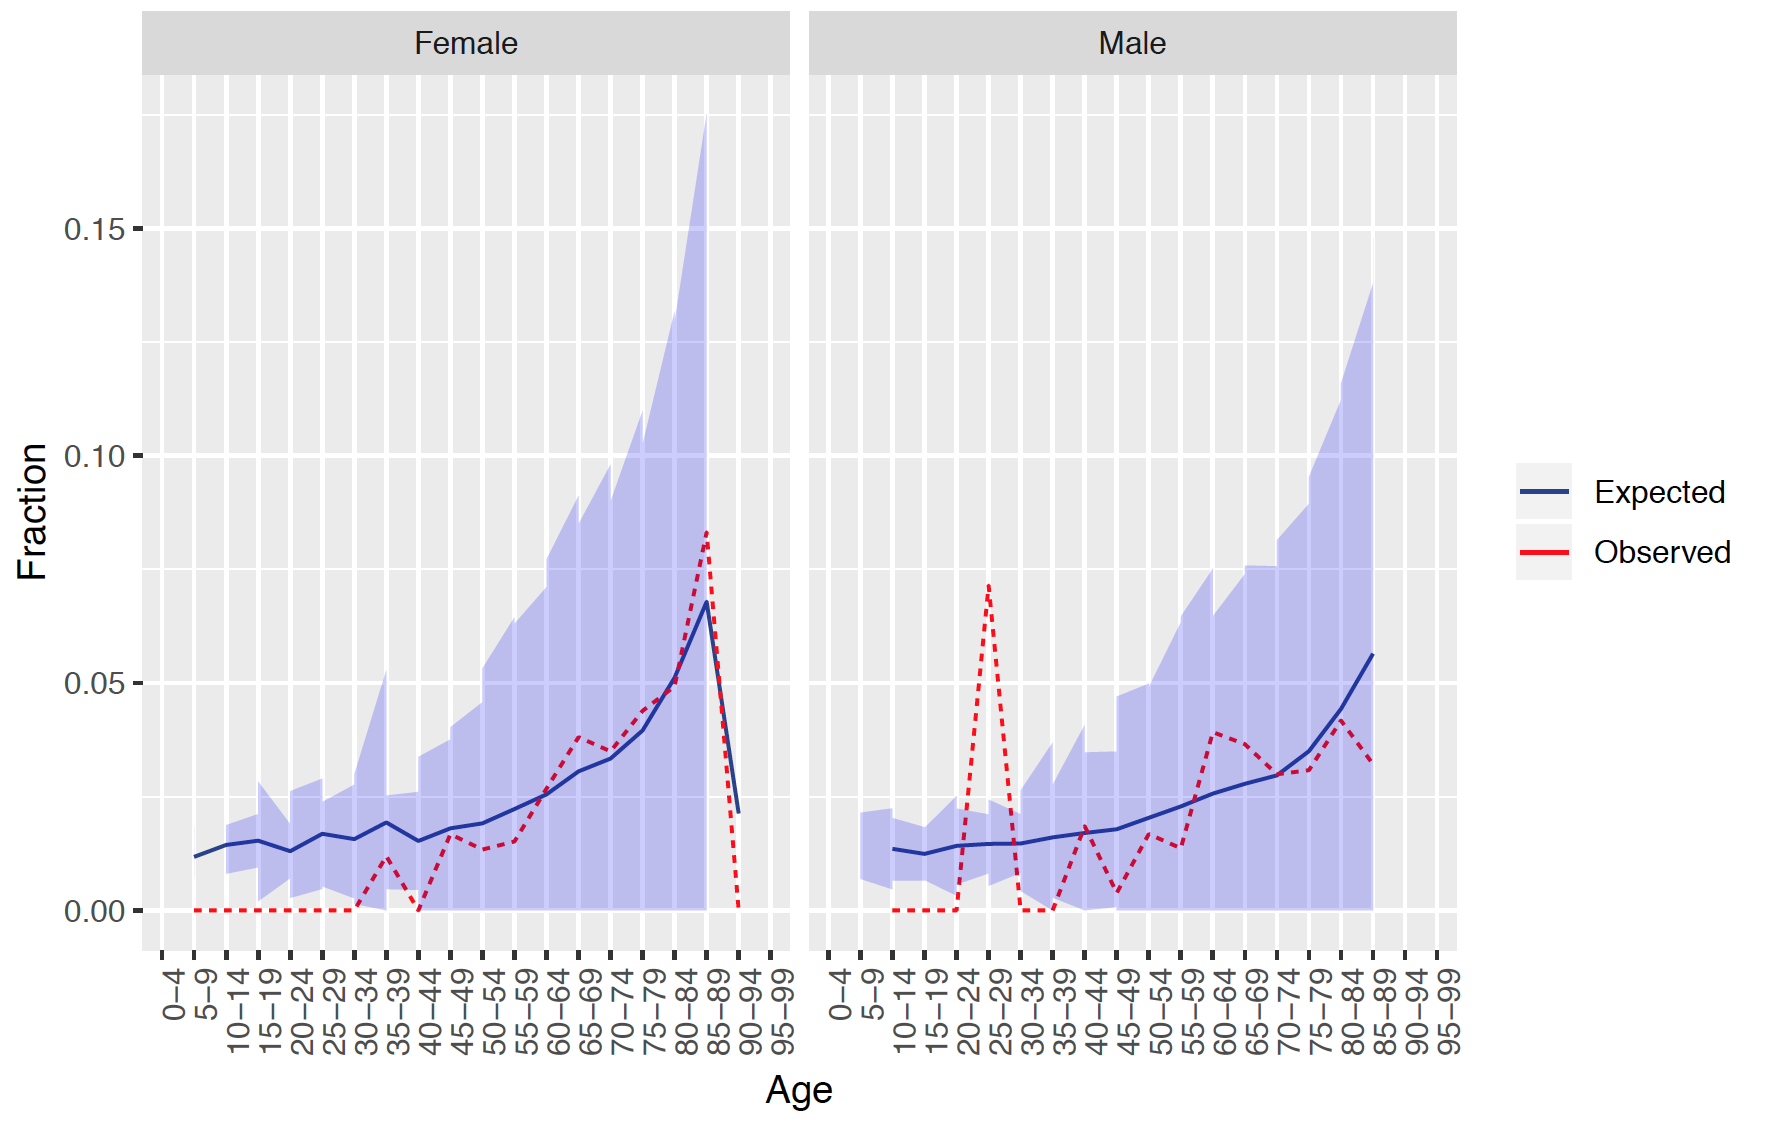
\includegraphics[width=1\linewidth]{images/PatientLevelPrediction/demographicSummary}

\newpage

\section{External validation}\label{external-validation}

We recommend to always perform external validation, i.e.~apply the final
model on as much new datasets as feasible and evaluate its performance.

\begin{Shaded}
\begin{Highlighting}[]
\CommentTok{# load the trained model}
\NormalTok{plpModel <-}\StringTok{ }\KeywordTok{loadPlpModel}\NormalTok{(}\KeywordTok{getwd}\NormalTok{(),}\StringTok{'model'}\NormalTok{)}

\CommentTok{#load the new plpData and create the population}
\NormalTok{plpData <-}\StringTok{ }\KeywordTok{loadPlpData}\NormalTok{(}\KeywordTok{getwd}\NormalTok{(),}\StringTok{'data'}\NormalTok{)}
\NormalTok{population <-}\StringTok{ }\KeywordTok{createStudyPopulation}\NormalTok{(plpData,}
\DataTypeTok{outcomeId =} \DecValTok{2}\NormalTok{,}
\DataTypeTok{includeAllOutcomes =} \OtherTok{TRUE}\NormalTok{,}
\DataTypeTok{firstExposureOnly =} \OtherTok{TRUE}\NormalTok{,}
\DataTypeTok{washoutPeriod =} \DecValTok{365}\NormalTok{,}
\DataTypeTok{removeSubjectsWithPriorOutcome =} \OtherTok{TRUE}\NormalTok{,}
\DataTypeTok{priorOutcomeLookback =} \DecValTok{365}\NormalTok{,}
\DataTypeTok{riskWindowStart =} \DecValTok{1}\NormalTok{,}
\DataTypeTok{requireTimeAtRisk =} \OtherTok{FALSE}\NormalTok{,}
\DataTypeTok{riskWindowEnd =} \DecValTok{365}
\NormalTok{)}

\CommentTok{# apply the trained model on the new data}
\NormalTok{validationResults <-}\StringTok{ }\KeywordTok{applyModel}\NormalTok{(population,plpData,plpModel)}
\end{Highlighting}
\end{Shaded}

To make things easier we also provide a function for performing external
validation of a model across one or multiple datasets:

\begin{Shaded}
\begin{Highlighting}[]
\CommentTok{# load the trained model}
\NormalTok{plpResult <-}\StringTok{ }\KeywordTok{loadPlpResult}\NormalTok{(}\KeywordTok{getwd}\NormalTok{(),}\StringTok{'plpResult'}\NormalTok{)}

\NormalTok{connectionDetails <-}\StringTok{ }\KeywordTok{createConnectionDetails}\NormalTok{(}\DataTypeTok{dbms =} \StringTok{"postgresql"}\NormalTok{,}
                                             \DataTypeTok{server =} \StringTok{"localhost/ohdsi"}\NormalTok{,}
                                             \DataTypeTok{user =} \StringTok{"joe"}\NormalTok{,}
                                             \DataTypeTok{password =} \StringTok{"supersecret"}\NormalTok{)}

\NormalTok{validation <-}\StringTok{ }\KeywordTok{externalValidatePlp}\NormalTok{(}\DataTypeTok{plpResult =}\NormalTok{ plpResult,}
                                  \DataTypeTok{connectionDetails =}\NormalTok{ connectionDetails,}
                                  \DataTypeTok{validationSchemaTarget =} \StringTok{'new_cohort_schema'}\NormalTok{,}
                                  \DataTypeTok{validationSchemaOutcome =} \StringTok{'new_cohort_schema'}\NormalTok{,}
                                  \DataTypeTok{validationSchemaCdm =} \StringTok{'new_cdm_schema'}\NormalTok{,}
                                  \DataTypeTok{validationTableTarget =} \StringTok{'cohort_table'}\NormalTok{,}
                                  \DataTypeTok{validationTableOutcome =} \StringTok{'cohort_table'}\NormalTok{,}
                                  \DataTypeTok{validationIdTarget =} \StringTok{'cohort_id'}\NormalTok{,}
                                  \DataTypeTok{validationIdOutcome =} \StringTok{'outcome_id'}\NormalTok{,}
                                  \DataTypeTok{keepPrediction =}\NormalTok{ T}
\NormalTok{                                  )}
\end{Highlighting}
\end{Shaded}

This will extract the new plpData from the specified schemas and cohort
tables. It will then apply the same population settings and the trained
plp model. Finally, it will evaluate the performance and return the
standard output as \texttt{validation\$performance} and if
keepPrediction is TRUE then it will also return the prediction on the
population as \texttt{validation\$prediction}. They can be inserted into
the shiny app for viewing the model and validation by running:
\texttt{viewPlp(runPlp=plpResult,\ validatePlp=validation\ )}.

If you want to validate on multiple databases available you can insert
the new schemas and cohort tables as a list:

\begin{Shaded}
\begin{Highlighting}[]
\CommentTok{# load the trained model}
\NormalTok{plpResult <-}\StringTok{ }\KeywordTok{loadPlpResult}\NormalTok{(}\KeywordTok{getwd}\NormalTok{(),}\StringTok{'plpResult'}\NormalTok{)}

\NormalTok{connectionDetails <-}\StringTok{ }\KeywordTok{createConnectionDetails}\NormalTok{(}\DataTypeTok{dbms =} \StringTok{"postgresql"}\NormalTok{,}
                                             \DataTypeTok{server =} \StringTok{"localhost/ohdsi"}\NormalTok{,}
                                             \DataTypeTok{user =} \StringTok{"joe"}\NormalTok{,}
                                             \DataTypeTok{password =} \StringTok{"supersecret"}\NormalTok{)}

\NormalTok{validation <-}\StringTok{ }\KeywordTok{externalValidatePlp}\NormalTok{(}\DataTypeTok{plpResult =}\NormalTok{ plpResult,}
                                  \DataTypeTok{connectionDetails =}\NormalTok{ connectionDetails,}
                                  \DataTypeTok{validationSchemaTarget =} \KeywordTok{list}\NormalTok{(}\StringTok{'new_cohort_schema1'}\NormalTok{,}
                                                                \StringTok{'new_cohort_schema2'}\NormalTok{),}
                                  \DataTypeTok{validationSchemaOutcome =} \KeywordTok{list}\NormalTok{(}\StringTok{'new_cohort_schema1'}\NormalTok{,}
                                                                 \StringTok{'new_cohort_schema2'}\NormalTok{),}
                                  \DataTypeTok{validationSchemaCdm =} \KeywordTok{list}\NormalTok{(}\StringTok{'new_cdm_schema1'}\NormalTok{,}
                                                             \StringTok{'new_cdm_schema2'}\NormalTok{),}
                                  \DataTypeTok{validationTableTarget =} \KeywordTok{list}\NormalTok{(}\StringTok{'new_cohort_table1'}\NormalTok{,}
                                                               \StringTok{'new_cohort_table2'}\NormalTok{),}
                                  \DataTypeTok{validationTableOutcome =} \KeywordTok{list}\NormalTok{(}\StringTok{'new_cohort_table1'}\NormalTok{,}
                                                                \StringTok{'new_cohort_table2'}\NormalTok{),}
                                  \DataTypeTok{validationIdTarget =} \StringTok{'cohort_id'}\NormalTok{,}
                                  \DataTypeTok{validationIdOutcome =} \StringTok{'outcome_id'}\NormalTok{,}
                                  \DataTypeTok{keepPrediction =}\NormalTok{ T}
\NormalTok{                                  )}
\end{Highlighting}
\end{Shaded}

\section{Journal paper generation}\label{journal-paper-generation}

We have added functionality to automatically generate a word document
you can use as start of a journal paper. It contains many of the
generated study details and results. If you have performed external
validation these results will can be added as well. Optionally, you can
add a ``Table 1'' that contains data on many covariates for the target
population.

You can create the draft journal paper by running this function:

\begin{Shaded}
\begin{Highlighting}[]
 \KeywordTok{createPlpJournalDocument}\NormalTok{(}\DataTypeTok{plpResult =} \OperatorTok{<}\NormalTok{your plp results}\OperatorTok{>}\NormalTok{,}
                          \DataTypeTok{plpValidation =} \OperatorTok{<}\NormalTok{your validation results}\OperatorTok{>}\NormalTok{,}
                          \DataTypeTok{plpData =} \OperatorTok{<}\NormalTok{your plp data}\OperatorTok{>}\NormalTok{,}
                          \DataTypeTok{targetName =} \StringTok{"<target population>"}\NormalTok{,}
                          \DataTypeTok{outcomeName =} \StringTok{"<outcome>"}\NormalTok{,}
                          \DataTypeTok{table1 =}\NormalTok{ F,}
                          \DataTypeTok{connectionDetails =} \OtherTok{NULL}\NormalTok{,}
                          \DataTypeTok{includeTrain =} \OtherTok{FALSE}\NormalTok{,}
                          \DataTypeTok{includeTest =} \OtherTok{TRUE}\NormalTok{,}
                          \DataTypeTok{includePredictionPicture =} \OtherTok{TRUE}\NormalTok{,}
                          \DataTypeTok{includeAttritionPlot =} \OtherTok{TRUE}\NormalTok{,}
                          \DataTypeTok{outputLocation =} \StringTok{"<your location>"}\NormalTok{)}
\end{Highlighting}
\end{Shaded}

For more details see the help page of the function.

\newpage

\section{Other functionality}\label{other-functionality}

The package has much more functionality than described in this vignette
and contributions have been made my many persons in the OHDSI community.
The table below provides an overview:

\begin{longtable}[]{@{}lll@{}}
\toprule
\begin{minipage}[b]{0.19\columnwidth}\raggedright\strut
Functionality\strut
\end{minipage} & \begin{minipage}[b]{0.54\columnwidth}\raggedright\strut
Description\strut
\end{minipage} & \begin{minipage}[b]{0.19\columnwidth}\raggedright\strut
Vignette\strut
\end{minipage}\tabularnewline
\midrule
\endhead
\begin{minipage}[t]{0.19\columnwidth}\raggedright\strut
Builing Multiple Models\strut
\end{minipage} & \begin{minipage}[t]{0.54\columnwidth}\raggedright\strut
This vignette describes how you can run multiple models
automatically\strut
\end{minipage} & \begin{minipage}[t]{0.19\columnwidth}\raggedright\strut
\href{https://github.com/OHDSI/PatientLevelPrediction/blob/master/inst/doc/BuildingMultiplePredictiveModels.pdf}{\texttt{Vignette}}\strut
\end{minipage}\tabularnewline
\begin{minipage}[t]{0.19\columnwidth}\raggedright\strut
Custom algorithms\strut
\end{minipage} & \begin{minipage}[t]{0.54\columnwidth}\raggedright\strut
This vignette describes how you can add your own custom algorithms in
the framework\strut
\end{minipage} & \begin{minipage}[t]{0.19\columnwidth}\raggedright\strut
\href{https://github.com/OHDSI/PatientLevelPrediction/blob/master/inst/doc/AddingCustomAlgorithms.pdf}{\texttt{Vignette}}\strut
\end{minipage}\tabularnewline
\begin{minipage}[t]{0.19\columnwidth}\raggedright\strut
Ensemble models\strut
\end{minipage} & \begin{minipage}[t]{0.54\columnwidth}\raggedright\strut
This vignette describes how you can use the framework to build ensemble
models, i.e combine multiple models in a super learner\strut
\end{minipage} & \begin{minipage}[t]{0.19\columnwidth}\raggedright\strut
\href{https://github.com/OHDSI/PatientLevelPrediction/blob/master/inst/doc/BuildingEnsembleModels.pdf}{\texttt{Vignette}}\strut
\end{minipage}\tabularnewline
\begin{minipage}[t]{0.19\columnwidth}\raggedright\strut
Deep Learning Models\strut
\end{minipage} & \begin{minipage}[t]{0.54\columnwidth}\raggedright\strut
We have added extensive functionality for Deep Learning including
several architectures in both pyTorch and Keras. These algorithms can be
trained using GPU power\strut
\end{minipage} & \begin{minipage}[t]{0.19\columnwidth}\raggedright\strut
\href{https://github.com/OHDSI/PatientLevelPrediction/blob/master/inst/doc/BuildingDeepLearningModels.pdf}{\texttt{Vignette}}\strut
\end{minipage}\tabularnewline
\begin{minipage}[t]{0.19\columnwidth}\raggedright\strut
Learning curves\strut
\end{minipage} & \begin{minipage}[t]{0.54\columnwidth}\raggedright\strut
Learning curves assess the effect of training set size on model
performance by training a sequence of prediction models on successively
larger subsets of the training set. A learning curve plot can also help
in diagnosing a bias or variance problem as explained below.\strut
\end{minipage} & \begin{minipage}[t]{0.19\columnwidth}\raggedright\strut
\href{https://github.com/OHDSI/PatientLevelPrediction/blob/master/inst/doc/GeneratingLearningCurves.pdf}{\texttt{Vignette}}\strut
\end{minipage}\tabularnewline
\begin{minipage}[t]{0.19\columnwidth}\raggedright\strut
Implementing existing models\strut
\end{minipage} & \begin{minipage}[t]{0.54\columnwidth}\raggedright\strut
This vignette describes how you can implement existing logistic
regression models in the framework, e.g.~as found in literature\strut
\end{minipage} & \begin{minipage}[t]{0.19\columnwidth}\raggedright\strut
\href{https://github.com/OHDSI/PatientLevelPrediction/blob/master/inst/doc/ImplementingExistingModels.pdf}{\texttt{Vignette}}\strut
\end{minipage}\tabularnewline
\bottomrule
\end{longtable}

\section{Demos}\label{demos}

We have added several demos in the package that run on simulated data:

\begin{Shaded}
\begin{Highlighting}[]
\CommentTok{# Show all demos in our package:}
 \KeywordTok{demo}\NormalTok{(}\DataTypeTok{package =} \StringTok{"PatientLevelPrediction"}\NormalTok{)}

\CommentTok{# For example, to run the SingleModelDemo that runs Lasso and shows you how to run the Shiny App use this call}
 \KeywordTok{demo}\NormalTok{(}\StringTok{"SingleModelDemo"}\NormalTok{, }\DataTypeTok{package =} \StringTok{"PatientLevelPrediction"}\NormalTok{)}
\end{Highlighting}
\end{Shaded}

\newpage

\section{Acknowledgments}\label{acknowledgments}

Considerable work has been dedicated to provide the
\href{http://github.com/OHDSI/PatientLevelPrediction}{\texttt{PatientLevelPrediction}}
package.

\begin{Shaded}
\begin{Highlighting}[]
\CommentTok{# citation("PatientLevelPrediction")}
\end{Highlighting}
\end{Shaded}

Further,
\href{http://github.com/OHDSI/PatientLevelPrediction}{\texttt{PatientLevelPrediction}}
makes extensive use of the
\href{http://github.com/OHDSI/Cyclops}{\texttt{Cyclops}} package.

\begin{Shaded}
\begin{Highlighting}[]
\CommentTok{# citation("Cyclops")}
\end{Highlighting}
\end{Shaded}

\textbf{Please reference this paper if you use the PLP Package in your
work:}

\href{http://dx.doi.org/10.1093/jamia/ocy032}{Reps JM, Schuemie MJ,
Suchard MA, Ryan PB, Rijnbeek PR. Design and implementation of a
standardized framework to generate and evaluate patient-level prediction
models using observational healthcare data. J Am Med Inform Assoc.
2018;25(8):969-975.}

This work is supported in part through the National Science Foundation
grant IIS 1251151 and a personalised grant to P.R. Rijnbeek from Janssen
R\&D.

\newpage

\section*{Appendix 1: Study population settings
details}\label{appendix-1-study-population-settings-details}
\addcontentsline{toc}{section}{Appendix 1: Study population settings
details}

In the figures below the effect is shown of the
removeSubjectsWithPriorOutcome, requireTimAtRisk, and includeAllOutcomes
booleans on the final study population. We start with a Target Cohort
with firstExposureOnly = false and we require a washout period = 1095.
We then subset the target cohort based on additional constraints. The
final study population in the Venn diagrams below are colored green.

\begin{enumerate}
\def\labelenumi{\arabic{enumi}.}
\tightlist
\item
  Require minimum time-at-risk for all person in the target cohort.
\end{enumerate}

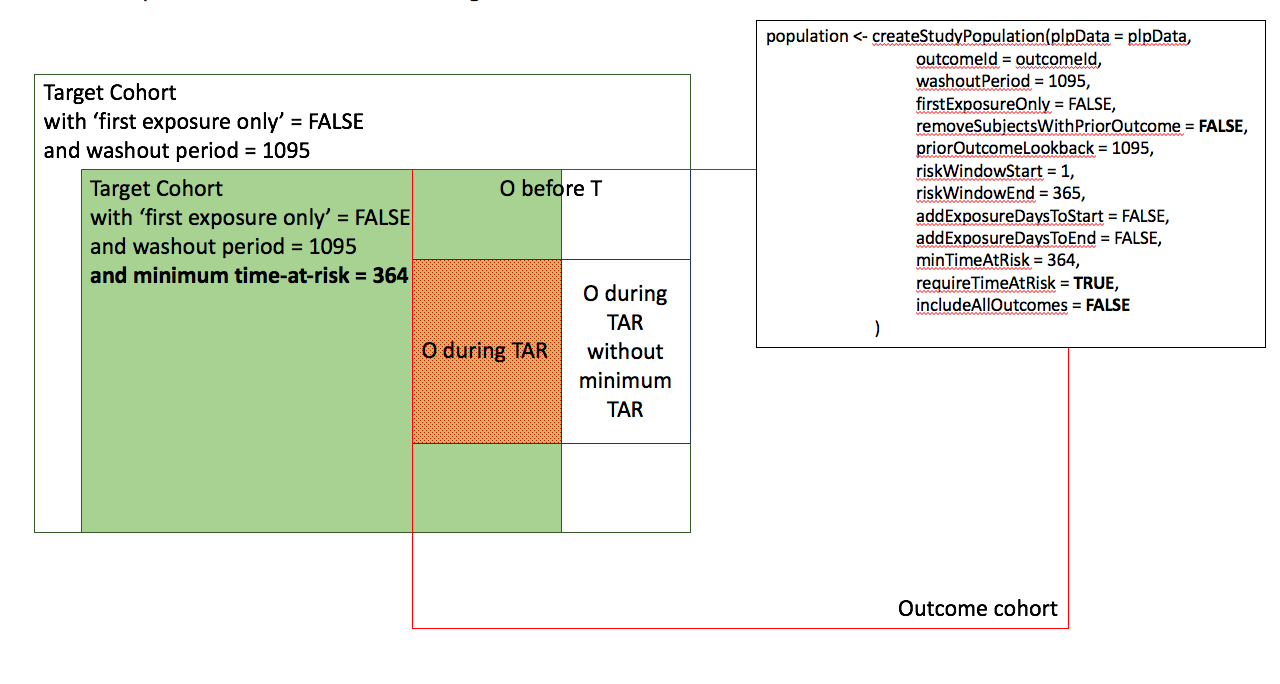
\includegraphics[width=1\linewidth]{images/PatientLevelPrediction/popdef1}

\begin{enumerate}
\def\labelenumi{\arabic{enumi}.}
\setcounter{enumi}{1}
\tightlist
\item
  Require minumum time-at-risk for target cohort, except for persons
  with outcomes during time-at-risk.
\end{enumerate}

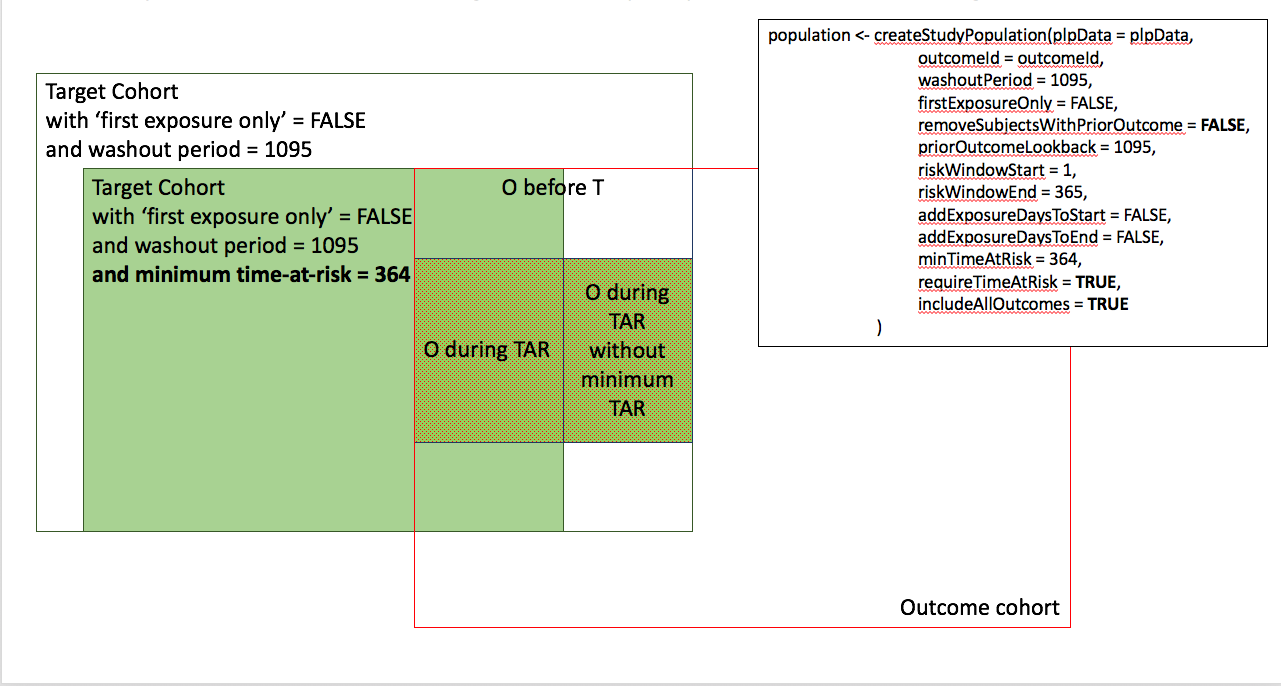
\includegraphics[width=1\linewidth]{images/PatientLevelPrediction/popdef2}

\newpage

\begin{enumerate}
\def\labelenumi{\arabic{enumi}.}
\setcounter{enumi}{2}
\tightlist
\item
  Include all persons in the target cohort exclude persons with prior
  outcomes.
\end{enumerate}

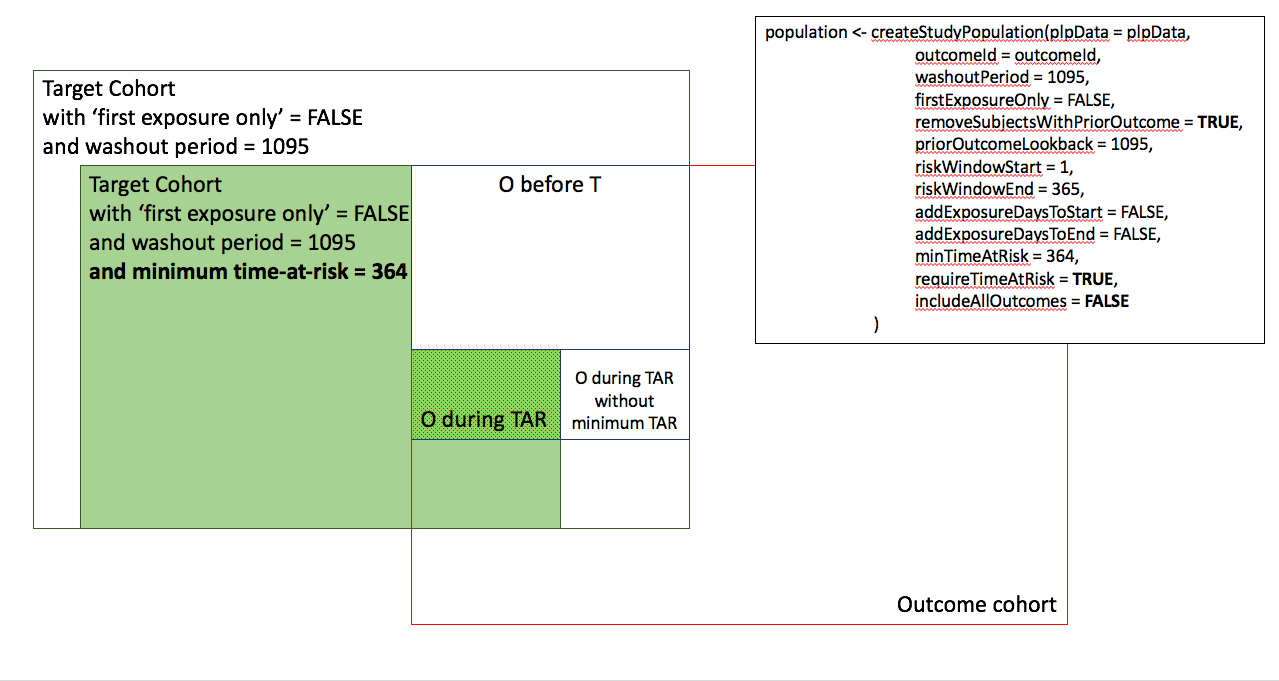
\includegraphics[width=1\linewidth]{images/PatientLevelPrediction/popdef3}

\begin{enumerate}
\def\labelenumi{\arabic{enumi}.}
\setcounter{enumi}{3}
\tightlist
\item
  Require minimum time-at-risk for target cohort, except for persons
  with outcomes during time-at-risk, exclude persons with prior
  outcomes.
\end{enumerate}

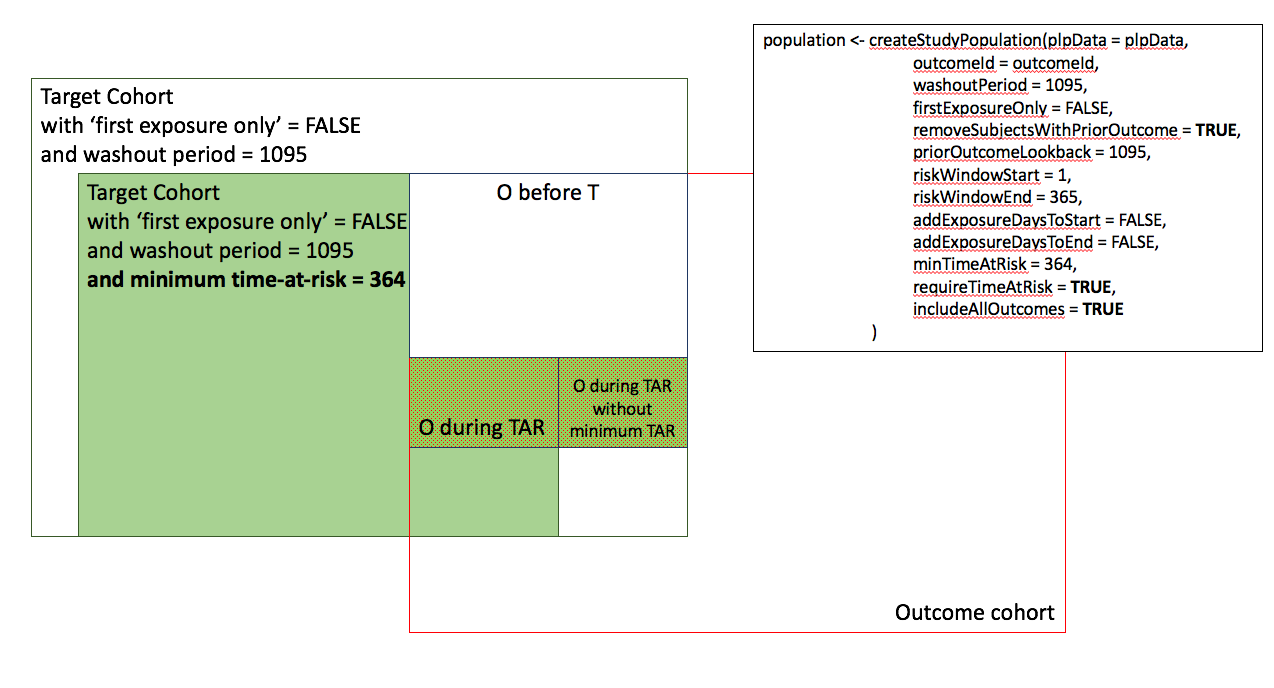
\includegraphics[width=1\linewidth]{images/PatientLevelPrediction/popdef4}

\newpage

\begin{enumerate}
\def\labelenumi{\arabic{enumi}.}
\setcounter{enumi}{4}
\tightlist
\item
  Include all persons in target cohort exclude persons with prior
  outcomes.
\end{enumerate}

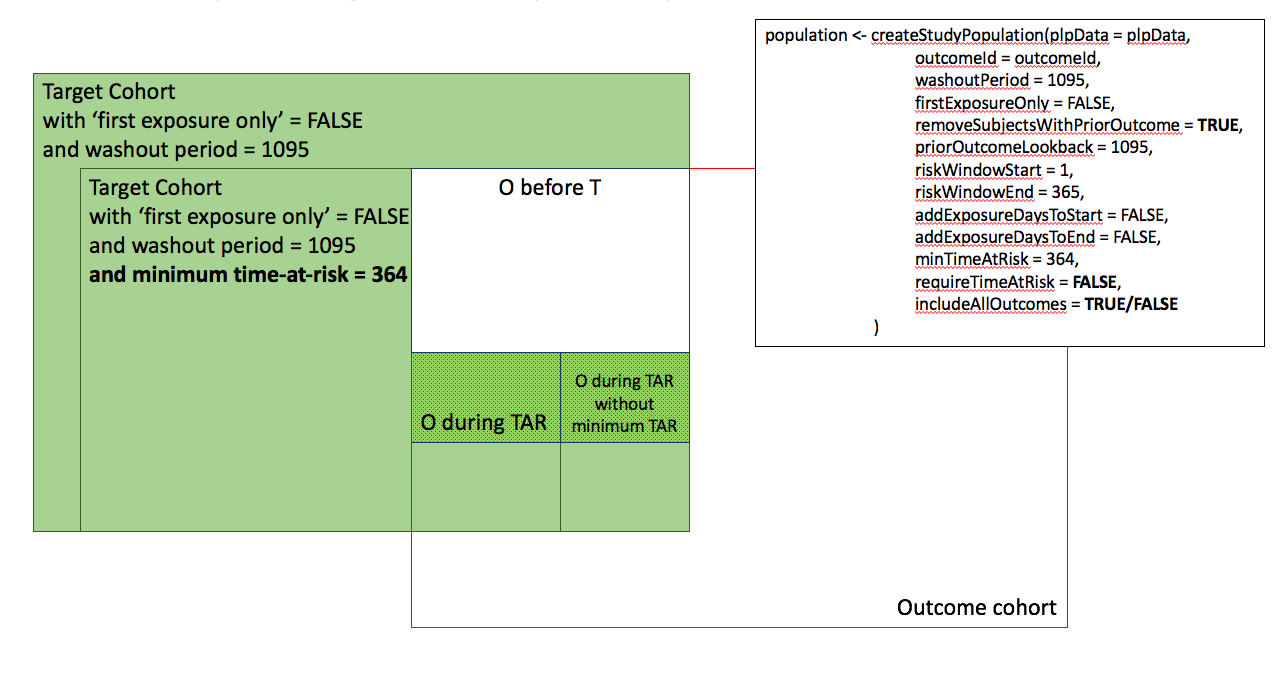
\includegraphics[width=1\linewidth]{images/PatientLevelPrediction/popdef5}

\begin{enumerate}
\def\labelenumi{\arabic{enumi}.}
\setcounter{enumi}{5}
\tightlist
\item
  Include all persons in target cohort.
\end{enumerate}

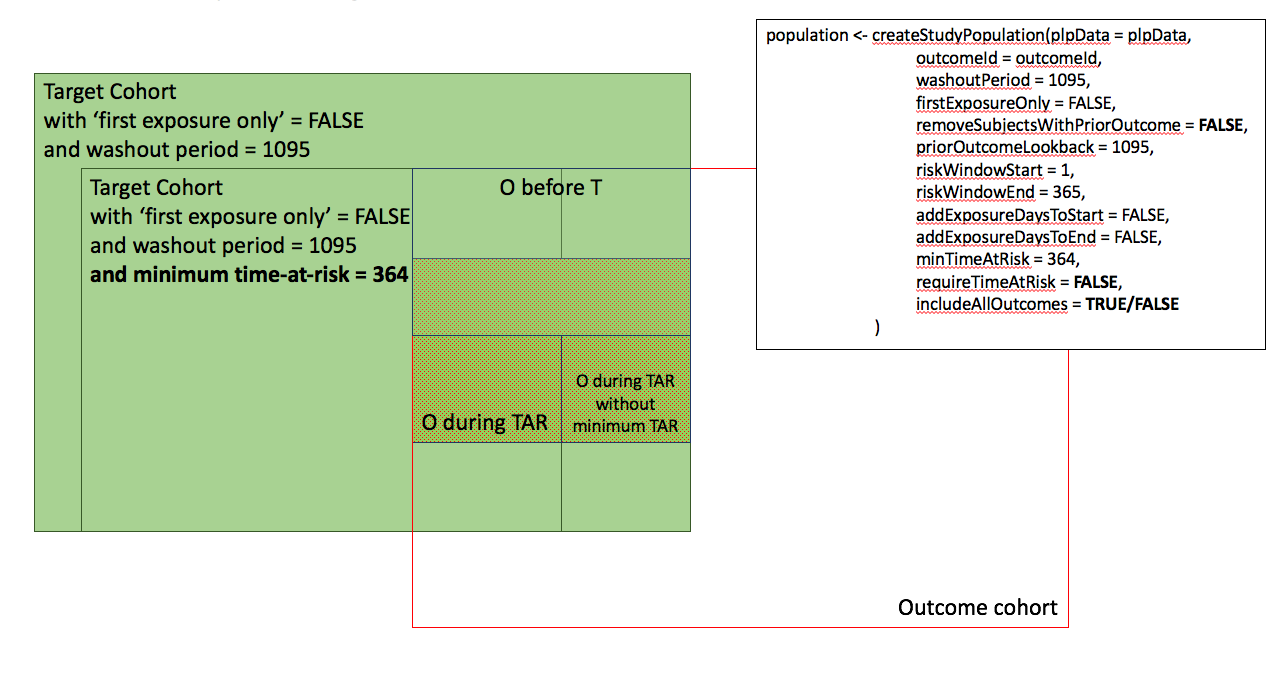
\includegraphics[width=1\linewidth]{images/PatientLevelPrediction/popdef6}

\part{Evidence Quality}\label{part-evidence-quality}

\chapter{Data Quality}\label{DataQuality}

\section{Introduction}\label{introduction}

Kahn et al. define data quality as consisting of three components: (1)
conformance (do data values adhere to do specified standard and
formats?; subtypes: value, relational and computational conformance);
(2) completeness (are data values present?); and (3) plausibility (are
data values believable?; subtypes uniqueness, atemporal; temporal)
\citep{kahn_harmonized_2016}

Kahn additionaly defines two contexts: verification and validation.
Verification focuses on model and data constraints and does not rely on
external reference. Validation focuses on data expectations that are
derived from comparison to a relative gold standard and uses external
knowledge.

\begin{longtable}[]{@{}lll@{}}
\toprule
\begin{minipage}[b]{0.09\columnwidth}\raggedright\strut
Term\strut
\end{minipage} & \begin{minipage}[b]{0.16\columnwidth}\raggedright\strut
Subtype\strut
\end{minipage} & \begin{minipage}[b]{0.67\columnwidth}\raggedright\strut
Validation example\strut
\end{minipage}\tabularnewline
\midrule
\endhead
\begin{minipage}[t]{0.09\columnwidth}\raggedright\strut
Conformance\strut
\end{minipage} & \begin{minipage}[t]{0.16\columnwidth}\raggedright\strut
Value\strut
\end{minipage} & \begin{minipage}[t]{0.67\columnwidth}\raggedright\strut
Providers are only assigned valid medical specialties.\strut
\end{minipage}\tabularnewline
\begin{minipage}[t]{0.09\columnwidth}\raggedright\strut
\strut
\end{minipage} & \begin{minipage}[t]{0.16\columnwidth}\raggedright\strut
Relational\strut
\end{minipage} & \begin{minipage}[t]{0.67\columnwidth}\raggedright\strut
Prescribing provider identifier is present in drug dispensation
data.\strut
\end{minipage}\tabularnewline
\begin{minipage}[t]{0.09\columnwidth}\raggedright\strut
\strut
\end{minipage} & \begin{minipage}[t]{0.16\columnwidth}\raggedright\strut
Computational\strut
\end{minipage} & \begin{minipage}[t]{0.67\columnwidth}\raggedright\strut
Computed eGFR value conforms to the expected value for a test case
patient scenario.\strut
\end{minipage}\tabularnewline
\begin{minipage}[t]{0.09\columnwidth}\raggedright\strut
Completeness\strut
\end{minipage} & \begin{minipage}[t]{0.16\columnwidth}\raggedright\strut
n/a (no subtypes defined)\strut
\end{minipage} & \begin{minipage}[t]{0.67\columnwidth}\raggedright\strut
A drug product withdrawn from the market at a specific absolute historic
date shows expected drop in dispensation.\strut
\end{minipage}\tabularnewline
\begin{minipage}[t]{0.09\columnwidth}\raggedright\strut
Plausibility\strut
\end{minipage} & \begin{minipage}[t]{0.16\columnwidth}\raggedright\strut
Uniqueness\strut
\end{minipage} & \begin{minipage}[t]{0.67\columnwidth}\raggedright\strut
A zip code for a location does not refer to vastly conflicting
geographical areas.\strut
\end{minipage}\tabularnewline
\begin{minipage}[t]{0.09\columnwidth}\raggedright\strut
\strut
\end{minipage} & \begin{minipage}[t]{0.16\columnwidth}\raggedright\strut
Atemporal\strut
\end{minipage} & \begin{minipage}[t]{0.67\columnwidth}\raggedright\strut
Use of a medication (by age group) for a specific disease agrees with
the age pattern for that disease.\strut
\end{minipage}\tabularnewline
\begin{minipage}[t]{0.09\columnwidth}\raggedright\strut
\strut
\end{minipage} & \begin{minipage}[t]{0.16\columnwidth}\raggedright\strut
Temporal\strut
\end{minipage} & \begin{minipage}[t]{0.67\columnwidth}\raggedright\strut
Temporal pattern of an outbreak of a disease (e.g., Zika) agrees with
external source pattern.\strut
\end{minipage}\tabularnewline
\bottomrule
\end{longtable}

Kahn introduces the term \emph{data quality check} (sometimes refered to
as data quality rule) that tests whether data conform to a given
requirement (e.g., implausible age of 141 of a patient (due to incorrect
birth year or missing death event)). In support of checks, he also
defines \emph{data quality measure} (sometimes refered to as
pre-computed analysis) as data analysis that supports evaluation of a
check. For example, distribution of days of supply by drug concept.

Two types of DQ checks can be distinguished\citep{weiskopf_methods_2013}

\begin{itemize}
\tightlist
\item
  general checks
\item
  study-specific checks
\end{itemize}

From the point of researcher analyzing the data, the desired situation
is that data is free from erros that could have been prevented.
\emph{ETL data errors} are errors introduced during
extract-tranform-load proces. A special type of ETL data error is
\emph{mapping error} that results from incorrect mapping of the data
from the source terminology (e.g., Korean national drug terminology)
into the target data model's standard terminology (e.g., RxNorm and
RxNorm Extension). A \emph{source data error} is an error that is
already present in the source data due to various cuases (e.g., human
typo during data entry).

Data quality can also be seen as a component in a larger effort refered
to as \emph{evidence quality} or \emph{evidence validation}. Data
quality would fall in this framework under \emph{data validation}.

\section{Achilles Heel tool}\label{achilles-heel-tool}

Since 2014, a component of the OHDSI Achilles tool called Heel was used
to check data quality.\citep{huser_methods_2018}

\subsection{Precomputed Analyses}\label{precomputed-analyses}

In support of data characterization, Achilles tool pre-computes number
of data analyses. Each pre-computed analysis has an analysis ID and a
short description of the analysis. For example, ``715: Distribution of
days\_supply by drug\_concept\_id'' or ``506: Distribution of age at
death by gender''. List of all pre-computed analyses (for Achilles
version 1.6.3) as available at
\url{https://github.com/OHDSI/Achilles/blob/v1.6.3/inst/csv/achilles/achilles_analysis_details.csv}

Achilles has more than 170 pre-computed analysis that support not only
data quality checks but also general data characterization (outside data
quality context) such as data density visualizations. The
pre-computations are largely guided by the CDM relational database
schema and analyze most terminology-based data columns, such as
condition\_concept\_id or place\_of\_service\_concept\_id.
Pre-computations results are stored in table ACHILLES\_RESULTS and
ACHILLES\_RESULTS\_DIST.

\subsection{Example DQ check}\label{example-dq-check}

In complete data about general population, a range of services is
provided by a range of providers (with many specialties). A data
completness rule with rule\_id of 38 evaluates data completness in the
PROVIDER table. Checking optional fields in CDM (such as provider
specialty) lead to a notification severity output. Analysis Rule 38
triggers a notification if count of distinct specialties \textless{}2.
It relies on a derived measure \texttt{Provider:SpeciatlyCnt}. The rule
SQL-formulated logic can be found here:
\url{https://github.com/OHDSI/Achilles/blob/v1.6.3/inst/sql/sql_server/heels/serial/rule_38.sql}

\subsection{Overview of existing DQ Heel
checks}\label{overview-of-existing-dq-heel-checks}

Achilles developers maintain a list of all DQ checks in an overview
file. For version 1.6.3, this overview is available here
\url{https://github.com/OHDSI/Achilles/blob/v1.6.3/inst/csv/heel/heel_rules_all.csv}
Each DQ check has a rule\_id.

Checks are classified into CDM conformance checks and DQ checks.

Depending on the severity of the problem, the Heel output can be error,
warning or notification.

\section{Study-specific checks}\label{study-specific-checks}

The chapter has so far focused on general DQ checks. Such checks are
executed regardless of the single research question context. The
assumption is that a researcher would formulate additional DQ checks
that are required for a specific research question.

We use case studies to demostrate study-specific checks.

\subsection{Outcomes}\label{outcomes}

For an international analysis, part of OHDSI study diagnostics (for a
give dataset) may involve checking whether coding practices (that are
country specific) affect a cohort definition. A stringent cohort
definition may lead to zero cohort size in one (or multiple dataesets).

\subsection{Laboratory data}\label{laboratory-data}

A diabetes study may utilize HbA1c measurement. A 2018 OHDSI study
(\url{https://www.ncbi.nlm.nih.gov/pubmed/30646124}) defined a cohort
`HbA1c8Moderate' (see
\url{https://github.com/rohit43/DiabetesTxPath/blob/master/inst/settings/CohortsToCreate.csv})

\chapter{Software Validity}\label{SoftwareValidity}

\chapter{Clinical Validity}\label{ClinicalValidity}

\chapter{Method Validity}\label{MethodValidity}

\part{OHDSI Studies}\label{part-ohdsi-studies}

\chapter{Study steps}\label{StudySteps}

Writing the protocol, OHDSI style:
\url{http://www.ohdsi.org/web/wiki/lib/exe/fetch.php?media=projects:workgroups:wg_study_protocols_eastern_hemisphere.pptx}

Study reproducibility (Martijn has some slides that might help:
\url{http://www.ohdsi.org/web/wiki/lib/exe/fetch.php?media=projects:workgroups:wg_study_reproducability.pptx}
)

\chapter{OHDSI Network Research}\label{NetworkResearch}

Contributors: Greg Klebanov, Vojtech Huser, list others

What is OHDSI Network?

\begin{itemize}
\tightlist
\item
  OHDSI Community and Network Research
\item
  International Open Science Networks
\item
  OHDSI US
\item
  OHDSI EU and EHDEN
\item
  OHDSI APAC
\end{itemize}

OHDSI Network Study Process

\begin{itemize}
\tightlist
\item
  Goals
\item
  Workflow Overview
\item
  Structure of Studies
\item
  Protocol and IRB issues
\item
  Existing framework (de-identified {[}time shifted{]} OMOP dataset
  under existing IRB protocol
\item
  Overcoming Network Study Challenges
\item
  Data Privacy, Security and Compliance
\item
  Data Quality
\item
  Running OHDSI Methods in Isolated Environment
\item
  OMOP CDM Versioning
\end{itemize}

Tools, Platforms and Study Automation * OHDSI Methods support for
Network Studies * LEGEND (should we have it here?) * OHDSI ARACHNE
Network Platform

Opportunities, future trends and Roadmap

\section{OHDSI Network Study
Examples}\label{ohdsi-network-study-examples}

\subsection{Endometriosis study}\label{endometriosis-study}

An endometriosis characterization study (available at
\url{https://github.com/molliemckillop/Endometriosis-Phenotype-Characterization})
works with two cohorts. They are defined in cohorts.csv file (see here
\url{https://github.com/molliemckillop/Endometriosis-Phenotype-Characterization/blob/master/inst/settings/cohorts.csv}).

After creating a cohort table, it is populated by executing this command
here by infering a name of a `.sql' file from the previously defined
cohort file. A createCohorts function is executed next. (see
\url{https://github.com/molliemckillop/Endometriosis-Phenotype-Characterization/blob/master/R/createCohorts.R}).
An SQL file that is generated by Atlas populates the cohort table with
specific person\_ids that fulfill the cohort definition.

\section{Excercises}\label{excercises}

\subsection{Defining a cohort}\label{defining-a-cohort}

Q: Study the code for the x study and determine whether the cohort
definition is available on the public OHDSI server. It if it, what is
the cohort ID there?

A:

\appendix


\chapter{Glossary}\label{Glossary}

Cohort A cohort is a list of person\_ids with start and end date. It is
stored in a study specific cohort table or a CDM specified cohort table
can also be used. Cohort can be represented as .json file. It is used
for import and export but not during an analysis. OHDSI tools use SQL so
Atlas also generates a .sql file that creates the cohort during
analysis.

Parametized SQL code An SQL code that allows for use of parameters.
Parameters are prefixed with @. Such code has to be ``rendered''.
Synonym: OHDSI SQL code.

\bibliography{book.bib,packages.bib}


\end{document}
